\documentclass[a4paper, 12pt, abstract=on, bibliography=totoc]{scrreprt}

\newcommand*{\Title}{{A Novel Liquid Argon Time Projection Chamber Detector: The ArgonCube Concept}}
\newcommand*{\Author}{{Damian Goeldi}}
\newcommand*{\Supervisor}{{Prof.\ Dr.\ A.\ Ereditato}}
\newcommand*{\Dean}{{Prof.\ Dr.\ (Initiale Name)}}
\newcommand*{\Date}{{(Pr\"ufungsdatum)}}

\usepackage{scrhack} % fix warnings due to packages using deprecated KOMA-Script commands

\usepackage[british]{babel} % set babel to british rather than american
\usepackage[utf8]{inputenc} % utf8 support in source code
\usepackage{lmodern} % better support for special characters in pdf
\usepackage[T1]{fontenc}
\usepackage{textcomp}

\usepackage[autostyle]{csquotes} % recommended by biblatex
\usepackage{xpatch} % recommended by biblatex
\usepackage[backend=biber, firstinits, sorting=none, backref=true]{biblatex} % much more flexible than BibTeX

\usepackage{ifdraft}
\usepackage{setspace} % make corrections easier
\usepackage[pagewise]{lineno}
\usepackage[colorinlistoftodos, obeyFinal]{todonotes}

\usepackage{fancyvrb} % advanced verbatim
\usepackage{mathtools} % math packages
\usepackage{amsfonts}
\usepackage{amssymb}
\usepackage{physics}
\usepackage[version=4]{mhchem}
\usepackage[retainorgcmds]{IEEEtrantools} % advanced equation arrays
\usepackage{siunitx} % write units properly
\usepackage{tabu} % much better than tabular
\usepackage{listings} % list source code
\usepackage{chngcntr} % continuous footnote numeration (in chapter)
\usepackage{pdfpages} % insert PDF pages
\usepackage{xcolor, graphicx} % for graphics, breaks (e)ps support
\usepackage{pdflscape} % landscape pages

\addbibresource{thesis.bib} % .bib file for biblatex (.bib is required)

\pagestyle{headings} % instead of fancyhdr which is not recommended with KOMA script classes

\VerbatimFootnotes % needed for verbatim in footnotes (obviously :)

\hyphenpenalty=1000 % de/increase some formatting penalties to get nicer result
\tolerance=5000 % tolerance for total badness without line break
\setlength{\parskip}{0pt plus 3pt} % add some "rubber" space between paragraphs to omit widows and orphans

\sisetup{separate-uncertainty=true}

% make corrections easier
\newcommand{\cjames}[2][]{\todo[author={James Sinclair}, color=green, #1]{#2}}
\ifoptionfinal{}{
	\doublespacing
	\linenumbers
}

\newcommand*{\m}{\mathrm}
\newcommand*{\qraq}{\quad \rightarrow \quad}
\newcommand*{\Chapter}{chapter} % used in starred chapters to store the chapter name to access it conveniently with all the commands needed there

\newcommand*{\AT}{{ARGONTUBE}}
\newcommand*{\AC}{{ArgonCube}}
\newcommand*{\dune}{{DUNE}}
\newcommand*{\uboone}{{MicroBooNE}}
\newcommand*{\sbnd}{SBND}
\newcommand*{\icarus}{{ICARUS}}

\newcommand*{\lar}{{LAr}}
\newcommand*{\lartpc}{LArTPC}

\usepackage[pdftex, unicode, bookmarks, pdffitwindow, pdftitle={\Title}, pdfauthor={\Author}, colorlinks=false]{hyperref} % should be last command in preamble

\begin{document}

\graphicspath{{graphics/}}

\pagenumbering{roman}

\begin{titlepage}
	\begin{center}
		\null
		\vfill
		\textbf{\LARGE\Title}\\[20mm]
		\textbf{\large Inauguraldissertation}\\
		{\large der Philosophisch-naturwissenschaftlichen Fakultät}\\
		{\large der Universität Bern}\\[20mm]
		{\large vorgelegt von}\\[10mm]
		\textbf{\Large\Author}\\[10mm]
		{\large von Sennwald SG}\\[20mm]
		{\large Leiter der Arbeit}\\
		\textbf{\large\Supervisor}\\[10mm]
		{\large Albert Einstein Center for Fundamental Physics}\\
		{\large Laboratory for High Energy Physics}\\
		{\large Physics Institute}\\
		\vfill
	\end{center}
\end{titlepage}
\cleardoublepage
\begin{titlepage}
	\begin{center}
		\null
		\vfill
		\textbf{\LARGE\Title}\\[20mm]
		\textbf{\large Inauguraldissertation}\\
		{\large der Philosophisch-naturwissenschaftlichen Fakultät}\\
		{\large der Universität Bern}\\[20mm]
		{\large vorgelegt von}\\[10mm]
		\textbf{\Large\Author}\\[10mm]
		{\large von Sennwald SG}\\[20mm]
		{\large Leiter der Arbeit}\\
		\textbf{\large\Supervisor}\\[10mm]
		{\large Albert Einstein Center for Fundamental Physics}\\
		{\large Laboratory for High Energy Physics}\\
		{\large Physics Institute}\\[10mm]
		{\large Von der Philosophisch-naturwissenschaftlichen Fakultät angenommen.}\\[10mm]
		\begin{tabu} to \textwidth {p{8cm}l}
			{\large Bern, \Date} &	{\large Der Dekan:} \\
			&						{\large\Dean}
		\end{tabu}
		\vfill
	\end{center}
\end{titlepage}
\cleardoublepage
\thispagestyle{empty}
To Bäschu.

\bigskip

It was always inspiring and great fun conducting research with you.
\cleardoublepage
\begin{abstract}

There is this big problem which people are trying to solve with inferior technology. Silly people. They should use the technology proposed here, it is much better.  

\end{abstract}
\cleardoublepage
\renewcommand{\Chapter}{{Preface}}
\chapter*{\Chapter}
\chaptermark{\Chapter}

\todo[inline, color=red]{preface}
Chapter~\ref{chap:nu-detection} will give an overview of the history of neutrino detectors, describe the current state of the field and then introduce the most relevant physics.
Giunti and Kim provide a more detailed history of neutrino physics.~\cite{giunti}

The work in Chapter~\ref{chap:dune-nd} was a collaboration with the neutrino group at Lawrence Berkeley National Laboratory (LBNL).
In particular, they provided the simulation tool, Argon Box, as well as the raw simulation data.
The \Pgpz pile-up study was done by the author with advice from C.\ Marshall from LBNL.

\listoftodos
\tableofcontents
\listoffigures
\listoftables
\lstlistoflistings

\cleardoublepage % without this, previous page is already arabic; pay attention to twoside layout!
\pagenumbering{arabic}

\todo[inline, caption={Check preamble}]{Check preamble.
In particular, putting hyperref to the end of the preample as suggested by ``The not so short introduction to \LaTeX{}'' produces warnings about duplicate footnote references.
Could it also be caused by TODOs?}
\todo[inline]{Replace backslash space after commands by braces}
\todo[inline]{Optimise float placement, short captions for lists of floats}
\todo[inline]{Dean, Date}
\cjames{test}
\cjames[inline]{inline test}

\chapter{Introduction}
\label{chap:introduction}

\todo[inline, color=red]{introduction}
To measure the remaining unknown parameters of the PMNS matrix and the mass hierarchy in neutrino oscillation physics, detectors with masses of orders of magnitude larger than so far are needed.
There are two obvious demonstrated choices.
Water Cherenkov detectors provide a large cost-efficient target mass which makes them interesting for proton decay searches as well.
A \lartpc{} on the other hand is an imaging detector providing precise tracking, while simultaneously acting as a homogeneous calorimeter with a precise measurement of energy deposited.
Furthermore, the 3D resolution of these detectors allows for an efficient $e$ $\gamma$ separation, thus reducing the $\pi^0$ background in $\nu_e$ identification.

For a TPC to work, the detection medium needs to have a low electronegativity.
Noble gases are an obvious choice for this.
To provide a high target mass, they are liquified.
The ideal choice would be LXe which therefore is used for low volume experiments such as neutrino-less double beta decay and dark matter searches.
The drawback of xenon is that it is expensive and rare.
Besides, \lar{} has a longer radiation length than LXe and produces a comparable number of photons per \si{\mega\electronvolt}, it is also abundant and relatively cheap.

Future neutrino oscillation physics experiments aim to measure the $\delta_{\m{CP}}$ phase and determine the neutrino mass hierarchy.
With the recent measurement of the $\theta_{13}$ mixing angle, new experiments can be tuned to the right parameter space to be most sensitive in the most probable regions.
Both measurements require much higher statistics than contemporary experiments have achieved.
In turn, higher statistics require that the neutrino flux is increased, and an increase in detection efficiencies.
Efficiency is improved by increasing the size of the detector by up to two orders of magnitude in comparison to the current generation, the increase in size also improves event containment.

These imposed requirements lead to several new challenges for the detector design.
Higher flux beams put higher demands on the precision of the trigger system to reach reasonable trigger efficiencies and purities.
Additionally, \lartpc{}s have some intrinsic issues in high-flux particle beams, most of these issues stem from the detector volume required for the containment of events:
The long drift-times lead to event pile-up and also require higher voltages and higher purity argon, and unconfined scintillation light makes it harder to use a light detection system as a coincidence trigger.
Event pile-up is worsened still by the intrinsic reconstruction ambiguities of the conventional wire readout.
The complexity of event reconstruction due to the projective nature of wires further reduces the ability of the trigger system.
As well as being notoriously fragile, wire readouts and their associated framework are a major limiting factor in detector design.
The most inhibitive drawback to monolithic detectors is the down-time cost involved in repair or upgrade work.
Independent of future neutrino experiments, the solution of all those problems will lead to next generation \lartpc{}s bringing huge improvements for all future applications of such detectors.
\chapter{Neutrino Detection}
\label{chap:nu-detection}

Neutrino physics has seen massive progress from first detection \num{60}~years ago to planned billion dollar experiments in the near future.
This chapter will give an overview of the history of neutrino detectors, describe the current state of the field and then introduce the most relevant physics.

\section{History}
In 1914, Chadwick proved that the energy spectrum of the $\beta$-decay was continuous.~\cite{contBeta}
As an explanation for this, Wolfgang Pauli in 1930 proposed a new neutral, weakly interacting fermion to the \emph{Radioactive Ladies and Gentlemen}~\cite{pauliLetter} which he called the \emph{neutron}.
However, the same Chadwick in 1932 discovered the particle we today call neutron.~\cite{neutron}
Upon this, Fermi proposed the name \emph{neutrino} and a little later came up with a new theory for $\beta$-decay.~\cite{betaDecay}

It took almost another quarter of a century until the neutrino was experimentally detected for the first time by Reines and Cowan in 1956.~\cite{reinesCowan}
They built a detector for the reaction
\begin{IEEEeqnarray}{rCl}
	\label{eq:nu-detection_reinesCowan}
	\nueb + p & \rightarrow & e^+ + n
\end{IEEEeqnarray}
and put it next to the nuclear reactor of the Savannah River Plant in South Carolina, US.
It consisted of two water tanks sandwiched in between three liquid scintillator tanks with photomultiplier tubes (PMTs) on the sidewalls.
The water was the target to induce the above reaction while the scintillator tanks had the task of detecting the resulting positron and neutron.
A free positron slows down in matter and eventually gets captured by a shell electron which produces two back-to-back $\gamma$s with an energy of \SI{511}{\kilo\electronvolt} each.
These produce scintillation light in the two adjacent tanks and thus can be detected by forming a coincidence of the PMTs of the two tanks.
Neutron detection is achieved by doping the water target with cadmium which captures the free neutrons producing multiple $\gamma$s that can again be detected using the coincidence of the two adjacent scintillator tanks.
The neutron capture is much slower than the positron one.
Therefore, the process from Equation~\eqref{eq:nu-detection_reinesCowan} produces a very distinct signal in the detector consisting of a pulse with a lower amplitude from the positron capture and another one with a higher amplitude from the neutron capture a few \si{\micro\second} later.
Backgrounds can be efficiently rejected employing this technique.
That drawback is that detection is limited to the \nueb{} interaction in Equation~\eqref{eq:nu-detection_reinesCowan}.

In 1962, Lederman et al.\ proved the existence of the \numu{} at the Alternating Gradient Synchrotron (AGS) at Brookhaven National Laboratory (BNL) in New York, US.~\cite{numu}
For the first time, they produced \numu{}s using an accelerator.
The protons from the AGS were guided onto a beryllium target producing pions which in turn decay according to
\begin{IEEEeqnarray}{rCl}
	\label{eq:nu-detection_pion-decay}
	\pi^+ & \rightarrow & \mu^+ + \numub \qand \\
	\pi^- & \rightarrow & \mu^- + \numu
\end{IEEEeqnarray}
producing a beam of muon (anti)neutrinos.
\emph{Spark chambers} were used to detect the neutrinos.
They were placed behind a \SI{13.5}{\metre} wall of iron shielding used to stop the muons and remaining hadrons from the beam.

A spark chamber consists of several parallel conducting plates immersed in a counting gas, typically a mixture of helium and neon.
Every other plate is connected to a pulsed high-voltage power supply while the rest is grounded.
At either end of the stack, triggering detectors (usually scintillators coupled to PMTs) are placed.
When two coinciding signals from these are received, a high-voltage pulse is applied to the plates.
If this happens fast enough ($\order{\SI{10}{\micro\second}}$), a spark forms along the electric field lines where the counting gas has been ionised by the incident particle(s).
The amplitude and the duration of the HV pulse need to be carefully tuned in order to reach the threshold of spark formation but to prevent random sparks on sharp edges and spacers etc.
A gas amplification of \numrange{e8}{e9} is required to achieve this.
Furthermore, the rising edge of the HV pulse needs to be extremely short ($\order{\SI{1}{\nano\second}}$).
If it was too long, it would drift the ionised track towards the electrodes before the field is high enough to initiate a discharge.
Switching high voltages at this speed is not easy.
Additionally, spark chambers have quite high dead times of $\order{\SI{100}{\milli\second}}$ which is needed for the ionisation charge to clear.
A \emph{clearing field} or an electronegative quenching gas additive can be used to speed up this process.~\cite{grupen}

In the 1960's, after Davis failed to measure the lepton-number-violating reaction
\begin{IEEEeqnarray}{rCl}
	\label{eq:nu-detection_homestake}
	\nueb + \ce{^{37}Cl} & \rightarrow & \ce{^{37}Ar} + e^- \qc
\end{IEEEeqnarray}
he decided to replace the \nueb{} by solar \nue{}.~\cite{homestake68, homestake98}
Surprisingly, they measured a flux approximately on third lower than predicted by the standard solar model (SSM).
This result became famous as the solar neutrino problem only to be resolved more than \num{30} years later by the SNO experiment.
Davis' experiment was located \SI{1478}{\metre} (\SI{4200}{\metre} water equivalent) underground in the Homestake gold mine at Lead, South Dakota, US.
The detector consisted of a tank filled with \SI{615}{\tonne} of tetrachloroethylene, \ce{C_2Cl_4}.
As opposed to the two experiments above, this was a \emph{radiochemical} detector which can only detect neutrino interactions offline.
According to Equation~\eqref{eq:nu-detection_homestake}, an incident neutrino converts one of the chlorine atoms in the detector into an unstable argon isotope.
After exposure, the tank is purged by pumping helium gas through the liquid which extracts the argon isotopes.
In order for this to work, a certain amount of \ce{^{36}Ar} is introduced into the tank as a carrier.
Through a sophisticated system, the argon is purified and finally, its \ce{^{37}Ar} content is measured in a \emph{proportional counter}.
By counting the number of decaying argon isotopes and extrapolating using its half-life of \num{35} days, it is possible to calculate the number of neutrino interactions during the exposure.

A proportional counter is a container with two electrodes (usually a cylinder with a wire in its centre) filled with a counting medium (usually gaseous).
Incident charged particles ionise the counting medium---neutral particles can be detected if they first produce charged particles via interaction with matter in or surrounding the detector.
If an electric field is applied to the electrodes, the produced electron-ion pairs are separated and drift towards the corresponding electrode.
By reading out the current on the electrodes, one can measure the amount of ionisation produced inside the detector.
Usually, the anode is read out because the drift velocity of electrons in an electric field is much higher than the one of ions.
In this regime, the detector is in fact an ionisation counter rather than a proportional counter.
The problem is that the charge produced by the ionisation is very low and the current detector needs to be very sensitive.
By increasing the voltage across the electrodes, the sensitivity can be improved.
If the field inside the counter is above a certain threshold, the drifting ionisation electrons become energetic enough to ionise the counting medium themselves and thus, start an avalanche and produce more charge.
In the appropriate voltage range, the produced charge is still proportional to the primary ionisation charge, thus the name proportional counter.
The voltage can be raised further to enter the Geiger regime where the avalanches produce UV photons in addition to the ionisation.
These UV photons travel independently of the electric field and can start new avalanches via the photoelectric effect.
The process can only be stopped by quenching the discharge either electrically (temporary voltage reduction) or chemically (quenching additive).

While the Homestake experiment provided a clean way of counting \nue{} interactions, it provided no information on the timing, direction and kinematics of the interaction.
Only a lower energy threshold is given by the fact, that the neutrino needs to have enough energy to dissociate the chlorine atom from the tetrachloroethylene molecule.
Due to this, it was not possible to tell which reaction chain in the sun, the detected neutrinos originated from.
Furthermore, care needs to be taken for a very good understanding of all background processes that can produce \ce{^{37}Ar} or its signature in the counting tube.
Finally, this experiment was only capable of detecting \nue{} which proved to be crucial in the solution to the solar neutrino problem; oscillation.

In 1988, the Kamioka Nucleon Decay Experiment (KamiokaNDE), in the Kamkioka mine in Japan, and the Irvine-Michigan-Brookhaven (IMB) detector found a similar deficiency in atmospheric neutrinos which actually were a background for the original experiments looking for proton decays.\todo{find source for IMB or remove}
Atmospheric neutrinos are produced in a similar fashion than Lederman et al.\ did in their muon neutrino beam experiment.
Cosmic rays strike the Earth atmosphere and produce secondary particles many of which are pions, in turn, decaying according to Equation~\eqref{eq:nu-detection_pion-decay}.
Thus, atmospheric neutrinos are mainly \numu{}/\numub{}.
However, the muon neutrino flux measured by KamiokaNDE was only \SI{59+-7}{\percent} of the one predicted by Monte Carlo simulations.~\cite{kamiokandeAtmos}
After an upgrade (Kamiokande II), the collaboration furthermore confirmed the solar neutrino problem discovered by the Homestake experiment.~\cite{kamiokandeSolar}
The detector was a \SI{3000}{\tonne} water tank equipped with \num{1000} PMTs to detect \emph{Cherenkov} radiation produced by incoming charged particles.

Upon passage of a charge particle, the atoms of the medium become electric dipoles by means of polarisation.
If the velocity of the incident particle $v$ is greater than the the speed of light inside the medium $\frac{c}{n}$, defined by the refractive index $n$, this polarisation is not symmetric anymore, resulting in a non-vanishing dipole moment.
A characterisitic cone-shaped radiation in the direction of the particle is the result.
The half opening angle of the cone is given by
\begin{IEEEeqnarray}{rCl}
	\cos(\theta_{\m{c}}) & = & \frac{c}{n \qty(\lambda) v}
\end{IEEEeqnarray}
and the radiation spectrum is
\begin{IEEEeqnarray}{rCl}
	\dv{N}{x} & = & 2 \pi \alpha z ^ 2 \int_{\lambda_1}^{\lambda_2} \qty(\frac{\sin(\theta_{\m{c}} \qty(\lambda))}{\lambda}) ^ 2 \dd{\lambda}
\end{IEEEeqnarray}
with the number of Cherenkov photons $N$, path length $x$, fine-structure constant $\alpha$, and electric charge of the particle $z$.
By recording the ring produced by this cone with light detectors, it is possible to determine the timing, direction, momentum and type of the incident charged particle within certain restrictions.
Often employed detection media include water and oil while the photodetectors are usually PMTs.~\cite{grupen}

The charged particles detectable by a Cherenkov detector can be produced by neutrinos in multiple ways.
Here, only the two most important processes shall be introduced, a more detailed description will be given in Section~\ref{sec:nu-detection_interactions}.
Analogously to Equation~\eqref{eq:nu-detection_reinesCowan}, neutrinos of all three flavours can interact with nucleons according to
\begin{IEEEeqnarray}{rCl}
	\label{eq:nu-detection_CC-nu}
	\nu_l + n &				\rightarrow &	l^- + p \qand \\
	\label{eq:nu-detection_CC-antinu}
	\nub_l + p &	\rightarrow &	l^+ + n
\end{IEEEeqnarray}
with $l = e,\mu,\tau$.
It should be noted however, that usually $\tau$ leptons are too short-lived to produce enough Cherenkov radiation to be detected.
A second interaction path of neutrinos with matter is the scattering off shell electrons according to
\begin{IEEEeqnarray}{rCl}
	\label{eq:nu-detection_NC-nu}
	\nu_l + e^- & \rightarrow & \nu_l + e^- \qand \\
	\label{eq:nu-detection_NC-antinu}
	\nub_l + e^- & \rightarrow & \nub_l + e^- \qq*{.}
\end{IEEEeqnarray}
If the neutrino momentum is high enough, the electron recoil can be detected by a Cherenkov detector for all three flavours.

While registering timing and directionality in addition to being able to detect and distinguish \nue{} and \numu{} was a huge improvement over the radiochemical Homestake experiment, Cherenkov detectors still suffer from some difficiencies in particle identification.
One of them is that they can only detect charged particles with sufficient momentum to produce Cherenkov radiation rather than detecting the whole event topology.
The detector cannot distinguish between processes producing the same ring signature.
An important example is a $\pi^{\m{0}}$ produced by a \numu{} which produces a signal in a Cherenkov detector very similar to the one of a \nue{}.
This is a crucial background for neutrino oscillation experiments.

Super-Kamiokande, the \SI{50}{\kilo\tonne} successor of Kamiokande, solved the atmospheric neutrino problem in 1998.~\cite{superKAtmos1, superKAtmos2}
It measured the flavour ratio of the atmospheric neutrino flux as a function of the zenith angle.
The ratio of the number of upward to downward $\mu$-like events was found to be $\approx\SI{50}{\percent}$ while from Monte Carlo simulations it was expected to be $\approx\SI{100}{\percent}$.
This result suggested a dissappearance of \numu{} via neutrino oscillations for atmospheric neutrinos that travelled along the much longer baseline through the Earth.

The solar neutrino problem was solved in 2002 by the Sudbury Neutrino Observatory (SNO) in the INCO, Ltd.\ Creighton mine near Sudbury, Ontario, Canada.~\cite{snoSolar}
SNO is a \SI{1}{\kilo\tonne} heavy water Cherenkov detector located \SI{2039}{\metre} below the Earth surface ($\approx\SI{6000}{\metre}$ water equivalent).
Its use of heavy water (\ce{D_2O}) allows it to detect neutrinos flavour-independently via
\begin{IEEEeqnarray}{rCl}
	\label{eq:nu-detection_NCsno-nu}
	\nu_l + d & \rightarrow & \nu_l + p + n \qand \\
	\label{eq:nu-detection_NCsno-antinu}
	\nub_l + d & \rightarrow & \nub_l + p + n
\end{IEEEeqnarray}
in addition to the interaction channels detectable by light water Cherenkov detectors given by Equations \eqref{eq:nu-detection_CC-nu}, \eqref{eq:nu-detection_CC-antinu}, \eqref{eq:nu-detection_NC-nu}, and \eqref{eq:nu-detection_NC-antinu}.
For this to work, the emerging neutron needs to be detected which was achieved using \ce{^3He}-filled proportional counters inside the heavy water tank.
The additional neutrino detection channel allowed SNO to prove that only the solar \nue{} flux is below the predictions by the SSM while the combined flux of all three flavours is consistent with the model, providing another strong evidence for neutrino oscillation.

The \nut{} was first detected by the DONUT experiment at Fermi National Accelerator Laboratory (FNAL) near Batavia, Illinois, US, in 2001.~\cite{donut}
Similarly to the \numu{} discovery, a neutrino beam was produced by shooting \SI{800}{\giga\electronvolt} protons from the Tevatron onto a tungsten beam dump.
The \nut{} were detected via the interactions described by Equations~\eqref{eq:nu-detection_CC-nu} and~\eqref{eq:nu-detection_CC-antinu} for $l = \tau$.
Therefore, it was required to detect very short-lived $\tau$ requiring a detector with a very good spatial resolution.

\emph{Nuclear emulsions} were chosen as the core component of the detector.
They consist of fine-grained silver-halide crystals (\ce{AgBr} and/or \ce{AgCl}) embedded in a gelatine substrate.
Ionisation by passing charged particles causes some of the silver-halide molecules to be reduced to metallic silver.
A subsequent development process reduces the silver-halide crystals, preferentially affecting those microcrystals already disturbed and partly reduced by the ionisation.
Finally, the remaining crystals are dissolved in the fixation process leaving a stable image of elemental silver particles along the ionisation tracks.
These charge images can be digitised using Charge-Coupled Device (CCD) cameras attached to computer controlled microscopes.
GPU-accelerated pattern regnition can be employed for event reconstruction.~\cite{grupen}

The spatial resolution of the emulsion is limited by the size of the crystals.
On the other hand, they need to have a certain size in order for ionising particles to be able to reduce enough silver-halide molecules to create a track inside the emulsion.
A compromise needs to be found based on the experimental requirements.
The price for the high spatial resolution is that emulsions are an offline detector that cannot be triggered or vetoed.
An external tracking detector (scintillating fibres in the case of DONUT) are required to record event timing.
Its data needs to be matched to the emulsion data before the actual analysis.

Nowadays, the concept of neutrino oscillation is well established and characterised by Daya~Bay~\cite{dayabayRecent}, T2K~\cite{t2kOsc}, KamLAND~\cite{kamland}, SNO, Super-Kamiokande and many other experiments.
Daya Bay and KamLAND essentially employ the same technique as Reines and Cowan to look for disappearance of nuclear reactor \nueb{}.
The only difference being that instead of using multiple scintillator tanks in coincidence, they use one big tank shielded and vetoed by water and/or mineral oil Cherenkov detectors.
Tokai to Kamioka (T2K) directs a \numu{} beam similar to the one of Lederman et al.\ towards Super-Kamiokande to look for \numu{} disappearance and \nue{} appearance over a long baseline.


\section{Neutrino Oscillation and \dune{}}
\label{sec:nu-detection_future-exp}

\todo[inline, color=red]{current status and future experiments}

\AC{} was selected as the \lar{} component of the near detector for the \dune{} long-baseline neutrino oscillation experiment.
Therefore, this section will give a basic introduction to neutrino oscillation and \dune{}.

The root cause of neutrino oscillation is that the flavour eigenstates ($\nu_{\alpha}$, $\alpha = e, \mu, \tau$) of the three neutrinos are not equal to their three mass eigenstates ($\nu_i$, $i = 1,2,3$).
The mass composition of the flavour eigenstates can be written as
\begin{IEEEeqnarray}{rCl}
	\label{eq:nu-detection_mixing}
	\begin{pmatrix}
		\nue \\
		\numu \\
		\nut
	\end{pmatrix}
	& = &
	U_{\m{PMNS}}
	\begin{pmatrix}
		\nu_1 \\
		\nu_2 \\
		\nu_3
	\end{pmatrix}
\end{IEEEeqnarray}
where
\begin{IEEEeqnarray}{cccCccc}
	\label{eq:nu-detection_upmns}
	&&& U_{\m{PMNS}} &&& \\
	&&& = &&& \nonumber \\
	U_{\m{sol}} & \times & U_{\m{rea}} & \times & U_{\m{atm}} & \times & U_{\m{maj}} \nonumber \\
	&&& = &&& \nonumber \\
	\begin{bmatrix}
		1 &	0 &			0 \\
		0 &	C_{23} &	S_{23} \\
		0 &	- S_{23} &	C_{23}
	\end{bmatrix}
	& \times &
	\begin{bmatrix}
		C_{13} &					0 &	S_{13} e ^ {- i \dcp} \\
		0 &							1 &	0 \\
		- S_{13} e ^ {- i \dcp} &	0 &	C_{13}
	\end{bmatrix}
	& \times &
	\begin{bmatrix}
		C_{12} &	S_{12} &	0 \\
		- S_{12} &	C_{12} &	0 \\
		0 &			0 &			1
	\end{bmatrix}
	& \times &
	\begin{bmatrix}
		e ^ {i \frac{\alpha_1}{2}} &	0 &								0 \\
		0 &								e ^ {i \frac{\alpha_2}{2}} &	0 \\
		0 &								0 &								1
	\end{bmatrix}
	\nonumber
\end{IEEEeqnarray}
is the Pontecorvo-Maki-Nakagawa-Sakata matrix.
It can be written as the product of three rotation matrices corresponding to the three Euler angles in 3D space, the mixing angles $\theta_{12}$, $\theta_{13}$ and $\theta_{23}$.
In Eq.~\eqref{eq:nu-detection_upmns} they are represented by $S_{ij} = \sin{\theta_{ij}}$ and $C_{ij} = \cos{\theta_{ij}}$.
Due to their first measurement with solar, reactor and atmospheric neutrinos, respectively, the matrices and angles are often named accordingly.
In addition to the mixing angles, there is a Dirac, \dcp, and two Majorana CP-violating phases, $\alpha_1$ and $\alpha_2$.
The Majorana phases can only be measured by experiments sensitive to a Majorana nature of the neutrinos, such as neutrinoless double beta decay experiments.
In neutrino oscillation experiments, they cancel out.
Therefore, they are ignored for the rest of this work.

The mass eigenstates $\nu_i$ from Eq.~\eqref{eq:nu-detection_mixing} evolve in time as
\begin{IEEEeqnarray}{rCl}
	\label{eq:nu-detection_timeevol}
	\ket{\nu_i \qty(t)} & = & e ^ {- i E_i t} \ket{\nu_i}
\end{IEEEeqnarray}
where $E_i$ is the energy of the mass eigenstate $\nu_i$.
Furthermore, Eq.~\eqref{eq:nu-detection_mixing} can be solved for $\nu_i$
\begin{IEEEeqnarray}{rCl}
	\begin{pmatrix}
		\nu_1 \\
		\nu_2 \\
		\nu_3
	\end{pmatrix}
	& = &
	U_{\m{PMNS}}^{\dagger}
	\begin{pmatrix}
		\nue \\
		\numu \\
		\nut
	\end{pmatrix}
\end{IEEEeqnarray}
where $U_{\m{PMNS}}^{\dagger}$ is the adjoint matrix of $U_{\m{PMNS}}$.
This leads to
\begin{IEEEeqnarray}{rCl}
	\begin{pmatrix}
		\nue \\
		\numu \\
		\nut
	\end{pmatrix}
	& = &
	U_{\m{PMNS}} D U_{\m{PMNS}}^{\dagger}
	\begin{pmatrix}
		\nue \\
		\numu \\
		\nut
	\end{pmatrix}
\end{IEEEeqnarray}
with the diagonal matrix
\begin{IEEEeqnarray}{rCl}
	D_{ij} & = & \delta_{ij} e ^ {- i E_i t}
\end{IEEEeqnarray}
where $\delta_{ij}$ is the Kronecker delta.
For relativistic particles,
\begin{IEEEeqnarray}{rCl}
	E_i = \sqrt{p ^ 2 + m_i ^ 2} & \approx & p + \frac{m_i ^ 2}{2 p} \approx E + \frac{m_i ^ 2}{2 E}
\end{IEEEeqnarray}
can be approximated by the neutrino energy $E \approx p$ for $p \gg m_i$.
After some further conversions, one obtains
\begin{IEEEeqnarray}{rCl}
	\label{eq:nu-detection_oscprob}
	P \qty(\nu_{\alpha} \rightarrow \nu_{\beta})
	& = &
	\abs{\sum_i U_{\alpha i} U_{\beta i}^* e ^ {- i E_i t}} ^ 2 \\
	& = &
	\sum_i \abs{U_{\alpha i} U_{\beta i}^*} + 2 \Re{\sum_{i > j} U_{\alpha i} U_{\alpha j}^* U_{\beta i}^* U_{\beta j} e ^ {- i \Delta_{ij}}}
	\nonumber
\end{IEEEeqnarray}
for the transition probability from $\nu_{\alpha}$ into $\nu_{\beta}$.
The phase difference
\begin{IEEEeqnarray}{rCl}
	\Delta_{ij}
	& = &
	\qty(E_i - E_j) t \\
	& = &
	\frac{\dms_{ij}}{2} \frac{L}{E} \qc \nonumber
\end{IEEEeqnarray}
depends on the mass splitting $\dms_{ij} = m_i ^ 2 - m_j ^ 2$ and the length of the baseline $L = ct = t$.
To improve readability, $U_{\m{PMNS}}$ was abbreviated by $U$.

The second term of Eq.~\eqref{eq:nu-detection_oscprob} is of oscillatory nature.
This implies that the frequency of the oscillation is determined by the mass splitting and the amplitude by the matrix elements of $U_{\m{PMNS}}$, i.e.\ the mixing angles $\theta_{12}$, $\theta_{13}$ and $\theta_{23}$.
In particular, the consequence of this is that the observation of neutrino oscillation between all three flavours proves a finite mass of at least two of the three neutrinos.
It is worth noting that this derivation is based on a plain wave approximation which turns out to be wrong in a real localised experiment. A wave packet approach would be needed to address the resulting deficiencies.
However, it can be shown that the plain wave approximation holds for most real experiments anyway as wave packet effects cancel on average.~\cite{giunti}

\begin{table}[htb]
	\centering
	\caption{caption}
	\label{tab:nu-detection_oscparams}
	\begin{tabu} to \textwidth {|l|S[separate-uncertainty=false]s|}
		\hline
		$\theta_{12}$ &	33.2(12) &		\degree \\
		\hline
		$\theta_{13}$ &	8.45(15) &		\degree \\
		\hline
		$\theta_{13}$ &	41.6(16) &		\degree \\
		\hline
		\dcp &			-100(50) &		\degree \\
		\hline
		$\dms_{21}$ &	7.45(25)e-5 &	\electronvolt\squared \\
		\hline
		$\dms_{31}$ &	2.55(5)e-3 &	\electronvolt\squared \\
		\hline	
	\end{tabu}
\end{table}

The three-neutrino paradigm described above is well-established and has withstood tests by many experiments in the last few decades.
So far, all three mixing angles and mass splittings could be measured.
What remains unmeasured, as of today, are the CP-violating phases and the sign of

Despite predicting neutrino mixing and oscillation, the theory does not predict the values of the oscillation parameters. They need to be measured by experiment. There are three groups of parameters that comprise the mixing angles determining the amplitude of the oscillation, the mass splitting influencing the oscillation frequency and the CP-violating phase \dcp. Even if the mass splitting can be determined, the order of the neutrino mass eigenstates needs to be determined as well. There are two possible such orders or \emph{mass hierarchies}. Usually they are referred to as normal (NH) and inverted (IH) hierarchy.


\section{Neutrino Interaction with Matter}
\label{sec:nu-detection_interactions}

\todo[inline]{xsec plot}

\begin{table}[htb]
	\centering
	\caption{Estimated number of interactions per tonne of \ce{Ar} at the \dune{} near detector for approximately one month (\num{1e20} protons on target) exposure to an (anti)neutrino beam produced from a primary proton beam of \SI{120}{\giga\electronvolt} and \SI{1.2}{\mega\watt}.}
	\label{tab:nu-detection_nd-rates}
	\begin{tabu} to \textwidth {|X|S|S|}
		\hline
		Production mode &																						{\numu{} beam} &	{\numub{} beam} \\
		\hline
		\hline
		CC QE ($\numu n \rightarrow \mu^- p$) &																	30000 &				13000 \\
		\hline
		NC elastic ($\numu N \rightarrow \numu N$) & 															11000 &				6700 \\
		\hline
		CC resonant ($\numu p \rightarrow \mu^- p \pi^+$) &														21000 &				0 \\
		\hline
		CC resonant ($\numu n \rightarrow \mu^- n \pi^+ \, (p \pi^0)$) &										23000 &				0 \\
		\hline
		CC resonant ($\numub p \rightarrow \mu^+ p \pi^- \, (n \pi^0)$) &										0 &					8300 \\
		\hline
		CC resonant ($\numub n \rightarrow \mu^+ n \pi^-$) &													0 &					12000 \\
		\hline
		NC resonant ($\numu p \rightarrow \numu p \pi^0 \, (n \pi^+)$) &										7000 &				0 \\
		\hline
		NC resonant ($\numu n \rightarrow \numu n \pi^+ \, (p \pi^0)$) &										9000 &				0 \\
		\hline
		NC resonant ($\numub p \rightarrow \numub p \pi^- \, (n \pi^0)$) &										0 &					3900 \\
		\hline
		NC resonant ($\numub n \rightarrow \numub n \pi^-$) &													0 &					4700 \\
		\hline
		CC DIS ($\numu N \rightarrow \mu^- X$ or $\numub N \rightarrow \mu^+ X$) &								95000 &				24000 \\
		\hline
		NC DIS ($\numu N \rightarrow \numu X$ or $\numub N \rightarrow \numub X$) &								31000 &				10000 \\
		\hline
		CC coherent $\pi^+$ ($\numu A \rightarrow \mu^- A \pi^+$) &												930 &				0 \\
		\hline
		CC coherent $\pi^-$ ($\numub A \rightarrow \mu^+ A \pi^-$) &											0 &					800 \\
		\hline
		NC coherent $\pi^0$ ($\numu A \rightarrow \numu A \pi^0$ or $\numub A \rightarrow \numub A \pi^0$) &	520 &				450 \\
		\hline
		NC elastic electron ($\numu e^- \rightarrow \numu e^-$ or $\numub e^- \rightarrow \numub e^-$) &		16 &				11 \\
		\hline
		Inverse muon decay ($\numu e \rightarrow \mu^- \nue$) &													9.5 &				0 \\
		\hline
		\hline
		Total CC &																								170000 &			59000 \\
		\hline
		Total NC+CC &																							230000 &			84000 \\
		\hline
	\end{tabu}
\end{table}

Neutrinos cannot be directly detected, they need to pass on some of their energy and momentum to secondary particles that can be detected, i.e.\ they need to interact with a detection medium.
This chapter will give a brief overview of the different types of these interactions.
In general, neutrino interactions are divided into charged (CC) and neutral current (NC) mediated by charged ($W^{\pm}$) or neutral ($Z^0$) gauge bosons.
In a CC interaction, the neutrino is transformed into its corresponding charged lepton while it survives an NC interaction.
Furthermore, they can be subdivided according to the type of interaction into quasi-elastic (QE), resonant (RES), deep inelastic scattering (DIS), and coherent (COH).

QE is characterised by the reactions
\begin{IEEEeqnarray}{rCl}
	\nu_l + n & \qraq & l^- + p \qand \\
	\nub_l + p & \qraq & l^+ + n
\end{IEEEeqnarray}
and the kinematics are similar to that of an elastic collision, hence called quasi-elastic.
Apparent from the equation above, this can only happen as a CC interaction.

The NC equivalent is an actual elastic interaction of a neutrino with a target nucleon according to
\begin{IEEEeqnarray}{rCl}
	\nu_l + N & \qraq & \nu_l + N \qq*{.}
\end{IEEEeqnarray}

RES involves the excitation of the involved nucleon to a resonant state, e.g.\
\begin{IEEEeqnarray}{rCccl}
	\numu + p & \qraq & \mu^- + \Delta^{++} & \qraq & \mu^- + p + \pi^+
\end{IEEEeqnarray}
where the $\Delta^{++}$ resonance is too short-lived to be seen by the detectors.
There are a lot of different resonant interactions which all work in a similar manner.

For DIS, the momentum transfer is high enough to destroy nucleon.
The neutrino rips a quark out which, in turn, starts to hadronise and form jets.
The reactions are
\begin{IEEEeqnarray}{rCl}
	\nu_l + N & \qraq & l + X \qor \\
	\nu_l + N & \qraq & \nu_l + X
\end{IEEEeqnarray}
where $N$ is the target nucleon and $X$ a group of hadrons.
This reaction happens in a very similar manner to $e^-$ deep inelastic scattering off nucleons.

In a COH reaction, the opposite happens.
The neutrino interacts with a target nucleus ($A$) as a whole but the latter is left intact as a spectator.
Instead, another particle is produced alongside the corresponding lepton. An example reaction is
\begin{IEEEeqnarray}{rCl}
	\numu + A & \qraq & \mu^- + A + \pi^+
\end{IEEEeqnarray}
where a pion is produced from a muon neutrino interacting with a target nucleus.

The inverse muon decay,
\begin{IEEEeqnarray}{rCl}
	\numu + e^- & \qraq & \mu^- + \nue \qc
\end{IEEEeqnarray}
requires neutrino energies above \SI{11}{\giga\electronvolt}~\cite{dune2}.

Of particular importance is elastic scattering off shell electrons,
\begin{IEEEeqnarray}{rCl}
	\nu_l + e^- & \qraq & \nu_l + e^- \qor \\
	\nub_l + e^- & \qraq & \nub_l + e^- \qc
\end{IEEEeqnarray}
which is possible for all (anti)neutrino flavours.
For \nue{}/\nueb, the interaction is also possible in the CC channel via the exchange of a $W^{\pm}$ boson as depicted in Figures~\ref{fig:nu-detection_nue-scat} and~\ref{fig:nu-detection_nueb-scat}.
This gives rise to a flavour-dependent term in the oscillation probability in matter, the MSW effect (see Section~\ref{sec:nu-detection_future-exp}).

\begin{figure}[htb]
	\centering
	\begin{fmffile}{graphics/fmf/NC-nue-scat}
		\unitlength=.4\textwidth
		\begin{fmfgraph*}(1,.5)
			\fmfpen{thin}
			\fmfstraight
			\fmfleftn{i}{2}
			\fmfrightn{o}{2}
			\fmf{fermion,label=$e^-$,label.side=left}{i1,v1}
			\fmf{fermion,label=$e^-$,label.side=left}{v1,o1}
			\fmf{fermion,label=$\nu_l$,label.side=right}{i2,v2}
			\fmf{fermion,label=$\nu_l$,label.side=right}{v2,o2}
			\fmf{boson,label=$Z^0$,label.side=left}{v1,v2}
			\fmfdot{v1,v2}
		\end{fmfgraph*}
	\end{fmffile}
	\begin{fmffile}{graphics/fmf/CC-nue-scat}
		\unitlength=.4\textwidth
		\begin{fmfgraph*}(1,.5)
			\fmfpen{thin}
			\fmfstraight
			\fmfleftn{i}{2}
			\fmfrightn{o}{2}
			\fmf{fermion,label=$e^-$,label.side=left}{i1,v1}
			\fmf{fermion,label=$\nue$,label.side=left}{v1,o1}
			\fmf{fermion,label=$\nue$,label.side=right}{i2,v2}
			\fmf{fermion,label=$e^-$,label.side=right}{v2,o2}
			\fmf{boson,label=$W^{\pm}$,label.side=left}{v1,v2}
			\fmfdot{v1,v2}
		\end{fmfgraph*}
	\end{fmffile}
	\caption{Neutral (left) and charged current (right) neutrino electron scattering.}
	\label{fig:nu-detection_nue-scat}
\end{figure}

\begin{figure}[htb]
	\centering
	\begin{fmffile}{graphics/fmf/NC-nueb-scat}
		\unitlength=.4\textwidth
		\begin{fmfgraph*}(1,.5)
			\fmfpen{thin}
			\fmfstraight
			\fmfleftn{i}{2}
			\fmfrightn{o}{2}
			\fmf{fermion,label=$e^-$,label.side=left}{i1,v1}
			\fmf{fermion,label=$e^-$,label.side=left}{v1,o1}
			\fmf{fermion,label=$\nub_l$,label.side=right}{i2,v2}
			\fmf{fermion,label=$\nub_l$,label.side=right}{v2,o2}
			\fmf{boson,label=$Z^0$,label.side=left}{v1,v2}
			\fmfdot{v1,v2}
		\end{fmfgraph*}
	\end{fmffile}
	\begin{fmffile}{graphics/fmf/CC-nueb-scat}
		\unitlength=.4\textwidth
		\begin{fmfgraph*}(1,.5)
			\fmfpen{thin}
			\fmfstraight
			\fmfleftn{i}{2}
			\fmfrightn{o}{2}
			\fmf{fermion,label=$e^-$,label.side=left}{i1,v1}
			\fmf{fermion,label=$e^-$,label.side=left}{v2,o1}
			\fmf{fermion,label=$\nueb$,label.side=right}{i2,v1}
			\fmf{fermion,label=$\nueb$,label.side=right}{v2,o2}
			\fmf{boson,label=$W^-$,label.side=left}{v1,v2}
			\fmfdot{v1,v2}
		\end{fmfgraph*}
	\end{fmffile}
	\caption{Neutral (left) and charged current (right) antineutrino electron scattering.}
	\label{fig:nu-detection_nueb-scat}
\end{figure}

A summary of the expected rates of the different interactions in the \dune{} near detector is given in Table~\ref{tab:nu-detection_nd-rates}.
Figure~\ref{fig:nu-detection_xsec} depicts the cross-section (see next paragraph) of neutrino interactions as a function of neutrino energy.
For comparison, the flux shapes of several experiments are shown (in arbitraty units).
The cross-section is split into contributions from CC and NC interactions.
For CC, the individual contributions from RES and 1p1h+2p2h are shown.
$x$p$y$h refers to $x$ particles and $y$ holes, i.e.\ the target nucleus is missing $y$ nucleons after the interactions.
1p1h corresponds to a CCQE interaction whereas in 2p2h interactions, a virtual meson is exchanged inside the target nucleus, also called Meson Exchange Current (MEC).
Interactions involving MEC are important because they can mimic the detector response of CCQE events.

\begin{figure}[htb]
	\centering
	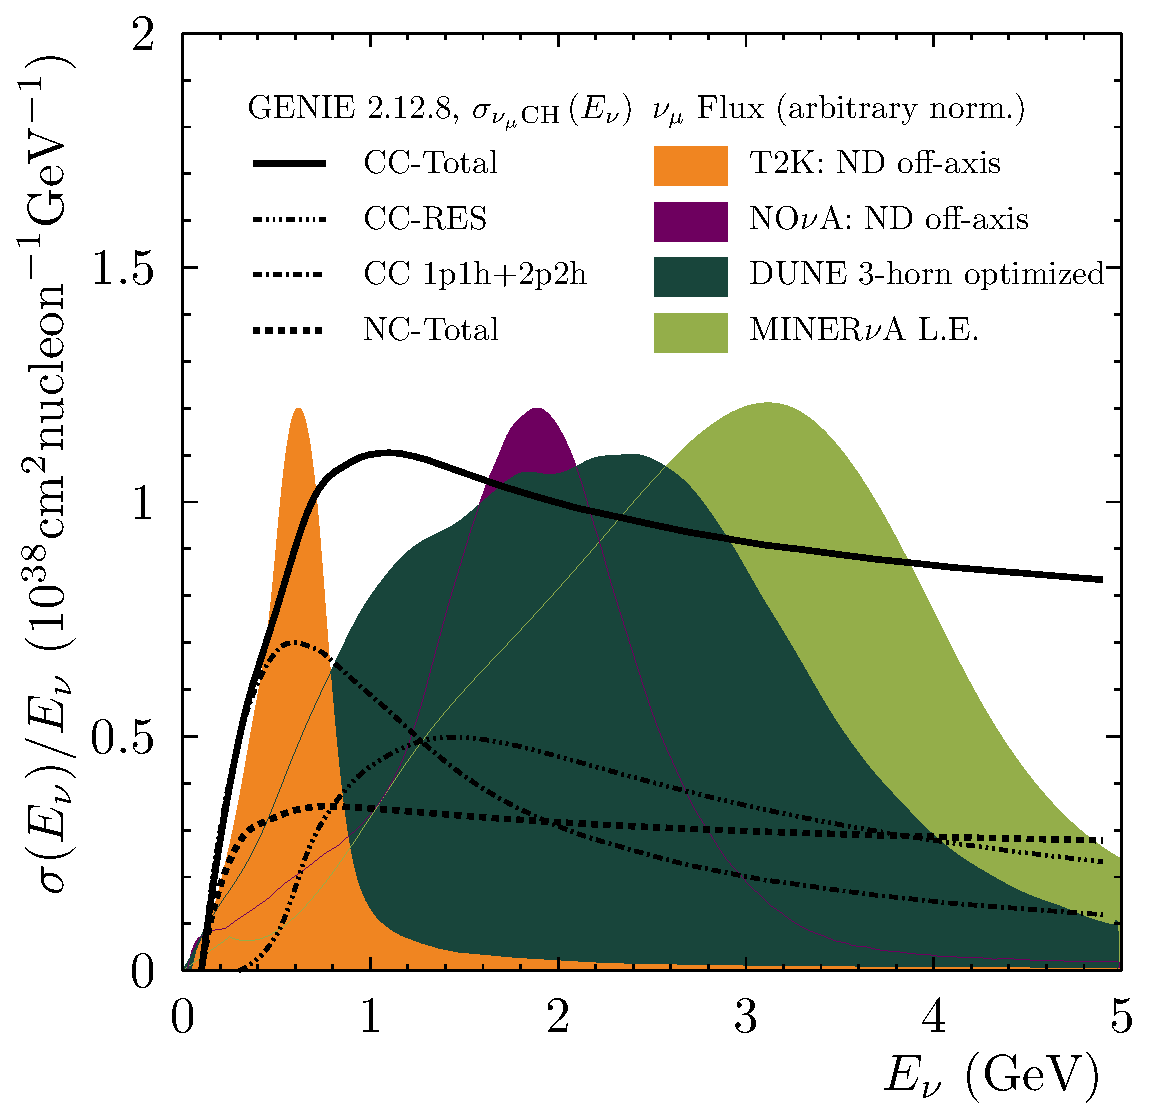
\includegraphics[width=\textwidth]{nu-detection/flux_and_xsec_from_luke}
	\caption{Neutrino interaction cross-section per nucleon as a function of neutrino energy in \si{\giga\electronvolt}.
	Overlaid are the flux shapes of various beam experiments in arbitrary units.
	The cross-section is split into contributions from charged (CC) and neutral current (NC) interactions.
	For CC, the individual contribution from resonant interactions (RES) is shown, as well as from the sum of 1p1h and 2p2h. The latter two correspond to the quasi-elastic channel and interactions involving meson exchange currents, respectively.}
	\todo[inline]{sauce}
	\label{fig:nu-detection_xsec}
\end{figure}

To better understand the meaning of Figure~\ref{fig:nu-detection_xsec}, a brief explanation of the cross-section concept is given here.
For a beam consisting of particles $A$, incident on a target made of particles $B$, the rate of the interaction $AB \rightarrow X$ is given by
\begin{IEEEeqnarray}{rCl}
	R_X & = & \phi_A N_B \sigma_{ABX} \qc
\end{IEEEeqnarray}
where $\phi_A$ is the flux of beam particles, $N_B$ is the number of target particles, and $\sigma_{ABX}$ is the cross-section.
Therefore, the cross-section
\begin{IEEEeqnarray}{rCl}
	\sigma_{ABX} & = & \frac{R_X}{\phi_A N_B}
\end{IEEEeqnarray}
is a measure for the interaction rate $R_X$ normalised by the number of both, beam and target, particles.
As flux is given in units of inverse time and area, and interaction rate in inverse time, the cross-section needs to have the dimension of an area.


\section{Final State Detection}
\label{sec:nu-detection_fs}

In order to be able to detect particles, they need to interact with a detection medium.
This section will describe the most important interaction of charged particles as well as neutral particles with matter.
A special focus is laid on charged interactions as these are the most important ones for \lartpc{}s.
As a measure of the interaction strength, the energy loss per distance or stopping power $\dv{E}{x}$ is used.
Where not otherwise mentioned, this section is based on~\cite{grupen}.

The main interaction of charged particles with matter happens on atomic electrons.
That is why for most of these interactions, one needs to treat the interaction of electrons separately.
For all other charged particles, the stopping power is described by the Bethe-Bloch formula
\begin{IEEEeqnarray}{rCl}
	- \frac{1}{\rho} \dv{E}{x} & = &
	4 \pi N_{\m{A}} r_{\m{e}} ^ 2 m_{\m{e}} c ^ 2 z ^ 2 \frac{Z}{A} \frac{1}{\beta ^ 2}
	\qty[\ln(\frac{2 m_{\m{e}} c ^ 2 \gamma ^ 2 \beta ^ 2}{I}) - \beta ^ 2 - \frac{\delta}{2}] \qc
	\label{eq:nu-detection_bethe-bloch}
\end{IEEEeqnarray}
where
\begin{description}
	\item[$\rho$] is the density of the absorber material,
	\item[$N_{\m{A}}$] is Avogadro's number,
	\item[$r_{\m{e}} = \frac{1}{4 \pi \varepsilon_{\m{0}}} \frac{\si{\elementarycharge} ^ 2}{m_{\m{e}} c ^ 2}$] is the classical electron radius using the permittivity of free space $\varepsilon_{\m{0}}$,
	\item[$m_{\m{e}}$] is the electron mass,
	\item[$z$] is the charge of the incident particle,
	\item[$Z$] is the atomic number of the absorber,
	\item[$A$] is the atomic weight of the absorber,
	\item[$\beta = \frac{v}{c}$] with $v$ the velocity of the incident particle,
	\item[$\gamma = \frac{E}{m_0 c ^ 2}$] with $E$ the energy and $m_0$ the rest mass of the incident particle,
	\item[$I$] is the mean excitation energy of the absorber material which can be approximated by
		\begin{IEEEeqnarray}{rCl}
			I & = & 16 Z ^ {0.9} \si{\electronvolt} \quad \m{for} \quad Z > 1 \qc
		\end{IEEEeqnarray}
	\item[$\delta$] is a parameter describing the screening of the extended transverse electric field of relativistic incident particles by the charge density of the atomic electrons of the absorber.
\end{description}
Equation~\eqref{eq:nu-detection_bethe-bloch} describes the stopping power of particles with $m_0 \gg m_{\m{e}}$ by ionisation and excitation of the atoms in the absorber material.
As the stopping power is proportional to the electron density and thus to the mass density of the absorber material, it is often divided by the latter.
Thus, Equation~\eqref{eq:nu-detection_bethe-bloch} actually gives the so called mass stopping power.
The only remaining dependence on the absorber material is $\frac{Z}{A}$ which is $\approx 0.5$ for most light materials, and the mean excitation energy which only contributes logarithmically.

\begin{figure}[htbp]
	\centering
	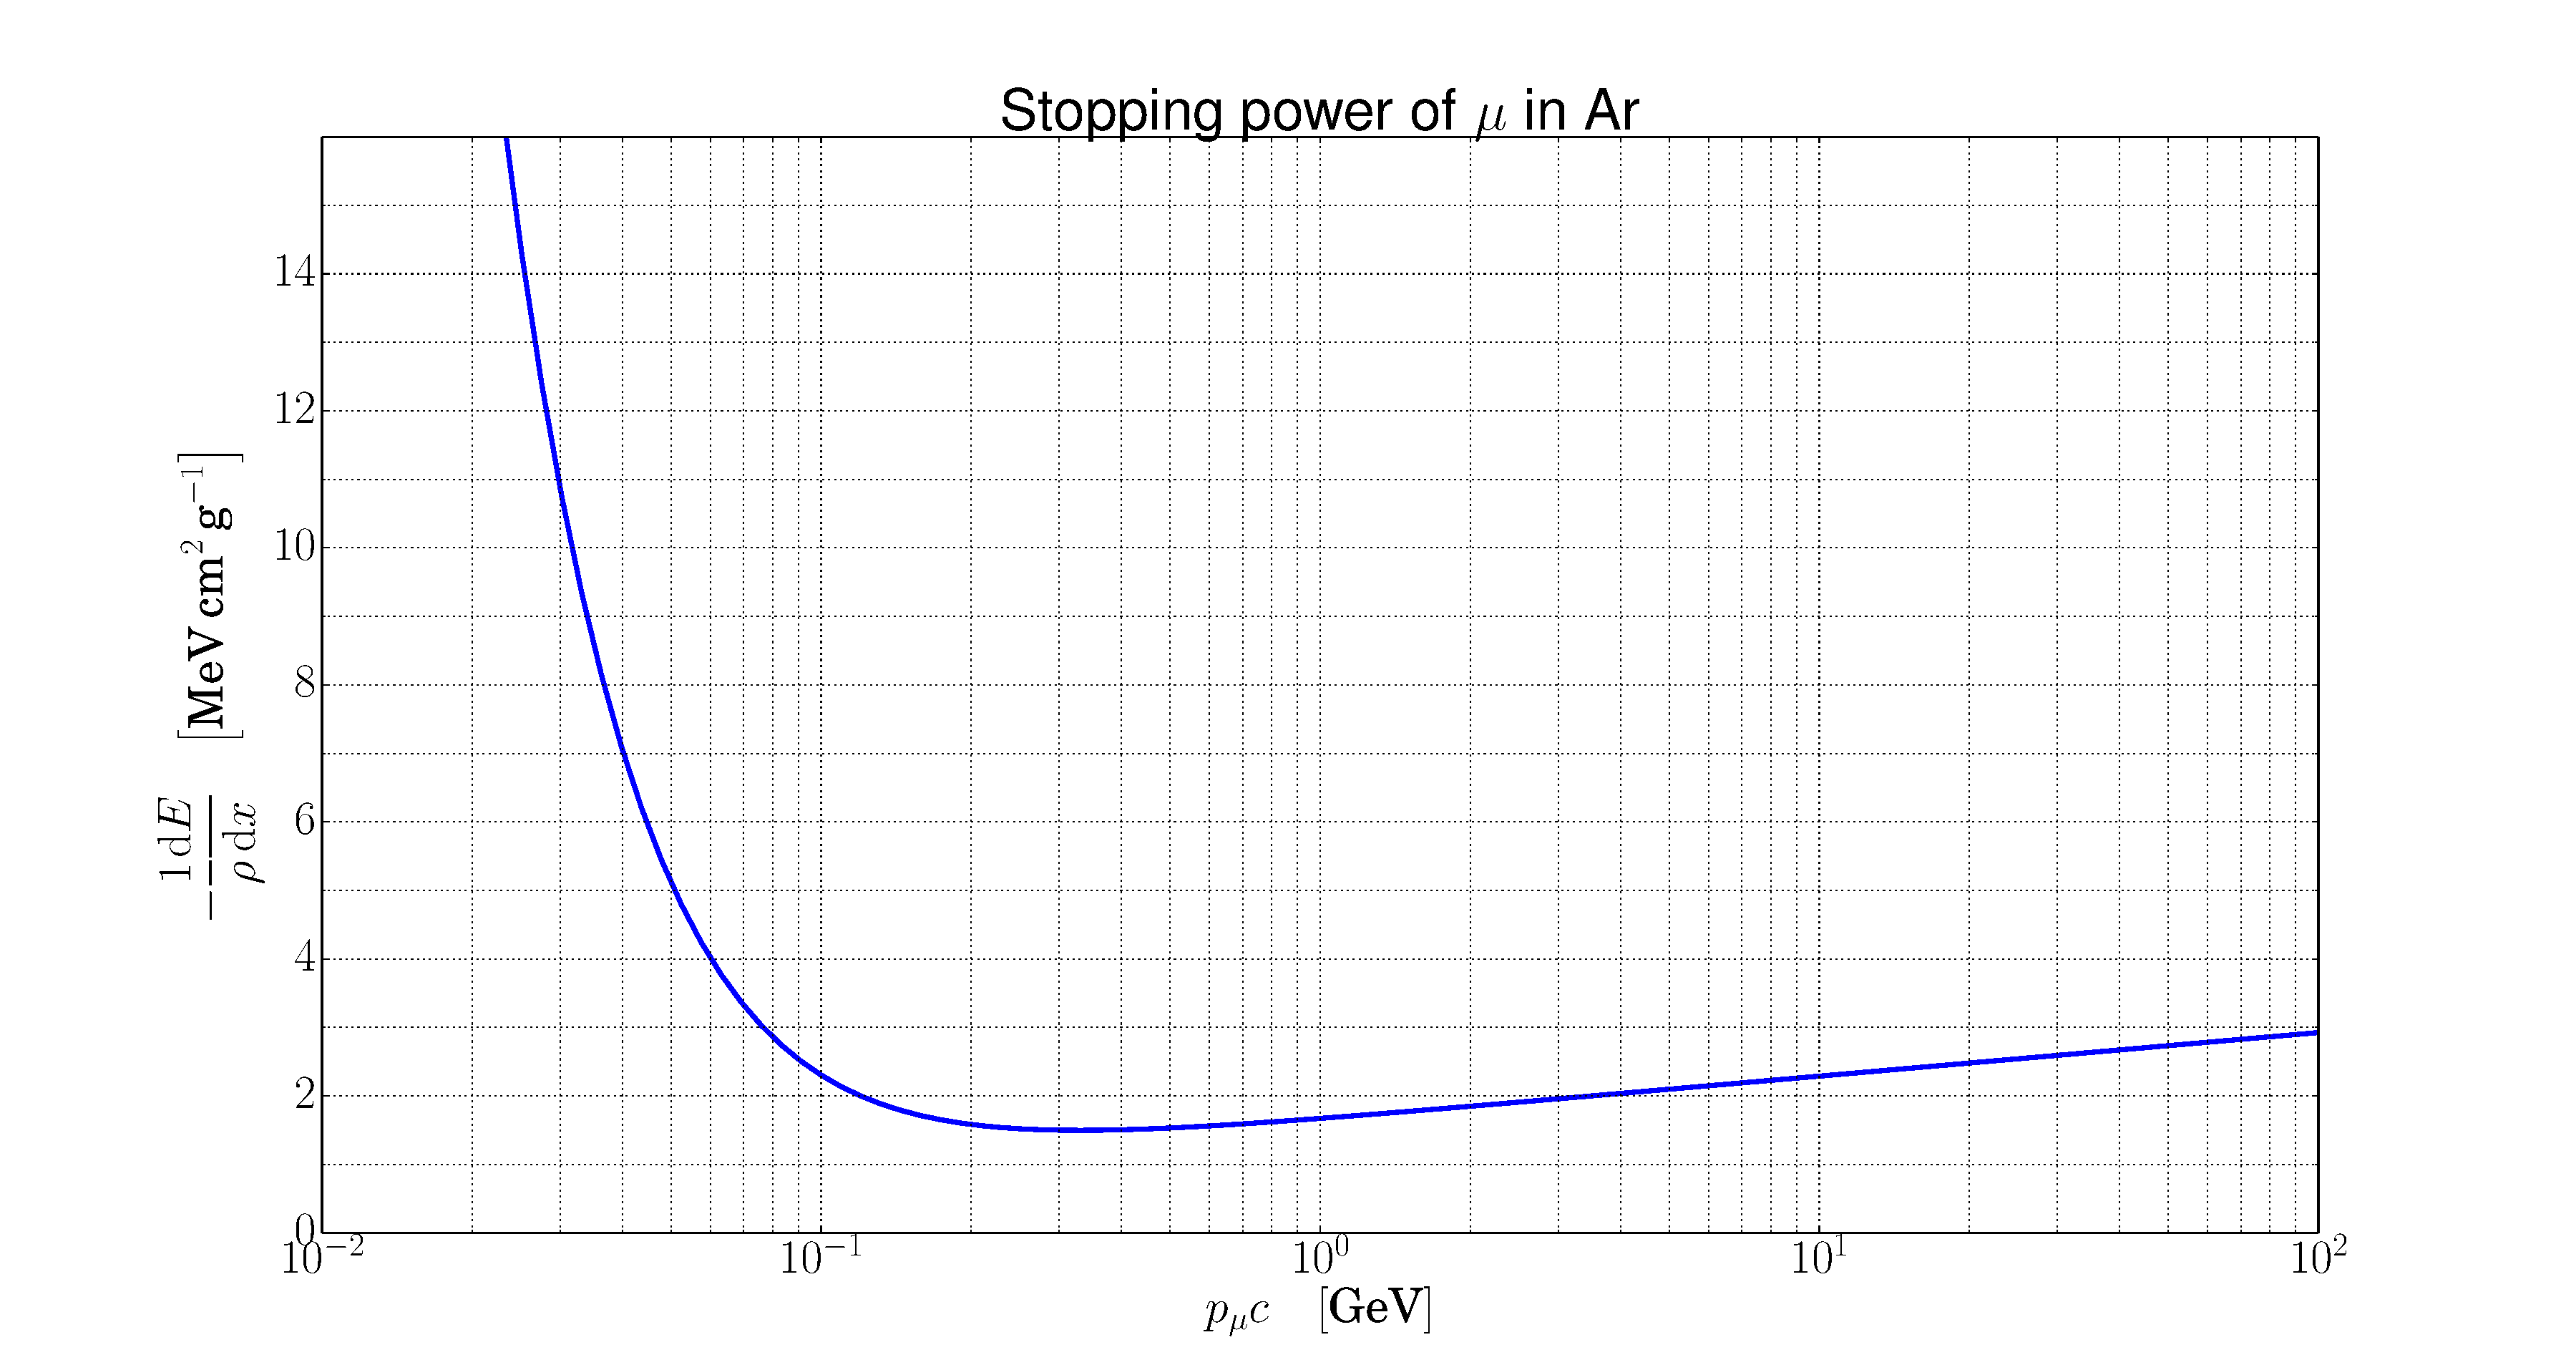
\includegraphics[width=\textwidth]{nu-detection/bethe-bloch}
	\caption{Bethe-Bloch stopping power of $\mu$ in \ce{Ar}}
	\todo[inline]{check}
	\label{fig:nu-detection_bethe-bloch}
\end{figure}

Figure~\ref{fig:nu-detection_bethe-bloch} shows the mass stopping power of $\mu$ in \ce{Fe} neglecting the $\frac{\delta}{2}$ term.
As can be seen, there is a broad minimum which is characteristic of the Bethe-Bloch formula.
Particles in this momentum range are called minimum ionising particles (MIPs).
They are important for detectors because this energy loss is a measure for the required energy resolution of a detector.
As mentioned above, the mass stopping power only loosely depends on the absorber material and therefore, its minimum is
\begin{IEEEeqnarray}{rCl}
	\eval{- \frac{1}{\rho} \dv{E}{x}}_{\m{min}} & \approx & \SI{2}{\mega\electronvolt\centi\meter\squared\per\gram}
\end{IEEEeqnarray}
for singly charged incident particles on most (light) absorbers.
To the left of the minimum is the \emph{Bragg peak} which is especially important for radiation therapy with heavy charged particles (e.g.\ protons).
The Bragg peak falls off with a strong $\frac{1}{\beta ^ 2}$ dependence.
After the minimum, the stopping power rises again with a logarithmic dependence on $\beta$ and the mean excitation energy of the absorber $I$.
The reason for this so called \emph{logarithmic rise} is the extension of the transverse electric field of the incident particle in the relativistic regime.
Due to increasing shielding of the transverse electric field by the shell electrons of the absorber materials, taken into account by the $\frac{\delta}{2}$ term, the rise is only asymptotic.
For electrons and positrons, Equation~\eqref{eq:nu-detection_bethe-bloch} does not hold because their mass is equal to the mass of the atomic electrons of the absorber.
The stopping power changes further for electrons because the incident particle cannot be distinguished form its collision partner in that case.
On the other hand, a positron will be annihilated upon stop by an electron which needs to be taken into account as well.
The equivalent of Equation~\eqref{eq:nu-detection_bethe-bloch} for $e^{\pm}$ can be found in~\cite{grupen}.

At high velocities, further effects come into play.
\emph{Bremsstrahlung} describes the radiation energy loss of a fast charged particle in the Coulomb field of the absorber nuclei.
It can be described by
\begin{IEEEeqnarray}{rCl}
	- \frac{1}{\rho}\dv{E}{x} & = & \frac{E}{X_{\m{0}}}
	\label{eq:nu-detection_bremsstrahlung}
\end{IEEEeqnarray}
where
\begin{IEEEeqnarray}{rCl}
	X_{\m{0}} & = & \frac{A}{4 \alpha N_A Z \qty(Z + 1) \qty(\frac{1}{4 \pi \varepsilon_{\m{0}}} \frac{\si{\elementarycharge} ^ 2}{m c ^ 2}) ^ 2 \ln(183 Z ^ {- \frac{1}{3}})}
	\label{eq:nu-detection_radiationlength}
\end{IEEEeqnarray}
is the \emph{radiation length} of the absorber material using
\begin{itemize}
	\item[$\alpha$] $\approx \frac{1}{137}$ the fine-structure constant and
	\item[$m$] the mass of the incident particle.
\end{itemize}
Again, the energy loss is proportional to the density of the absorber and for convenience, divided by the latter.
Bremsstrahlung is emitted in interactions of the incident particle with the absorber nuclei ($\propto Z ^ 2$) as well as with the atomic electrons of the absorber ($\propto Z$).
By neglecting the latter, one obtains the important relation
\begin{IEEEeqnarray}{rCl}
	X_0 ^ {- 1} & \propto & Z ^ 2
\end{IEEEeqnarray}
as opposed to the $\propto Z$ dependence of the Bethe-Bloch formula.
Equation~\eqref{eq:nu-detection_bremsstrahlung} also holds for electrons as long as $E \gg \frac{m_{\m{e}} c ^ 2}{\alpha Z ^ {\frac{1}{3}}}$.
Furthermore, looking at the dependence on the mass of the incident particle, one finds
\begin{IEEEeqnarray}{rCl}
	X_0 & \propto & m ^ 2
\end{IEEEeqnarray}
using Equation~\eqref{eq:nu-detection_radiationlength}.
Therefore, the radiation length of an absorber material is usually given for electrons and the relation
\begin{IEEEeqnarray}{rCl}
	X_0 & = & X_0^{\m{e}} \frac{m ^ 2}{m_{\m{e}} ^ 2}
\end{IEEEeqnarray}
can be used to get the radiation length for any charged particle of mass $m$.
Radiation losses play a significant role only at energies much higher than the energy of MIPs.
Using Equations~\eqref{eq:nu-detection_bethe-bloch} and~\eqref{eq:nu-detection_bremsstrahlung}, one can define a \emph{critical energy} $E_{\m{c}}$ by
\begin{IEEEeqnarray}{rCl}
	\eval{\dv{E}{x}_{\m{ion}}}_{E_{\m{c}}} & = & \eval{\dv{E}{x}_{\m{brems}}}_{E_{\m{c}}}
	\label{eq:nu-detection_ec}
\end{IEEEeqnarray}
at which radiation losses take over from ionisation losses.
Similar to the radiation length, the critical energy is proportional to $m ^ 2$.
Thus, it is most important for electrons while for other particles it becomes significant only at very high energies.
If we take the example of an iron absorber again for instance, we get $E_c^{\m{e}} = \SI{20.7}{\mega\electronvolt}$ and $E_c^{\mu} = \SI{890}{\giga\electronvolt}$.

At high energies, there are additional types of radiation loss taking place, for instance direct electron-pair production and photonuclear interactions.
They shall not be described here.
Instead, only their $\propto E$ relation similar to bremsstrahlung losses shall be mentioned.
A description of those effects can be found in~\cite{grupen}.

In addition to the processes described above, charged particles traversing matter also undergo scattering in the Coulomb field of the nuclei of the traversed medium.
Accordingly, this process is called \emph{multiple Coulomb scattering} or MCS.
The root mean square of the \emph{scattering-angle distribution}
\begin{IEEEeqnarray}{rCl}
	\Theta_{\m{RMS}} & = & \frac{\SI{13.6}{\mega\electronvolt}}{\beta c p} z \sqrt{\frac{2 x}{X_{\m{0}}}} \qty[1 + 0.038 \ln(\frac{x}{X_{\m{0}}})]
	\label{eq:nu-detection_highland}
\end{IEEEeqnarray}
is defined by the momentum $p$, velocity $\beta c$ and charge $z$ of the scattered particle, and the thickness of the scattering medium $\frac{x}{X_{\m{0}}}$ in radiation lengths.
The distinct momentum dependence of this so-called \emph{Highland formula} can be used to reconstruct the momentum of the incident particle provided the angular resolution of the detector is fine enough.

Concerning the interactions of charged particles with matter, there is one important note regarding detectors.
While charge produced in interactions (i.e.\ ionisation) can be detected directly, light (i.e.\ excitation photons and photon radiation) first needs to be converted to charge to be detected.
This conversion from light to electric charge is the topic of the next section.

Photons can interact with matter in different ways.
In particular, they can be converted to charge which can be detected.
The three most important interactions converting photons to charge shall be outlined in this section.
All of them have in common that they attenuate photon beams exponentially according to
\begin{IEEEeqnarray}{rCl}
	I & = & I_0 \m{e} ^ {- \mu x}
\end{IEEEeqnarray}
where $I_0$ and $I$ is the intensity before and after passing the absorber, respectively.
The thickness of the absorber is given by $x$ and
\begin{IEEEeqnarray}{rCl}
	\mu & = & \frac{N_A}{A} \sum_i \sigma_i
	\label{eq:nu-detection_mass-att-coeff}
\end{IEEEeqnarray}
is the \emph{mass attenuation coefficient} defined by the sum of the cross sections $\sigma_i$ of the different interaction processes.

At low energies (ionisation energy $\le E_{\gamma} \le \SI{100}{\kilo\electronvolt}$), photons primarily undergo conversion to charge by the \emph{photoelectric effect}.
The photon is absorbed by an atom of the absorber which in turn is ionised and thus ejects one of its shell electrons.
The cross section is given by
\begin{IEEEeqnarray}{rCl}
	\sigma_{\m{photo}} & = & \qty(\frac{32}{\epsilon ^ 7}) ^ \frac{1}{2} \alpha ^ 4 Z ^ 5 \sigma_{\m{Th}}^{\m{e}}
\end{IEEEeqnarray}
where
\begin{itemize}
	\item[$\epsilon$] $= \frac{E_{\m{\gamma}}}{m_{\m{e}} c ^ 2}$ is the reduced photon energy and
	\item[$\sigma_{\m{Th}}^{\m{e}}$] $= \frac{8}{3} \pi r_{\m{e}} ^ 2 = \SI{6.65e-25}{\centi\meter\squared}$ is the \emph{Thomson cross section} for elastic scattering of photons on electrons.
\end{itemize}

For energies $\approx \SI{1}{\mega\electronvolt}$, \emph{Compton scattering} dominates the interaction of photons with matter.
Thereby, the photon is not absorbed by the atom but just scatters off one of its shell electrons with the cross section
\begin{IEEEeqnarray}{rCl}
	\sigma_{\m{c}} & = & 2 \pi r_{\m{e}} ^ 2 Z \left\{\qty[\frac{1 + \epsilon}{\epsilon ^ 2}] \qty[\frac{2 \qty(1 + \epsilon)}{1 + 2 \epsilon} - \frac{1}{\epsilon} \ln(1 + 2 \epsilon)]\right.\\
	& & \left. + \frac{1}{2 \epsilon} \ln(1 + 2 \epsilon) - \frac{1 + 3 \epsilon}{\qty(1 + 2 \epsilon) ^ 2}\right\}
\end{IEEEeqnarray}
obtained from the Klein-Nishina formula.
As only part of the photon's energy is absorbed while the rest is scattered, it makes sense to divide this cross section into a scattering cross section
\begin{IEEEeqnarray}{rCl}
	\sigma_{\m{cs}} & = & \frac{E_{\gamma}'}{E_{\gamma}}
\end{IEEEeqnarray}
and an absorption cross section
\begin{IEEEeqnarray}{rCl}
	\sigma_{\m{ca}} & = & \sigma_{\m{c}} - \sigma_{\m{cs}}
	\label{eq:nu-detection_sigma-compton}
\end{IEEEeqnarray}
where $E_{\gamma}$ and $E_{\gamma}'$ is the energy of the photon before and after scattering, respectively.

At $E_{\gamma} \ge 2 m_{\m{e}} c ^ 2$, photons are capable of producing pairs of $e^+ e^-$.
Because of momentum conservation, this process can only happen in the coulomb field of a so called spectator particle.
As pair-production in the field of an electron is strongly suppressed, the spectator is usually a nucleus of the absorber material.
Therefore, the cross section of pair-production depends on the shielding of the coulomb field by the shell electrons and thus on the proximity to the nucleus.
Eventually, this results in an energy dependence.
For $1 \ll \epsilon < \frac{1}{\alpha Z ^ {\frac{1}{3}}}$, the cross section is given by
\begin{IEEEeqnarray}{rCl}
	\sigma_{\m{pair}} & = & 4 \alpha r_{\m{e}} ^ 2 Z ^ 2 \qty(\frac{7}{9} \ln 2 \epsilon - \frac{109}{54})
\end{IEEEeqnarray}
and for $\epsilon \gg \frac{1}{\alpha Z ^ {\frac{1}{3}}}$, the cross section is
\begin{IEEEeqnarray}{rCl}
	\sigma_{\m{pair}} & = & 4 \alpha r_{\m{e}} ^ 2 Z ^ 2 \qty[\frac{7}{9} \ln(\frac{183}{Z ^ {\frac{1}{3}}}) - \frac{1}{54}] \qq*{.}
\end{IEEEeqnarray}

As mentioned above, for Compton scattering, two different cross sections are defined, $\sigma_{\m{cs}}$ for the scattered energy and $\sigma_{\m{ca}}$ for the absorbed energy.
Consequentially, there are also different definitions of the coefficient $\mu$ in Equation~\eqref{eq:nu-detection_mass-att-coeff}.
Replacing the total Compton cross section $\sigma_{\m{c}}$ by $\sigma_{\m{ca}}$ from Equation~\eqref{eq:nu-detection_sigma-compton}, one gets the \emph{mass absorption coefficient} $\mu_{\m{a}}$, only taking into account photon absorption processes.
While $\mu$ is more precisely called the \emph{total mass attenuation coefficient}.

An interesting effect takes place for $e^{\pm}$ traversing material at energies higher than the critical energy $E_{\m{c}}$ defined by Equation~\eqref{eq:nu-detection_ec}.
In this regime, the energy loss is dominated by bremsstrahlung for $e^{\pm}$ and by pair production for $\gamma$.
This leads to an \emph{electromagnetic (EM) cascade} or \emph{shower} where $e^{\pm}$ and $\gamma$ produce each other alternately in a self-sustaining process.
The mean free path of a $\gamma$ before pair production
\begin{IEEEeqnarray}{rCl}
	\lambda_{\m{prod}} & = & \frac{9}{7}X_{\m{0}}
\end{IEEEeqnarray}
is very close to the mean free path of an $e^{\pm}$ before bremsstrahlung, the radiation length $X_{\m{0}}$.
Therefore, the number of particles participating in the shower doubles roughly every radiation length resulting in an exponential growth.
When the average energy per paticle drops below the critical energy, ionisation losses begin to dominate over radiative losses for $e^{\pm}$ and Compton and photoelectric effect over pair production for $\gamma$.
At this point, the shower reaches its maximum and
\begin{IEEEeqnarray}{rCl}
	t_{\m{max}} & = & \frac{\ln(\frac{E_{\m{0}}}{E_{\m{c}}})}{\ln(2)}
\end{IEEEeqnarray}
is its longitudinal extent in radiation lengths.
The \emph{Molière radius}
\begin{IEEEeqnarray}{rCl}
	R_{\m{M}} & = & \frac{\SI{21}{\mega\electronvolt}}{E_{\m{c}}} X_{\m{0}}
\end{IEEEeqnarray}
is the transversal extent of the shower divided by the the material density.
Both $t_{\m{max}}$ and $R_{\m{M}}$ are important benchmarks for the dimensioning of electromagnetic calorimeters.
Naturally, a $\gamma$ in the energy range where pair production dominates will produce a shower as well.
On the other hand, also $\mu^{\pm}$ can start electromagnetic cascades, if there energy is high enough to produce bremsstrahlung.

Similarly, hadrons interacting with matter via the strong force can produce cascades as well.
As opposed to the electromagnetic showers governed only by $e^{\pm}$ and $\gamma$, the hadronic process is much more complex because many different secondary particle can be involved.
Hadrons start to shower because they mainly interact inelastically with matter, producing secondary strongly interacting particles.
That is why the hadronic cross-section
\begin{IEEEeqnarray}{rCl}
	\sigma_{\m{total}} & = & \sigma_{\m{elastic}} + \sigma_{\m{inel}}
\end{IEEEeqnarray}
is usually split.
From $\sigma_{\m{inel}}$, one can derive the \emph{interaction length}
\begin{IEEEeqnarray}{rCl}
	\lambda_{\m{I}} & = & \frac{A}{N_{\m{A}} \rho \sigma_{\m{inel}}}
\end{IEEEeqnarray}
which describes the absorption of hadrons in matter according to
\begin{IEEEeqnarray}{rCl}
	N & = & N_{\m{0}} e ^ {- \frac{x}{\lambda_{\m{I}}}}
\end{IEEEeqnarray}
with the initial number of hadrons $N_{\m{0}}$ and number of hadrons $N$ after a distance $x$ of absorber material.
For absorbers with $Z \geq 6$, the interaction length is much larger than the radiation length $X_{\m{0}}$ meaning that hadronic calorimeters usually need to be much larger than their electromagnetic counterparts.
\chapter{The liquid argon time projection chamber (LArTPC)\label{chap:lartpc}}
The time projection chamber (TPC) is a derivative of Charpak's multi-wire proportional chamber (MWPC)\cite{mwpc} developed by Nygren in 1968~\cite{sauce}.
Passing charged particles ionise the detection medium which was gaseous in the original design.
To prevent the recombination of the ions and electrons, an electric field is applied.
In this field, the electrons drift towards a two-dimensional readout plane.
Originally, the readout was an MWPC.
The charge readout is triggered by a scintillation light readout which also provides accurate timing of an event.
Using this, one can measure the time for the ionisation time to reach the readout plane.
Because the drift speed of charged particles in the detection medium is constant, the coordinate in drift direction can be calculated from the drift time if the drift speed is known.

While gaseous TPCs already provide very accurate tracking, they have the disadvantage that the mass and thus the cross-section of the detection medium is quite low resulting in a low interaction rate.
Therefore, Rubbia in 1977 proposed to use liquid argon as a detection medium~\cite{lartpc}.
In turn, this requires a cryogenic detector while gaseous detectors can be operated at room temperature.


\section{Liquid argon as a detection medium\label{sec:lartpc_lar}}
\begin{itemize}
	\item General specs
	\item Electronegativity
	\item Ionisation
	\item Scintillation
	\item Recombination
	\item Diffusion
	\item Dielectric strength
\end{itemize}
\cite{NobleGasDetectors}


\section{Electric field generation\label{sec:lartpc_efield}}
For charge separation and drift, an electric field of the order of \SI{1}{\kilo\volt\per\centi\metre} is needed inside the fiducial volume of a LArTPC.
An easy way to achieve this is by means of field shaping rings fed by a resistive divider between cathode and anode.
The drawback is the need for a feedthrough capable of withstanding the full cathode voltage.
One alternative is to generate the high voltage inside the cryostat, for instance using a Greinacher voltage multiplier circuit as the one used for the ARGONTUBE experiment at LHEP at the University of Bern~\cite{AT}.
A Greinacher multiplier works by pumping up a cascade of capacitors and diodes using a high frequency source.
However, while the voltage generation itself worked well, this approach proofed to be impractical because the high frequency voltage needed to charge the multiplier interfered with the readout and therefore had to be turned off during data-taking.
Recharging, in turn, caused a lot of detector down time.


\section{Charge readout\label{sec:lartpc_readout}}
Classically, the charge readout of a liquid argon TPC is done using wires with a diameter of the order of \SI{100}{\micro\metre}.
One wire plane delivers a 2D projection of the ionisation tracks in the detection medium.
This has two consequences:
\begin{enumerate}
	\item At least two parallel wire planes are needed to be able to reconstruct the 3D event topology.
	\item In theory, the higher the complexity of the event, the more planes would be required to be able to fully reconstruct it.
\end{enumerate}
Multiple wire planes can be realised by operating only the last one (in drift direction) in charge collection mode.
All the preceeding wire planes are biased in a such a way that they are transparent to the incoming charge but pick up an induction signal during the passage of the latter.
A typical number of wire planes for currently operational detectors is three.
They are tilted by \SI{60}{\degree} against each other.


\section{Light readout\label{sec:lartpc_light}}


\section{Electronics\label{sec:lartpc_electronics}}


\section{Challenges of future detectors\label{sec:lartpc_challenges}}
\chapter{High voltage studies}
\label{chap:hv}

The difficulties involved with the necessary voltages have been highlighted by the Bern Group’s work, in which I have already played a key role\cite{breakdown_16}.
For the first time, we took high speed footage of breakdowns in liquid argon, measured their current-voltage characterisitcs and recorded their optical spectral distribution.
These measurements help to understand the physics of the breakdowns and develop ways to mitigate them and/or protect future detectors from catastrophic failures.
Our HV studies have already influenced the design of \uboone{} and will continue to impact the design of future experiments.


\section{Experimental Setup}
\label{sec:hv_setup}

\begin{figure}[htb]
	\centering	
	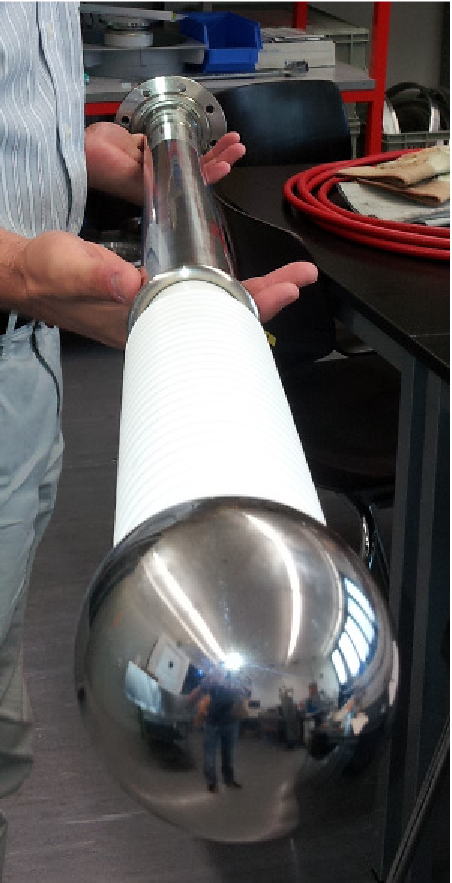
\includegraphics[width=0.265\textwidth]{hv/FT}
	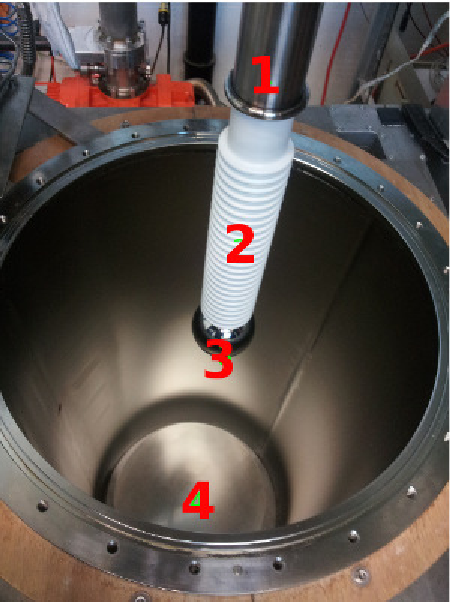
\includegraphics[width=0.39\textwidth]{hv/setup1_lowres}
	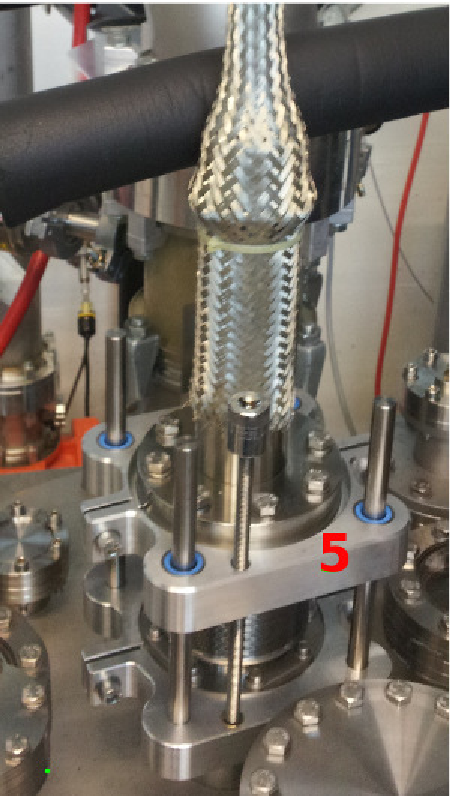
\includegraphics[width=0.295\textwidth]{hv/setup2_lowres}
	\caption{Experimental setup. Left: high voltage feed-through with the spherical cathode. Middle: the feed-through before insertion into the cryostat. 1.~ground shield of the feed-through; 2.~ribbed PET dielectric; 3.~cathode sphere; 4.~anode plate sitting on a tripod on the grounded bottom of the cryostat; two of the tripod legs are insulated while the third one contains a \SI{50}{\ohm} shunt resistor. Right: linear translation unit used to set the cathode-anode gap width~(5).}
	\label{fig:hv_setup1}
\end{figure}

The setup used in this study is very similar to the one described in~\cite{breakdown_14} and is shown in Figure~\ref{fig:hv_setup1}.
A spherical cathode and a plane anode electrode form the discharge gap.
Three different diameters of the cathode sphere were tested: \SIlist{4; 5; 8}{\centi\metre}.
Two types of surface treatment were used in the cathode preparation, namely mechanical fine polishing and electro-polishing.
For the anode, mechanical fine polishing was used for all measurements.
The anode-cathode gap width can be set in the range of \SI{0}{\milli\metre} to \SI{100}{\milli\metre} with a precision of \SI{0.3}{\milli\metre}.
An example of the field distribution in the setup is shown in Figure~\ref{fig:hv_efield}.
The field map was calculated using the COMSOL FEM package.\footnote{\url{http://www.comsol.com}}

\begin{figure}[htb]
	\centering	
	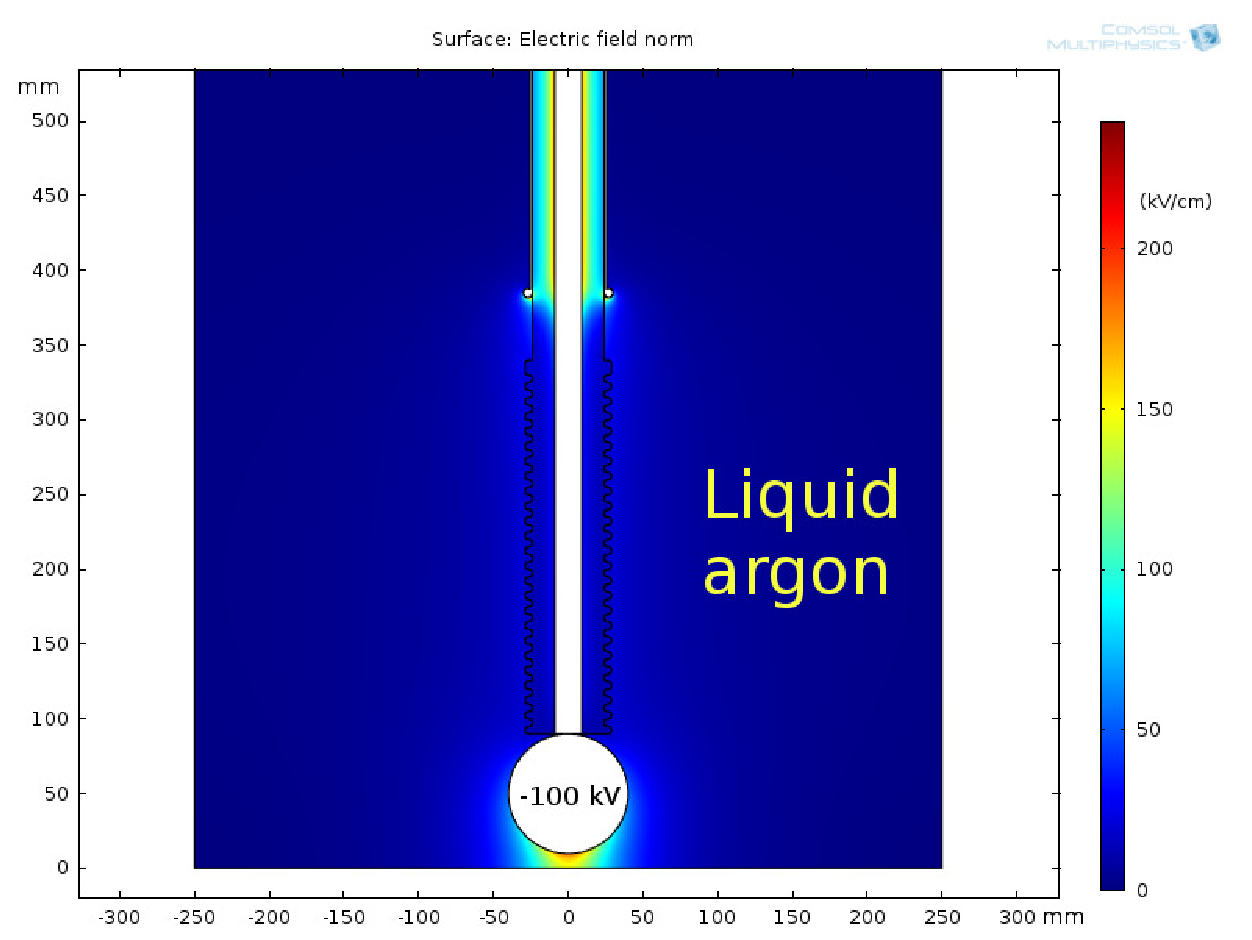
\includegraphics[width=\textwidth]{hv/EField}
	\caption{Calculated electric field-amplitude map for the test setup with \SI{-100}{\kilo\volt} at the cathode and cathode-anode distance of \SI{1}{\centi\metre}.}
	\label{fig:hv_efield}
\end{figure}

The purity of the argon after filling was estimated with a small time projection chamber (according to the method described in~\cite{2photonAbs}) to be of the order of \SI{1}{ppb} of oxygen-equivalent impurity concentration.
More details of the setup can be found in~\cite{breakdown_14}.

The control circuit of the \emph{Spellman SL150}\footnote{\url{http://www.spellmanhv.com}} power supply unit (PSU) outputs two low voltages proportional to the voltage and the current at the output, respectively.
These voltages are recorded with a \emph{Tektronix DPO 3054}\footnote{\url{http://www.tek.com}} digital oscilloscope.
The output polarity of the PSU can be switched by replacing the output HV multiplier module.
To measure the discharge current, a \SI{50}{\ohm} shunt resistor is placed between the anode plate and the vessel ground which is connected to the ground return of the PSU. The voltage drop across the shunt resistor is transmitted via a matched coaxial line to the oscilloscope.
The latter is controlled by a LabVIEW program.
The equivalent electric scheme of the setup is shown in Figure~\ref{fig:hv_scheme}. 
The voltage at the $V_{\m{mon}}$ output of the power supply corresponds to the PSU output voltage divided by a factor $K_{\m{V}}$.
The voltage at $I_{\m{mon}}$ is related to the PSU output current.
However, according to the manufacturer of the PSU, an accurate reconstruction of the output current for frequencies above \SI{100}{\hertz} is not possible because of a filtering circuit in the current control loop.
Therefore, for the measurement of the discharge current only the voltage drop across the shunt resistor is used.

\begin{figure}[htb]
	\centering
	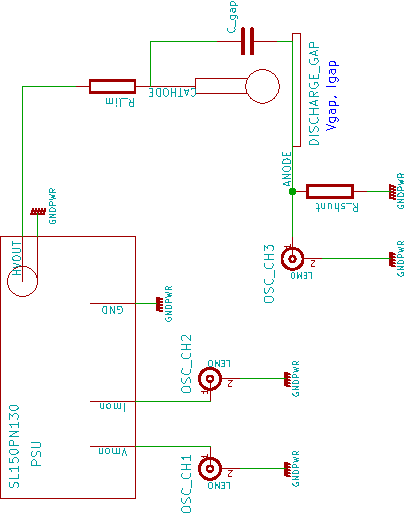
\includegraphics[width=0.7\textwidth]{hv/scheme}
	\caption{Electric scheme of the experimental setup. The oscilloscope is connected to the control circuit of the high voltage power supply and to a shunt resistor on the ground return path. From the recorded voltages, the voltage and the current of the discharge can be derived.}
	\label{fig:hv_scheme}
\end{figure}

The oscilloscope is triggered by the channel connected to the shunt resistor.
The breakdown discharge current is composed of the output current of the PSU and the discharge current of the setup capacitance $C_{\m{gap}}$ as $I_{\m{gap}} = I_{\m{out}} + C_{\m{gap}}\frac{\m{d}V_{\m{gap}}}{\m{d}t}$.
To limit the PSU output current an additional resistor R$_{lim}$ is inserted into the HV output circuit.
The measured values for the circuit parameters are summarized in Table~\ref{tab:hv_table1}.
The knowledge of these parameters allows to calculate the voltage across the gap during breakdown. 

\begin{table}[htb]
	\centering
	\caption{Summary of the measured parameters of the test circuit.}
	\label{tab:hv_table1}
	\begin{tabu} to \textwidth {|l|S|}
		\hline
		$K_{\m{V}}$ & 		42.3e-6 \\
		\hline
		$R_{\m{shunt}}$ &	\SI{50}{\ohm} \\
		\hline
		$R_{\m{lim}}$ & 	\SI{200}{\mega\ohm} \\
		\hline
		$C_{\m{gap}}$ & 	\SI{370}{\pico\farad} \\
		\hline
	\end{tabu}
\end{table}

In addition, the setup is equipped with an \emph{AOS Technologies S-PRI\emph{Plus}}\footnote{\url{http://www.aostechnologies.com}} high-speed camera to observe the development of the discharge. The camera is capable of recording \num{700 x 400}~pixel RGB images at \SI{1230}{fps}.
The camera comprises a frame ring buffer and is triggerable by an external TTL pulse.
This allows a synchronous recording of the visual appearance of the discharge and its volt-ampere characteristics.
The camera is triggered from the \emph{TRIG} output of the oscilloscope.
The luminous part of the discharge is analysed for each frame of the recorded sequence.

The camera is mounted above a \SI{5}{\centi\metre} diameter glass view port, located at the top flange of the cryostat and is looking downward.
To observe a discharge from the side, a glass mirror plate is installed at the edge of the cathode plane located \SI{20}{\centi\metre} from the cathode, in such a way as to not perturb the electric field in the discharge gap. 

Finally, a custom built optical spectrometer is used to analyze the light emission of the discharges.
The spectrometer is connected to an optical fiber entering the cryostat with its other end attached to the anode plate.
The fiber is aligned such that its end directly faces the discharge gap resulting in a high angular acceptance.
As will be shown later, the discharge emission spectra allow to better understand the processes at different stages of the discharge.
This is due to the fact that the emission spectra of excited neutral atomic argon, singly-ionized and multiply-ionized atoms lay in different regions of the visible spectrum.

The possibility of creating gas bubbles near the discharge gap is inhibited by keeping the pressure in the inner vessel at \SI{100}{\milli\bar} above atmospheric pressure, plus an additional \SI{100}{\milli\bar} due to the hydro-static pressure.
The outer bath is opened to the atmosphere, thus keeping the inner vessel temperature constant and well below the boiling point.
No boiling was detected anywhere near the discharge gap region during the measurements.


\section{Experimental Results}

\begin{figure}[htb]
	\centering	
	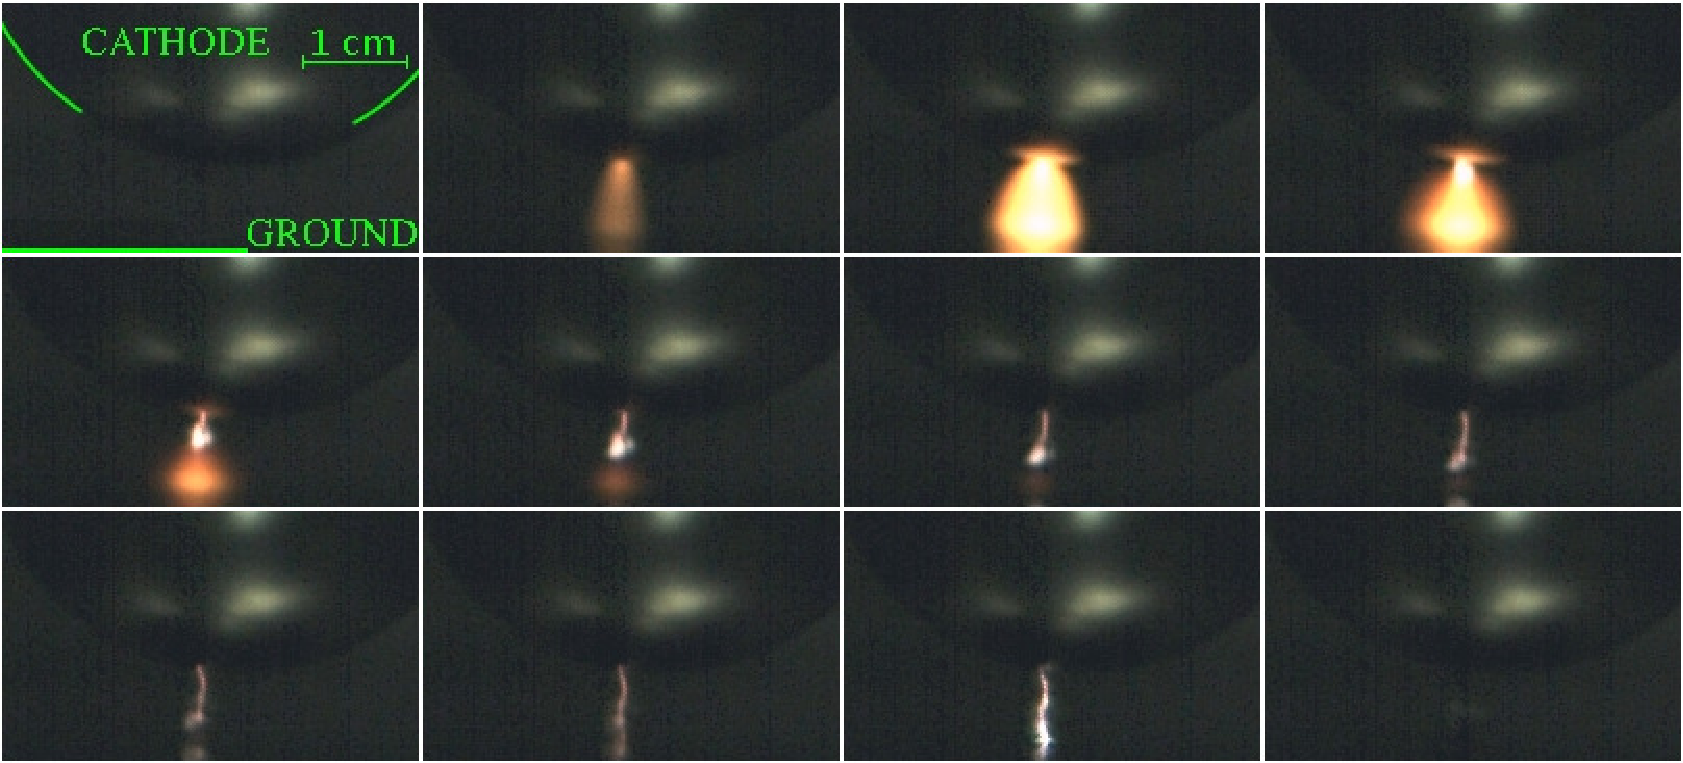
\includegraphics[width=\textwidth]{hv/montage}
	\caption{Recorded camera image sequence for a breakdown from a \SI{5}{\centi\metre} diameter cathode at \SI{-100}{\kilo\volt} and \SI{8.8}{\milli\metre} apart from the anode plate. The sequence is taken at \SI{1250}{fps}, each frame takes \SI{0.8}{\milli\second}.}
	\label{fig:hv_images}
\end{figure}

In earlier measurements~\cite{breakdown_14}, sporadic discharges were experienced across the ribs of the dielectric of the high voltage feed-through.
By rising the level of the liquid argon by about \SI{20}{\centi\metre}, it was possible to suppress these discharges completely.
This improved the cooling of the feed-through and reduced bubble production near the bottom of the feed-through grounded shield, placed \SI{60}{\centi\metre} below the liquid surface. 

The measurement campaign comprised \num{5}~runs with a total of more than \num{5000} measured discharges, with varying sphere diameter, surface treatment and polarity.
A summary is shown in Table~\ref{tab:hv_table2}.
A typical recorded camera image sequence for breakdown from a \SI{5}{\centi\metre} diameter cathode at \SI{-100}{\kilo\volt} and \SI{8.0}{\milli\metre} apart from the anode plate is shown in Figure~\ref{fig:hv_images}.
The movie can be found as \emph{movie1.webm} in the ancillary files of~\cite{breakdown_16}.\footnote{\url{http://arxiv.org/src/1512.05968v2/anc/movie1.webm}}

\begin{table}[htb]
	\centering
	\caption{Summary of the breakdown measurement runs.}
	\label{tab:hv_table2}
	\begin{tabu} to \textwidth {|S|S|X|X|S|S[range-units=brackets]|S[range-units=brackets]|}
		\hline
		{{Run}} &	{{$\varnothing_{\m{Sphere}}$}} &	Surface finish &	Sphere polarity &	{{Events}} &	{{$d_{\m{Gap}}$}} &					{{$V_{\m{Breakdown}}$}} \\
		\hline
		\hline
		1   &		\SI{4}{\centi\metre} &				Mech.\ polished &	Cathode ($-$) &		1086 &			\SIrange{0.5}{8.0}{\milli\metre} &	\SIrange{3}{130}{\kilo\volt} \\
		\hline
		2   &		\SI{5}{\centi\metre} &				Mech.\ polished &	Cathode ($-$) &		900 &			\SIrange{0.2}{12.0}{\milli\metre} &	\SIrange{2}{130}{\kilo\volt} \\
		\hline
		3   &		\SI{8}{\centi\metre} &				Mech.\ polished &	Cathode ($-$) &		2434 &			\SIrange{0.1}{70.0}{\milli\metre} &	\SIrange{1}{130}{\kilo\volt} \\
		\hline
		4   &		\SI{5}{\centi\metre} &				Mech.\ polished &	Anode ($+$) &		102 &			\SIrange{4.0}{5.0}{\milli\metre} &	\SIrange{5}{114}{\kilo\volt} \\
		\hline
		5   &		\SI{5}{\centi\metre} &				Electro-polished &	Cathode ($-$) &		1141 &			\SIrange{0.1}{10.0}{\milli\metre} &	\SIrange{1}{130}{\kilo\volt} \\
		\hline
	\end{tabu}
\end{table}

\begin{figure}[p]
	\centering
	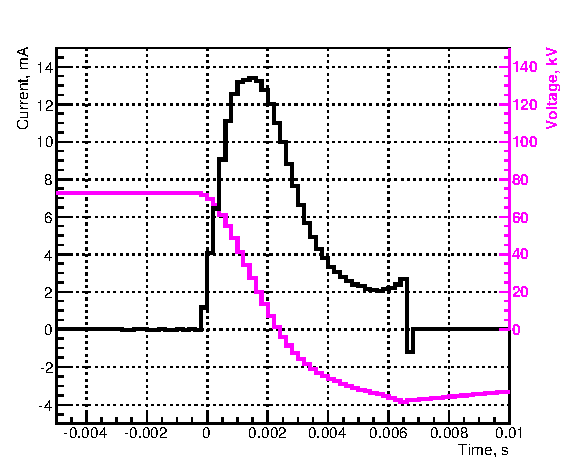
\includegraphics[height=0.43\textheight]{hv/IVuncorr}\\
	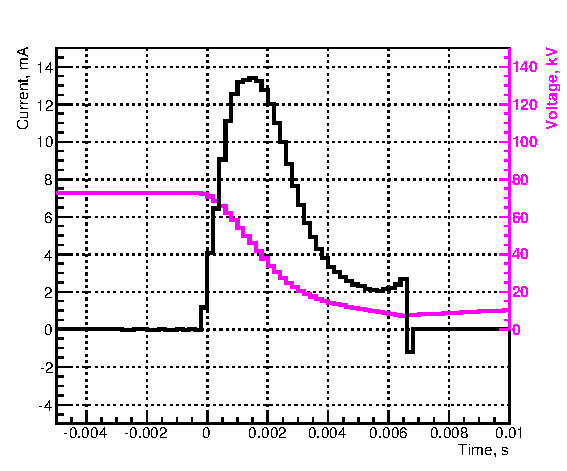
\includegraphics[height=0.43\textheight]{hv/IVcorr}
	\caption{Measured current through the gap (black) and voltage across the gap (magenta) for a typical breakdown at \SI{6.0}{\milli\metre} distance between a \SI{4}{\centi\metre} diameter cathode and the anode plate. The top plot shows the voltage obtained using the measured values of the protection resistor and the gap capacitance, while the bottom plot uses the tuned values.}
	\label{fig:hv_iv}
\end{figure}
\afterpage{\clearpage}

In Figure~\ref{fig:hv_iv}, the current and voltage features of a similar breakdown is shown from a \SI{4}{\centi\metre} diameter cathode at \SI{6.0}{\milli\metre} from the anode plate.
The current was directly measured by observing the voltage drop across the shunt resistor, while the voltage was obtained by integrating the current taking into account the gap capacitance, the protection resistor and the output voltage of the power supply.
When using the measured values of Table~\ref{tab:hv_table1} for capacitance and resistance, this results in a negative voltage at the end of most discharges.
This is an unphysical result as can be seen in the top plot of Figure~\ref{fig:hv_iv}.
This behavior may be attributed to poor knowledge of the effective values of the current-limiting resistor and the setup capacitance in the frequency domain of the discharge.
In order to better approximate these parameters, they are tuned in such a way that the minimum voltage for a maximum number of discharges approaches zero.
The best result was achieved by lowering the resistance by a factor of 1.7 and increasing the capacitance by the same factor.
Interestingly, this result leaves the RC characteristics of the system unchanged.
The bottom plot of Figure~\ref{fig:hv_iv} shows the result obtained by using the tuned values for capacitance and resistance.

Most of the discharges are localized in the area of high field concentration between the tip of the sphere and the anode plane.
However, in rare cases, the discharge is initiated far from that region, sometimes at the side surface of the sphere.
An example of such a discharge is shown in Figure~\ref{fig:hv_side} and the corresponding movie can be found as \emph{movie2.webm} in the ancillary files of~\cite{breakdown_16}.\footnote{\url{http://arxiv.org/src/1512.05968v2/anc/movie2.webm}}

\begin{figure}[htb]
	\centering	
	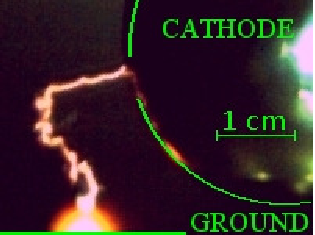
\includegraphics[width=.75\textwidth]{hv/sidespark}
	\caption{An image of the streamer stage of the discharge, initiated at the side surface of a \SI{5}{\centi\metre} cathode sphere at \SI{-121.5}{\kilo\volt} and \SI{8.0}{\milli\metre} apart from the anode plate. The cone of electrons emitted into liquid from the streamer tip towards the anode (lower edge of the image) produces bright orange luminescence in liquid argon.}
	\label{fig:hv_side}
\end{figure}


\section{Interpretation}

As it was shown in \cite{FNAL-hv-paper, he-breakdown}, experimental data on breakdowns in liquefied noble gases suggest the following dependence for the maximum field at the breakdown: $E_{max}=C\cdot A^p$, where $C$ is a material-dependent constant, $A$ is the stressed area with an electric field intensity above \SI{90}{\percent} of its maximum, and $p\approx-0.25$.
In Figure \ref{fig:hv_powerplot}, data available in literature is combined with those obtained from the measurements performed within the scope of this thesis as well with earlier measurements performed at LHEP at the University of Bern.
Each data point is the mean value of all measurements of one run taken at the same gap distance and therefore with the same stressed area.
The global best fit gives the following values for the parameters: $C = \num{139 +- 5}$ and $p = \num{-0.22 +- 0.01}$.
The statistical uncertainties represented by the error bars (smaller than the marker where not shown) are small compared to the unknown systematic uncertainties.
Indications for this are the high spread of the points around the fit line and the high reduced chi-square of \num{7283}.

\begin{figure}[htb]
	\centering
	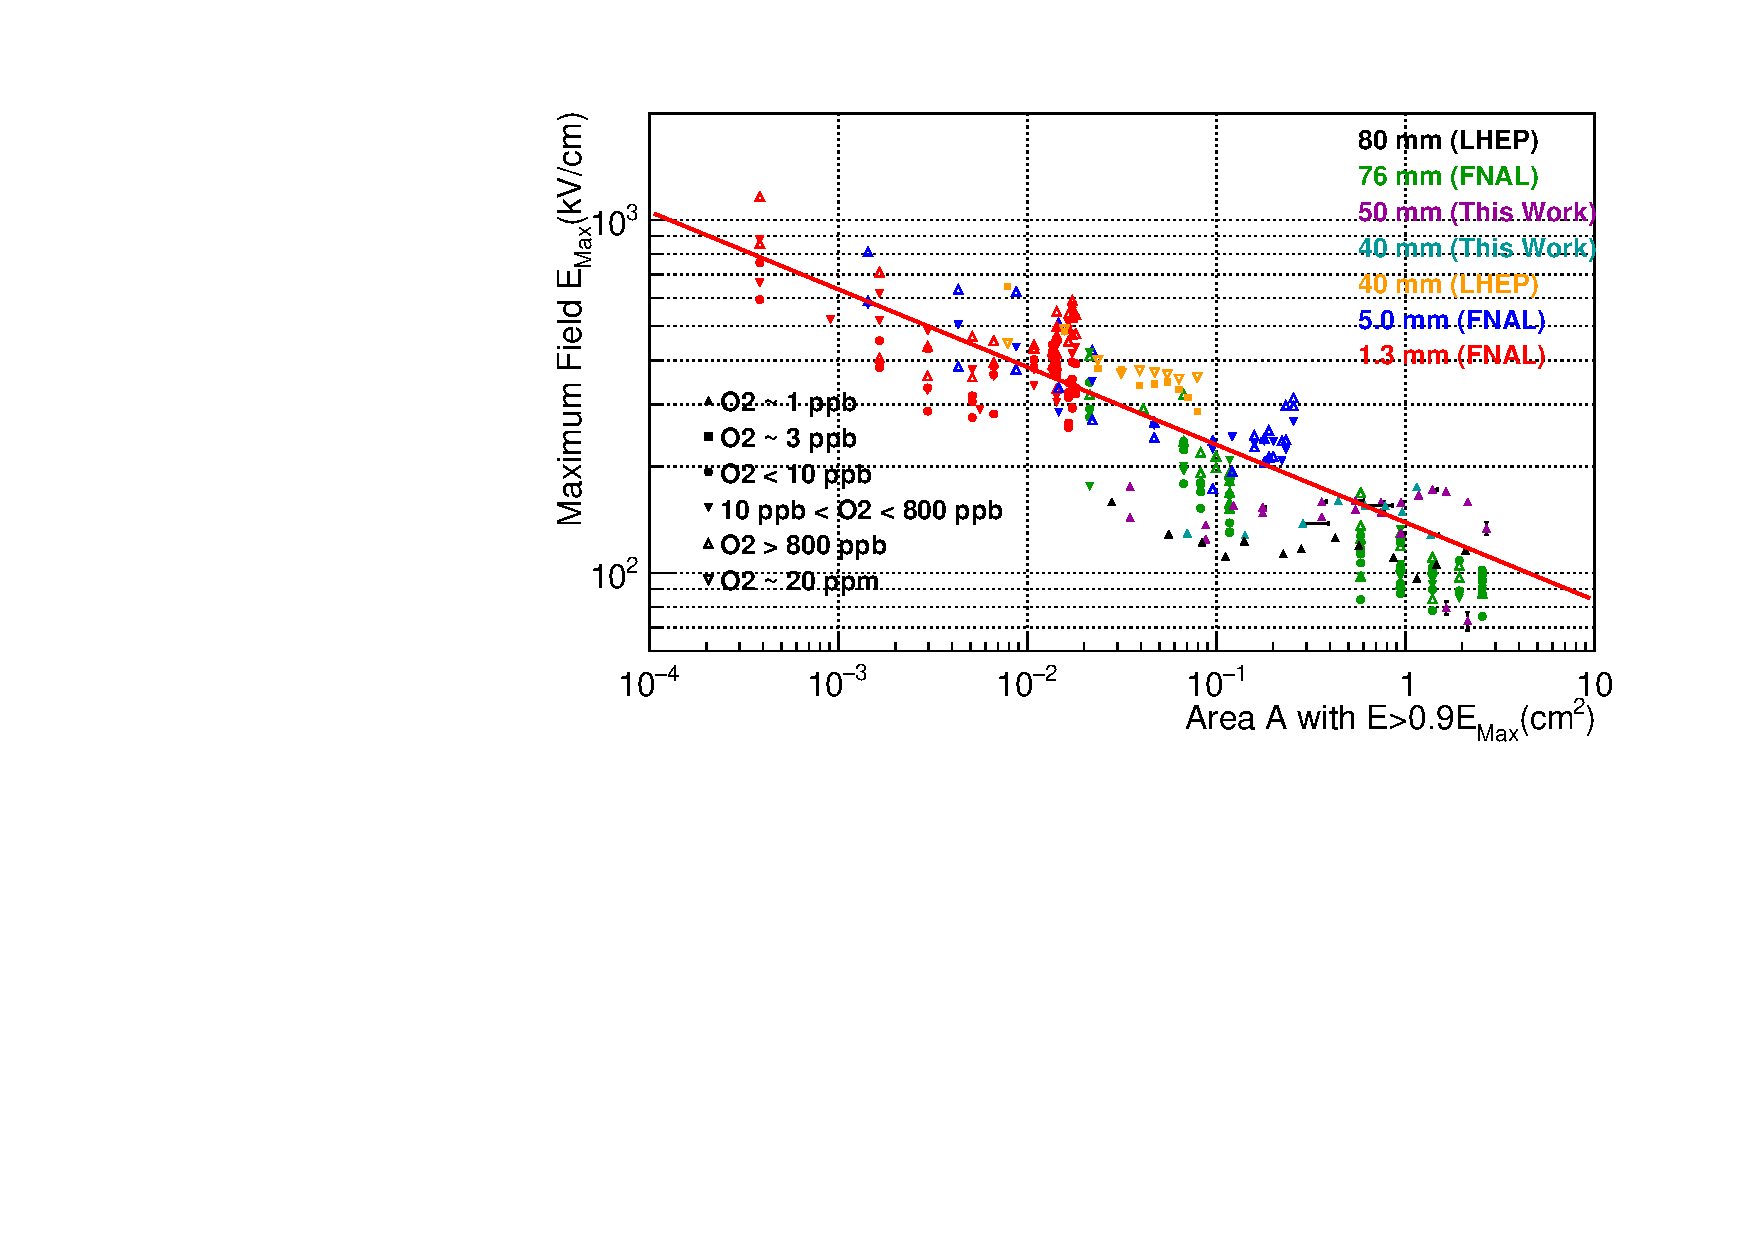
\includegraphics[width=\textwidth]{hv/Area90-1}
	\caption{Breakdown field versus stressed area of the cathode. The stressed area $A$ is defined as the area with an electric field intensity greater than \SI{90}{\percent} of the maximum electric field intensity in the gap. The fit line represents the dependence $E_{max}=C\cdot A^p$ with $C = \num{139 +- 5}$ and $p = \num{-0.22 +- 0.01}$. The colours correspond to different cathode sphere diameters while the marker styles correspond to different oxygen-equivalent impurity concentrations. The data are taken from \cite{FNAL-hv-paper}~(FNAL), \cite{breakdown_14}~(LHEP), and \cite{breakdown_16}~(this work).}
	\label{fig:hv_powerplot}
\end{figure}


Figure~\ref{fig:hv_spectro} shows the recorded spectra of a typical event.
The spectra are integrated over \SI{1}{\milli\second} and approximately correspond to frames \num{3} (blue) and \num{8} (red) in Figure~\ref{fig:hv_images}.
From the observation of the spectra of the emitted light and the discharge appearance, one can distinguish three phases of the breakdown development.
The first phase starts with the field emission of electrons from a point of the cathode metal surface.
The emitted electrons drift to the anode, ionizing and exciting argon atoms.
Frames \num{2} and \num{3} of Figure \ref{fig:hv_images}, the broad current peak of the current in Figure~\ref{fig:hv_iv}, and the blue curve in Figure~\ref{fig:hv_spectro} show the development of the emission.
Evidence for the presence of ionization comes from the analysis of the emission spectrum in the cone formed by drifting electrons.

\begin{figure}[htb]
	\centering
	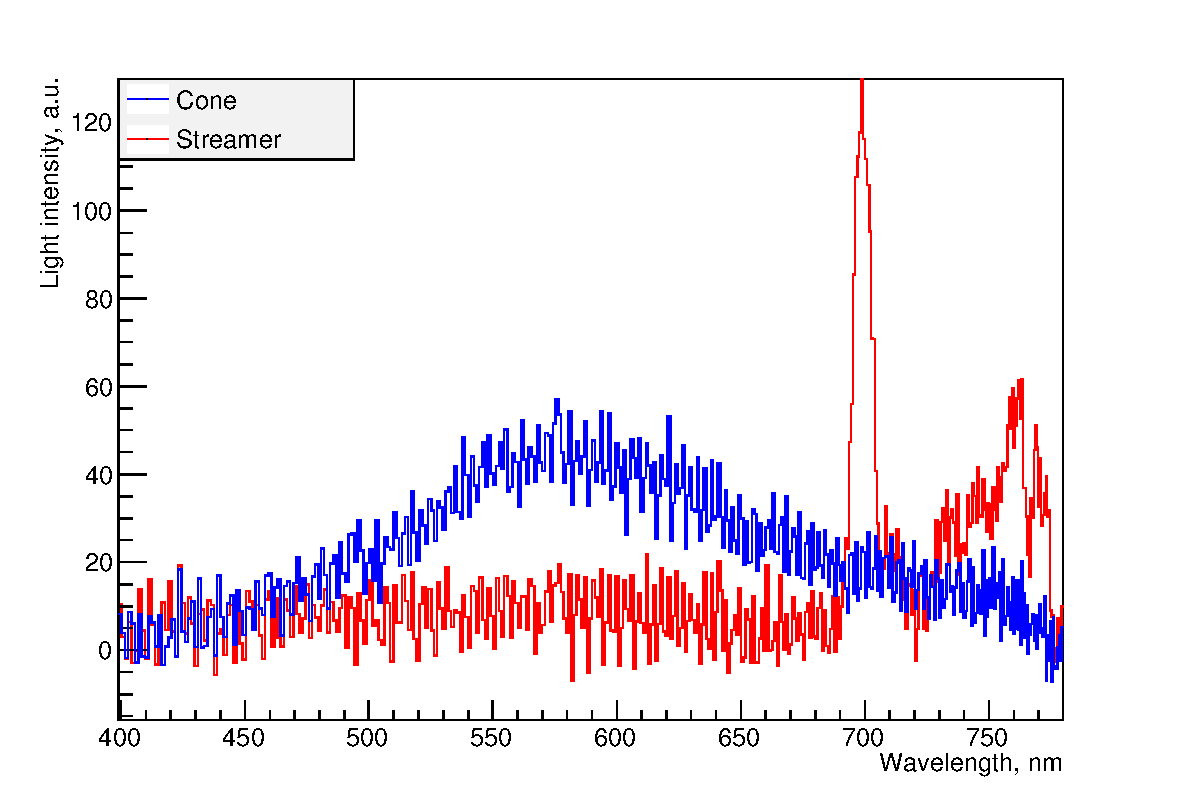
\includegraphics[width=\textwidth]{hv/spectro}
	\caption{Spectra of the field emission cone (blue) and the streamer (red) for a breakdown from a \SI{4}{\centi\metre} diameter cathode at \SI{-56.2}{\kilo\volt} and \SI{3.0}{\milli\metre} apart from the anode plate. The spectra were integrated over a time of \SI{1}{\milli\second} with the spectrum of the streamer taken \SI{2}{\milli\second} after the spectrum of the cone. The blue curve is a broad continuum similar to the scintillation spectrum of liquid argon, while the red curve features a distinct peak around \SI{700}{\nano\metre} which is attributed the the 3p$^5$4p--3p$^5$4s transition of neutral argon gas.}
	\label{fig:hv_spectro}
\end{figure}

The emission of light by charged particles drifting in noble liquids under the influence of an electric field (electro-luminescence) gained great interest in the last years.
Recent studies in this field are well covered by~\cite{buzulutskov1, buzulutskov2, buzulutskov3} and references therein.
The red electro-luminescence, namely the peak around \SI{700}{\nano\metre} of the red curve in Figure~\ref{fig:hv_spectro}, produced by electrons drifting in argon gas is attributed to the 3p$^5$4p--3p$^5$4s transition of neutral argon~\cite{Boffard}.
The energy needed for the excitation of the electrons to the 3p$^5$4p states from the ground state in argon gas is \SIrange{12.9}{13.5}{\electronvolt}.
The ionization potential of liquid argon is \SI{13.84}{\electronvolt}~\cite{2photonAbs}.
For the condensed state, only the scintillation spectrum under ionization by high-energy charged particles has been described in literature so far~\cite{Heindl}.
The electro-luminescence spectrum measured (blue curve in Figure~\ref{fig:hv_spectro}) exhibits a broad continuum, similar to the scintillation spectrum.
However, the center value at about \SI{580}{\nano\metre} does not correspond to any of the electron transitions of neutral, singly- or doubly-ionized argon atoms.
The nearest candidate for such an emission is the residual oxygen with its strong \SI{557.7}{\nano\metre} emission line.
However, if attributable to oxygen, this line has to also be observed at the later stages of the discharge, which does not take place in the measurements.

The broad width of the spectrum could be explained by smearing the energy levels into bands due to inter-atomic interactions in liquid and by the formation of exciton clusters~\cite{Bernstorff, Foerstel}.
If the energy band structure of excitons in liquid argon is continuous, as suggested by the scintillation spectrum, there might be a significant overlap of the band corresponding to the 3p$^5$4p atomic levels and the conduction band above \SI{13.84}{\electronvolt}.
The presence of an observable emission at about \SI{580}{\nano\metre}, in this case, is inevitably linked to a presence of ionized states.

Another signature of avalanche ionization in this phase of the breakdown is the increase of the cone brightness as it develops from the cathode towards the anode.
Figure~\ref{fig:hv_conexpo} shows this increase together with the fit avalanche multiplication parameter $\alpha = \SI{0.15 +- 0.03}{\per\milli\metre}$ for the following gap conditions: voltage across the \SI{7.0}{\milli\metre} gap $V = \SI{54.0}{\kilo\volt}$, cathode sphere diameter of \SI{4}{\centi\metre}, maximum field in the gap $E_{\m{max}} = \SI{96.1}{\kilo\volt\per\centi\metre}$, mean field in the gap $<E> = \SI{87.0}{\kilo\volt\per\centi\metre}$.
To calculate the emission intensity the raw values of all pixels of the camera image were summed up that were in a row perpendicular to the cone direction.
The distance from the cathode can be derived from the known gap distance.
From the fit, the given statistical uncertainty of $\alpha$ was obtained.
As only one measurement was taken, it is not possible to state anything about unknown systematic uncertainties (for instance the calibration of the camera).

\begin{figure}[htb]
	\centering
	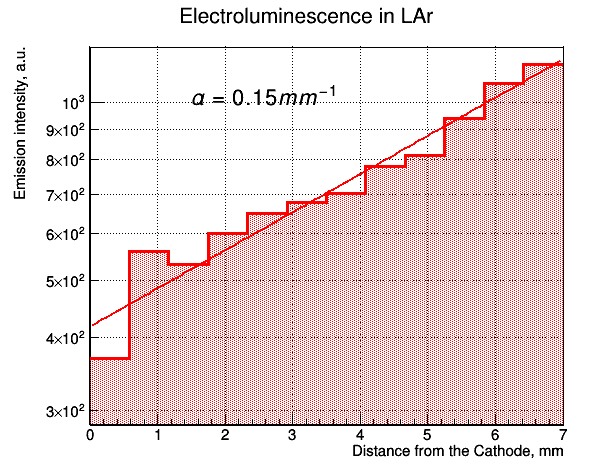
\includegraphics[width=\textwidth]{hv/ConeExpo.png}
	\caption{Increasing brightness of the electro-luminescence cone as it develops towards the anode. The line represents the exponent with a fit avalanche multiplication parameter of $\alpha = \SI{0.15 +- 0.03}{\per\milli\metre}$ for gap conditions: voltage across the \SI{7.0}{\milli\metre} gap $V = \SI{54.0}{\kilo\volt}$, cathode sphere diameter of \SI{4}{\centi\metre}, maximum field in the gap $E_{\m{max}} = \SI{96.1}{\kilo\volt\per\centi\metre}$, mean field in the gap $<E> = \SI{87.0}{\kilo\volt\per\centi\metre}$.}
	\label{fig:hv_conexpo}
\end{figure}

As already suggested in~\cite{breakdown_14}, positive ions produced in this process drift towards the cathode, raising the surface field and provoking a rapid increase of the field emission current to values of the order of several \si{\milli\ampere}.
Ions bombarding the cathode surface raise the local temperature and, after \SIrange{1}{2}{\milli\second}, the liquid near the initial discharge point transitions to a gas phase, forming a bubble.
Both the first and the second avalanche multiplication coefficients are a few orders of magnitude higher in gas than in liquid.
Therefore, the ionization density in the gas bubble quickly rises along with the conductivity of the formed plasma.
This leads to a decrease of the electric field in the close vicinity of the field emission point and to the suppression of a further growth of the field emission current.
Accelerated electrons of the gas plasma hit the gas-liquid interface, forcing the bubble to elongate and grow.
In the region behind the head of the streamer the filament is collapsed to a diameter below \SI{200}{\micro\metre} (the spatial resolution of the camera) by surface tension and electro-striction forces.
This second phase of the discharge is characterized by the growth of the streamer-like filament in liquid.
In Figure~\ref{fig:hv_images} (frames \numrange{4}{10}), one can see the development of such a filament.
Unlike the electrons in the first phase the filament does not follow the electrostatic field lines but it rather rambles around their direction, being subject to thermodynamic fluctuations at the tip of the growing streamer where the liquid-gas transition happens.
The spectrum of the light emission from the streamer has a distinct line at about \SI{700}{\nano\metre}, a characteristic feature of the plasma in argon gas.

\begin{figure}[htb]
	\centering
	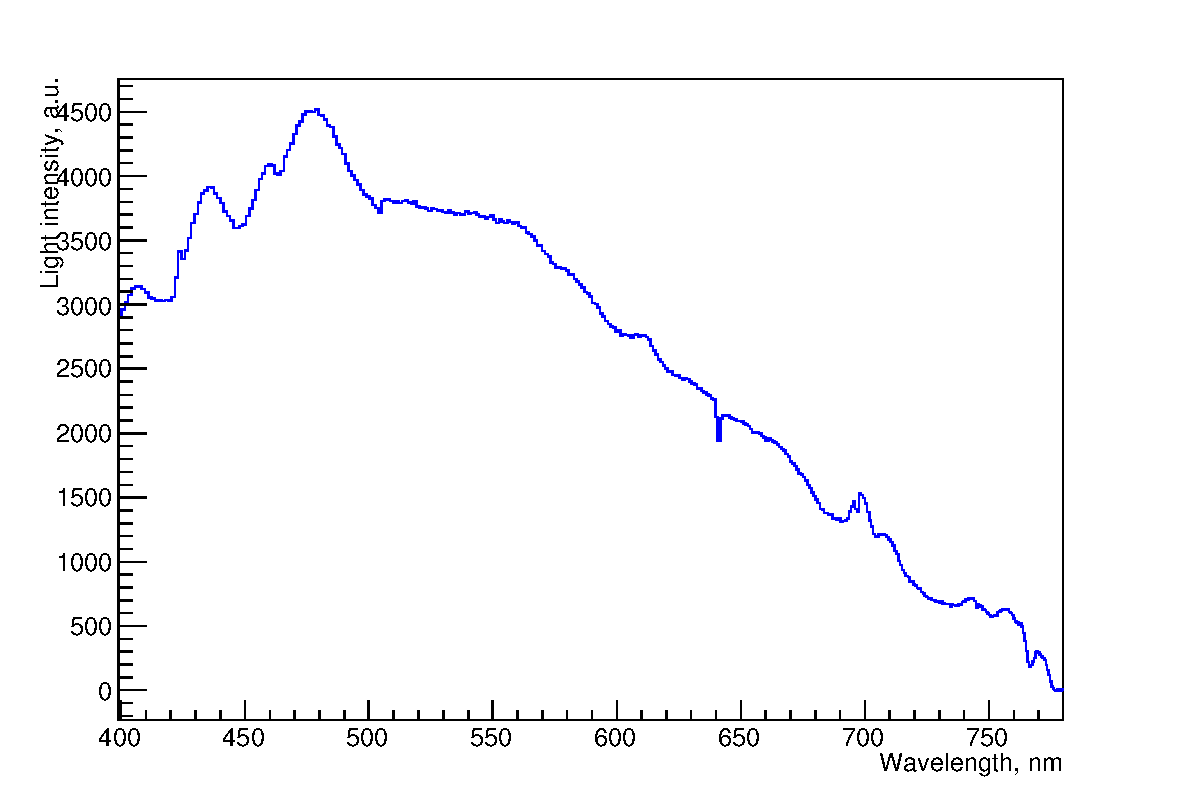
\includegraphics[width=\textwidth]{hv/spectro_spark}
	\caption{Spectrum of the spark for a breakdown from a \SI{4}{\centi\metre} diameter cathode at \SI{-39.7}{\kilo\volt} and \SI{4.0}{\milli\metre} apart from the anode plate. The spectrum was integrated over a time of \SI{1}{\milli\second}.}
	\label{fig:hv_spectro_spark}
\end{figure}

Finally, when the streamer reaches the anode a short peak of light emission is registered (frame \num{11} in Figure~\ref{fig:hv_images}) with the blue-green spectral component dominating (Figure~\ref{fig:hv_spectro_spark}).
This phase is characterized by an acoustic shock and a massive production of gas bubbles in the region of the discharge.
These effects are typical for an arc discharge in argon gas.
The spectrum of the light emission in this phase  is shown in Figure~\ref{fig:hv_spectro_spark}. 

As it was demonstrated in~\cite{Heindl}, the transition from the liquid phase to the gas phase for scintillation manifests itself by the appearance of sharp spectral lines while in liquid, the emission spectrum is continuous and without features.
This behaviour is also suggested by the two spectra in Figure~\ref{fig:hv_spectro}.
While the spectrum is continuous during the field emission phase, there is a distinct peak at around \SI{700}{\nano\metre} several \si{\milli\second} later.

It is worth mentioning that not every streamer results in a third phase spark.
For those streamers started from the side of the cathode sphere, the charge needed for streamer growth might exceed the total charge available in the system.
Such streamers extinguish before reaching the anode without an acoustic shock or any other additional effects.
On the other hand, in some cases the filament quickly transits to a third stage before it reaches the anode.
One possible explanation for this is that, if the filament current exceeds a given threshold, the filament loses its thermodynamic stability and expands into a gas bubble in which the arc discharge quickly develops afterwards.

\begin{figure}[p]
	\centering
	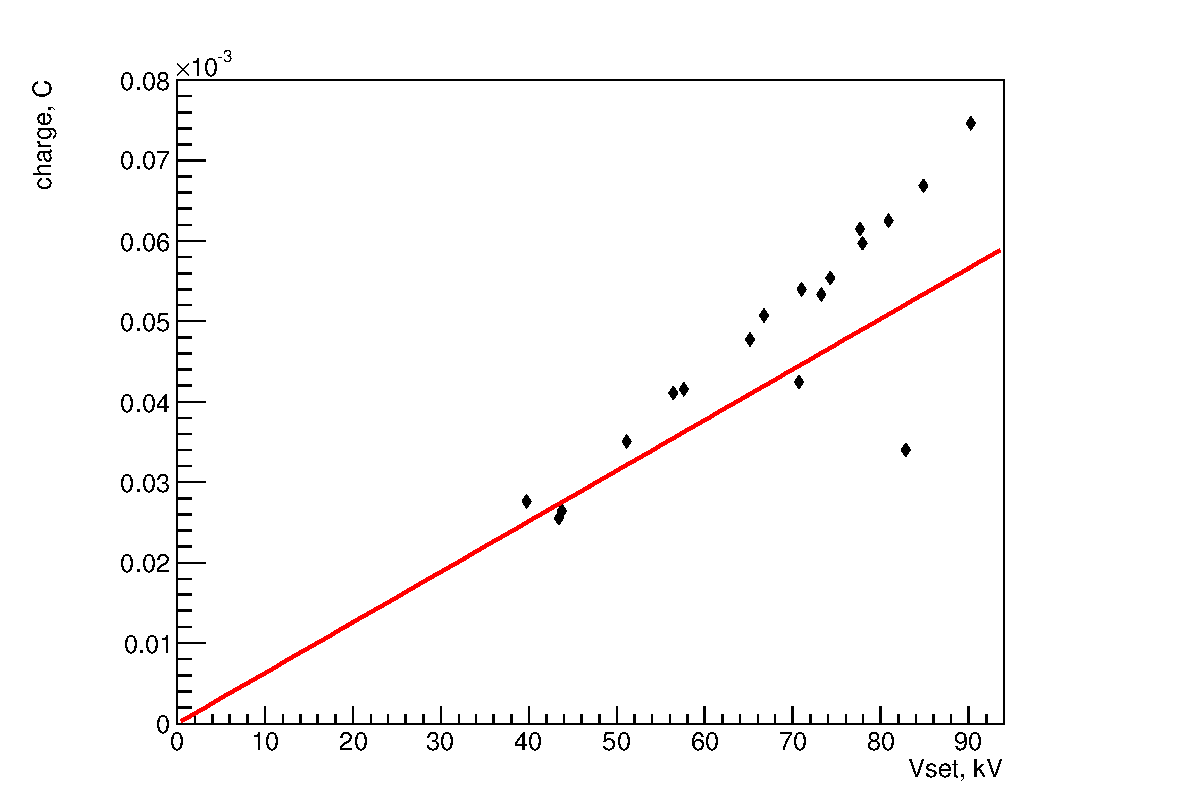
\includegraphics[height=0.43\textheight]{hv/selected_chargeVsVset}
	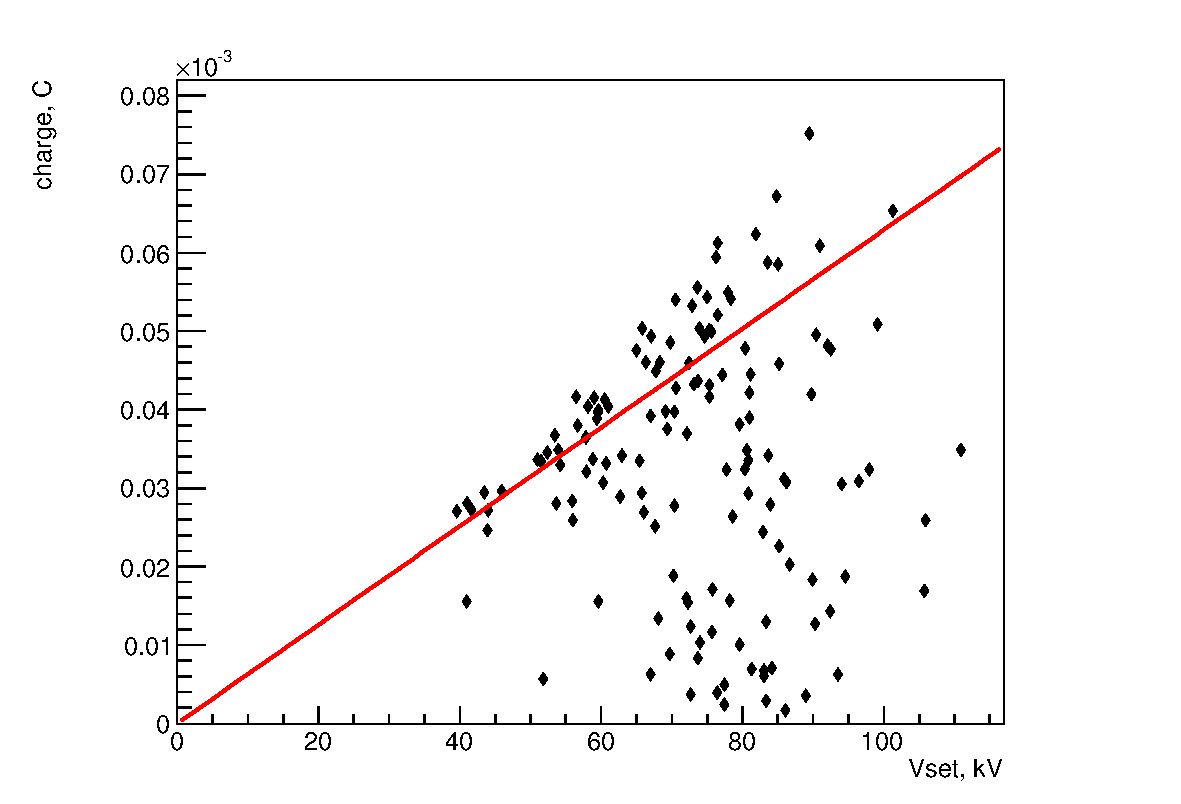
\includegraphics[height=0.43\textheight]{hv/allGood_chargeVsVset}
	\caption{Correlations between integrated charge and breakdown voltage \emph{Vset} for the selected events with distinguishable slow streamer phase (top) and for all events with recorded current characteristics (bottom). The red line represents the charge stored in the gap capacitance using the tuned value of the latter.}
	\label{fig:hv_chargeVsVset}
\end{figure}

\begin{figure}[p]
	\centering
	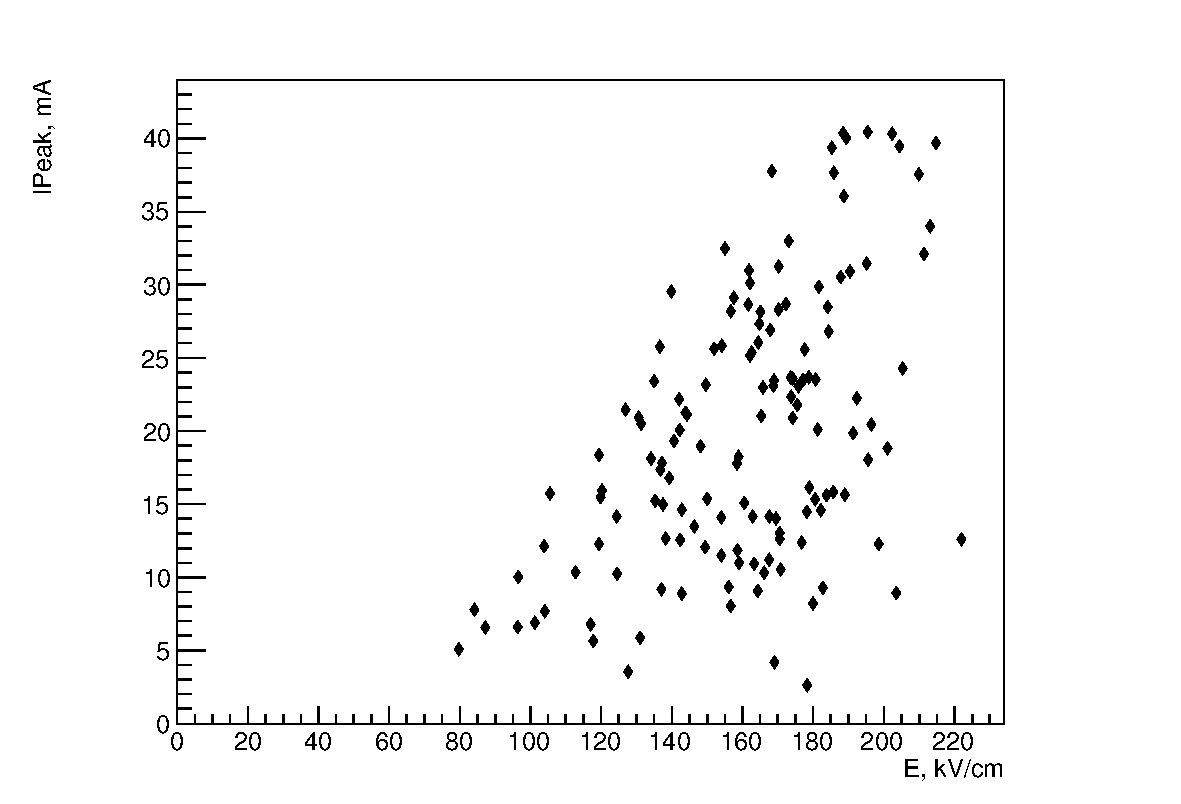
\includegraphics[height=0.4\textheight]{hv/allGood_IPeakVsE}
	\caption{Correlations between peak current \emph{IPeak} and maximum breakdown field \emph{E} for all events with recorded current characteristics.}
	\label{fig:hv_IPeakVsE}
\end{figure}

\begin{figure}[p]
	\centering
	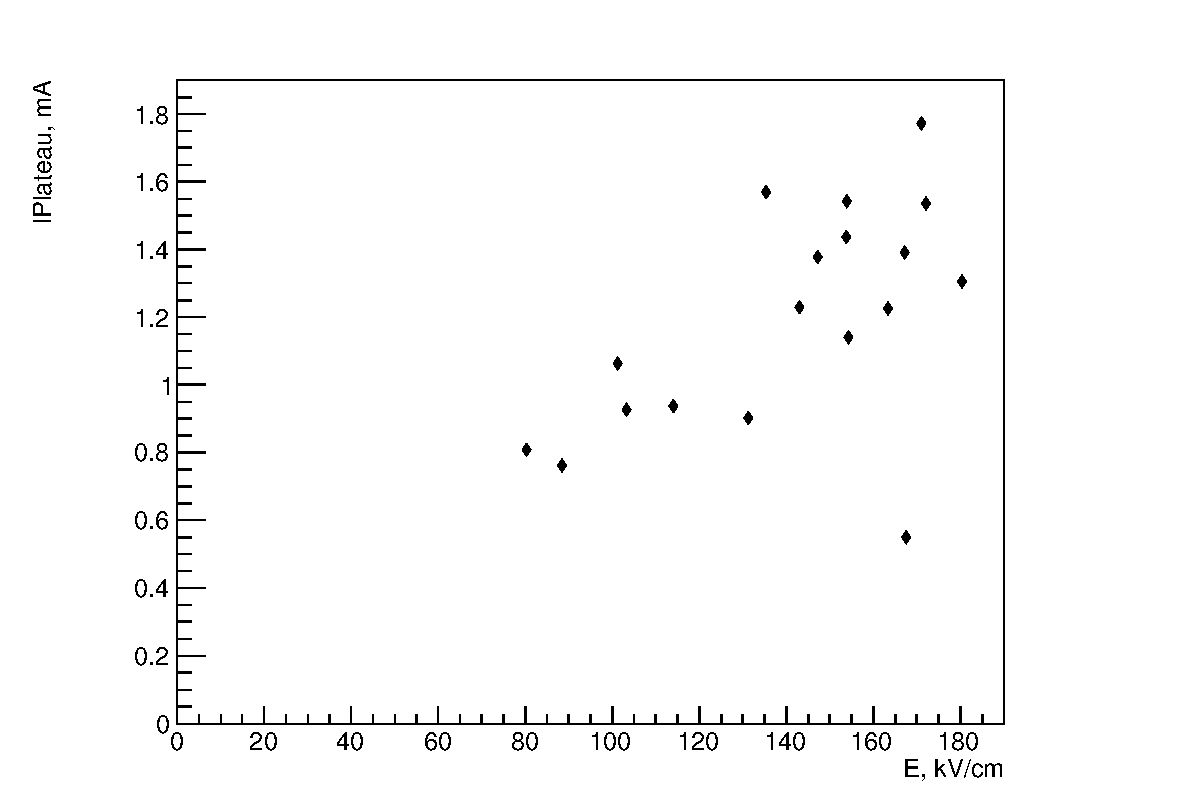
\includegraphics[height=.4\textheight]{hv/selected_IPlateauVsE}
	\caption{Correlations between plateau current \emph{IPlateau} and maximum breakdown field \emph{E} for the selected events.}
	\label{fig:hv_IPlateauVsE}
\end{figure}

\begin{figure}[p]
	\centering
	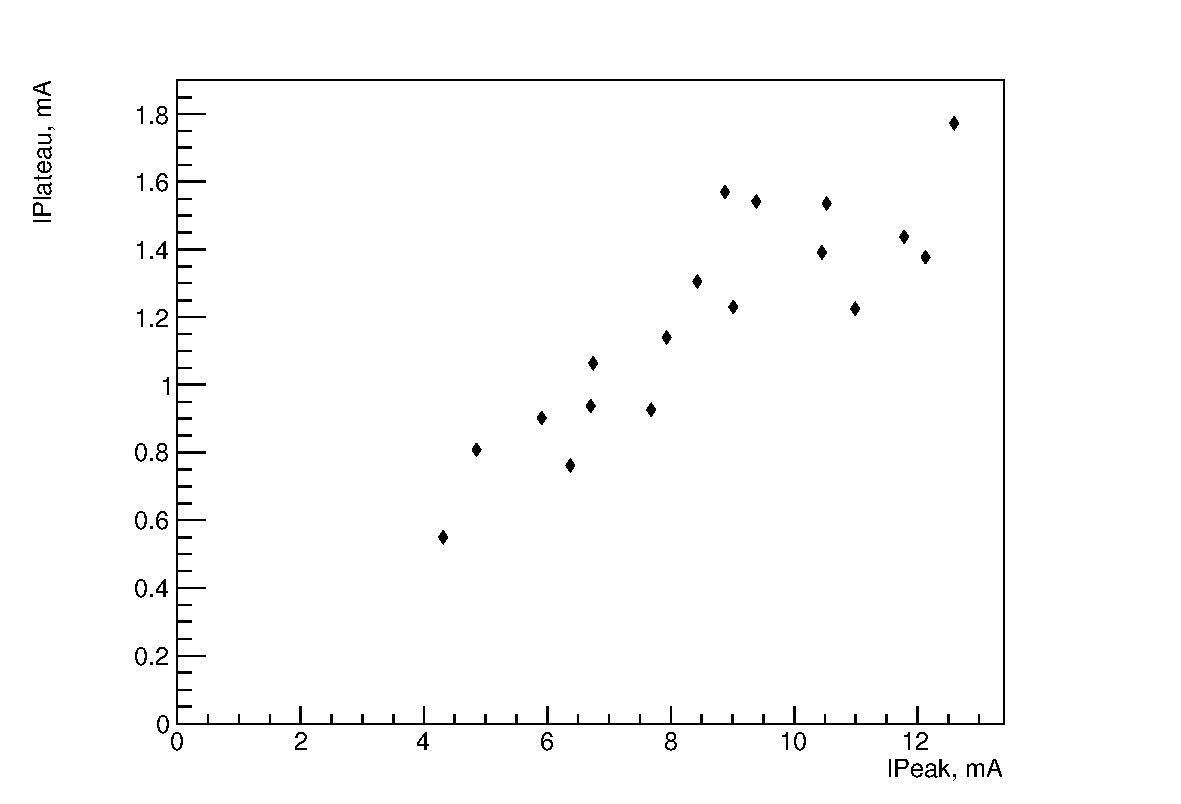
\includegraphics[height=.4\textheight]{hv/selected_IPlateauVsIPeak}
	\caption{Correlations between plateau current \emph{IPlateau} and peak current \emph{IPeak} for the selected events.}
	\label{fig:hv_IPlateauVsIPeak}
\end{figure}

\begin{figure}[p]
	\centering
	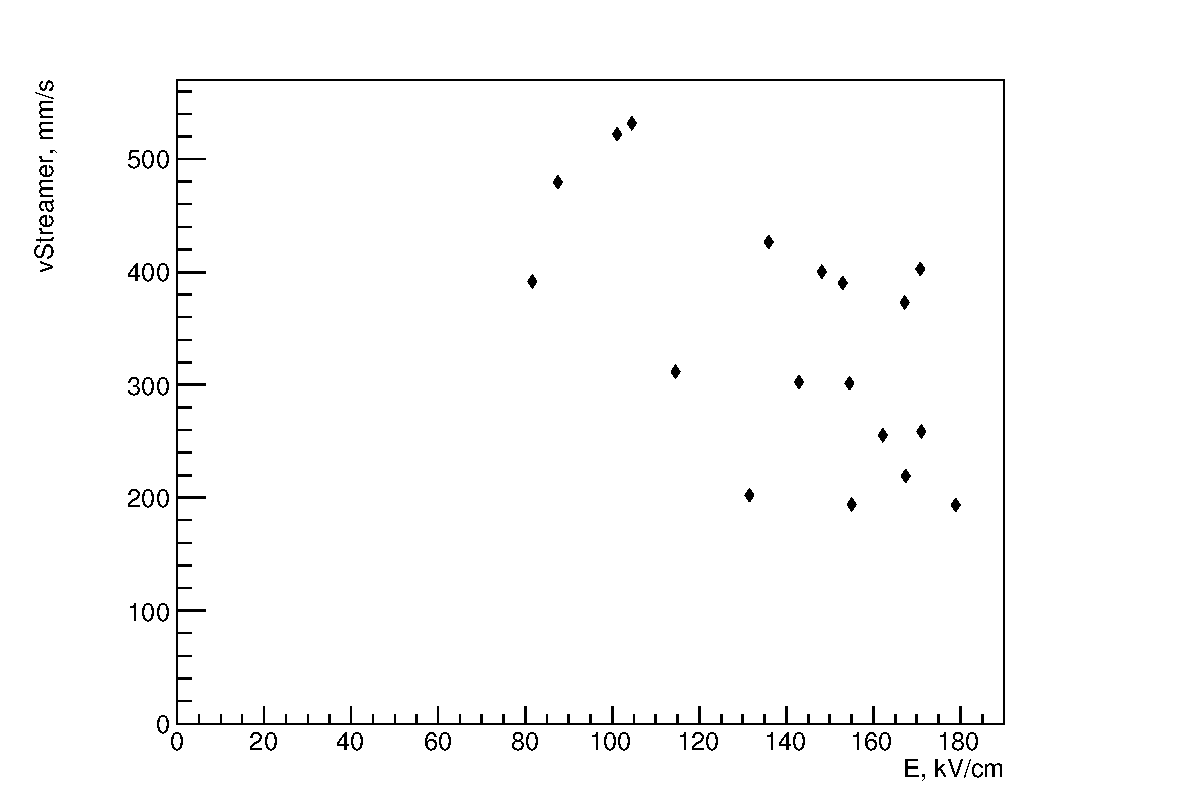
\includegraphics[height=.4\textheight]{hv/selected_vStreamerVsE}
	\caption{Correlations between minimum streamer velocity \emph{vStreamer} and maximum breakdown field \emph{E} for the selected events with a distinguishable slow streamer phase.}
	\label{fig:hv_vStreamerVsE}
\end{figure}

In Figures~\ref{fig:hv_chargeVsVset} to~\ref{fig:hv_vStreamerVsE}, several correlations of measured and calculated parameters of the breakdowns are shown.
For some of these plots, \num{18} events were selected with recorded current characteristics similar to Figure~\ref{fig:hv_iv}.
As a comparison, the bottom plot of Figure~\ref{fig:hv_chargeVsVset} shows the data of all events with current characteristics including events not possessing a distinct plateau as the one visible in Figure~\ref{fig:hv_iv}.
The discrepancy to the total number of events in Table~\ref{tab:hv_table2} arises, on the one hand, because the shunt resistor was installed only in the last run and, on the other hand, since the latter was damaged after the events shown in the bottom plot of Figure~\ref{fig:hv_chargeVsVset}.
The low number of events in the selection is due to the fact that an automated analysis of the current characteristics can only detect very long streamers.
This also explains the behaviour of the charge in Figure~\ref{fig:hv_chargeVsVset}.
The selected streamers last for several \si{\milli\second}, almost always consume the whole charge in the system and then cease without transitioning to a spark.
The slight excess in charge compared to the charge in the gap capacitance (red line) is likely supplied by the PSU before tripping.
Contrary to this, the bottom plot showing all the events contains many events that do not consume all the stored charge and result in a spark.
The good match between the red curve and the data points serves also as a cross-check of the tuned capacitance.

Figure~\ref{fig:hv_IPeakVsE} shows the behavior of the peak current versus the breakdown field, suggesting a proportionality between the two with the coefficient of about \SI{60}{\micro\ampere\centi\metre\per\kilo\volt}.
The field was calculated by dividing the breakdown voltage by the gap distance.
Therefore, this is a mean value along shortest path and does not directly apply to the selected events as most of them emerged from the side of the sphere.

Figures~\ref{fig:hv_IPlateauVsE} and~\ref{fig:hv_IPlateauVsIPeak} show the correlation of the current during the streamer phase (the plateau in Figure~\ref{fig:hv_iv}) with the peak current and the breakdown field.
The plateau current clearly rises with both the breakdown field and the peak current.
Together with Figure~\ref{fig:hv_IPeakVsE} this indicates that for higher fields, higher currents flow during both field emission as well as streamer phases.
As mentioned above, the plateau current could only be reliably detected for the selected events which is why these plots are not shown for all events.

Finally, Figure~\ref{fig:hv_vStreamerVsE} depicts the dependence of the streamer velocity on the breakdown field.
Again, the velocity is only a lower limit as it was calculated by dividing the gap distance by the duration of the streamer, which is not correct for streamers emerging from the side of the sphere.
There are two distinct types of events.
While the selected streamers are rather slow (velocity $\approx \SI{300}{\milli\metre\per\second}$, independent of the field), the whole data set contains much faster events with the total time in the ns scale (not shown).
The knowledge of the streamer velocity can be applied in the design of protection circuits for future \lartpc{}s.
If a breakdown condition is detected during the streamer phase, the high voltage can be killed prior to a disruptive spark phase potentially damaging sensitive detector electronics.


\section{A Method to Suppress Electric Breakdowns in Liquid Argon}
\label{sec:hv_latex}

Besides the thorough characterisation of breakdowns in \lar{}, a way was found to suppress them by coating the field cage with latex.
It was possible to increase the voltage by a factor of \num{10} using this technique.
This study has been published in~\cite{latex}.

The setup was the same as the one used to study the breakdowns, described in Section~\ref{sec:hv_setup}.
Additionally, the cathode sphere was coated by a layer of polymer.
In order to effectively suppress electric breakdowns, the coating needs to have a high dielectric strength while at the same time staying elastic at cryogenic temperatures (\SI{87}{\kelvin} for a \lar{} detector).
Furthermore, the excess electron mobility of the coating needs to be significantly lower than the one of liquid argon.
If this is the case, electrons emitted by the cathode via field emission can accumulate inside the coating layer and in turn locally reduce high fields and thus quench the field emission.

Natural polyisoprene (latex rubber) is a polymer that satisfies the above requirements.
Its dielectric strength is reported to be in the range of \SIrange{1}{2}{\mega\volt\per\centi\metre}~\cite{fizikaDielektrikov}, its dielectric constant is \num{2.1} which is close to the \num{1.6} of liquid argon, and its room temperature resistivity is \SI{1e16}{\ohm\centi\metre}.
A polyisoprene layer of several \SI{100}{\micro\metre} can be deposited on the sphere by dipping the latter in purified latex milk.
After drying at room temperature, the coating is leached in deionised water for several hours and finally vulcanised at \SI{70}{\celsius} for one hour.
Leaching is needed to remove all soluble pollutants contained in natural latex while the vulcanisation increases the tear strength of the coating.
Like this, the polyisoprene layer keeps its integrity and does not crack even after multiple fast cool-down and warm-up cycles to \SI{87}{\kelvin} and back to room temperature, respectively.

In the first measurement, a \SI{4}{\centi\metre} cathode sphere coated with \SI{450}{\micro\metre} of polyisoprene was used.
The test was started at cathode anode gap width of \SI{5}{\milli\metre} and the voltage was ramped up from \SIrange{0}{130}{\kilo\volt} at \SI{50}{\volt\per\second}.
After no breakdown could be observed for several hours, the gap width was decreased to \SI{4}{\milli\metre} after ramping down the voltage.
Again, no breakdown occurred for several hours and subsequently, the gap was decreased to \SI{3}{\milli\metre}.
During this third ramp-up, there was a breakdown at \SI{112}{\kilo\volt}.
This corresponds to a maximum electric field intensity across the gap of \SI{412}{\kilo\volt} which is more than one order of magnitude higher than the required field intensity to provoke breakdowns from an uncoated cathode~\cite{breakdown_14, breakdown_16}.
A summary of the results is given in Table~\ref{tab:latex_table1}.

\begin{table}[htb]
	\centering
	\caption{Summary of the breakdown test measurements with \SI{200}{\micro\metre} and \SI{450}{\micro\metre} thick polyisoprene layers coated \SI{5}{\centi\metre} and \SI{4}{\centi\metre} diameter spheric cathodes, respectively.}
	\label{tab:latex_table1}
	\begin{tabu} to \textwidth {|S|S|S|S|l|}
		\hline
		{{$d_{\m{Gap}}$}} &		{{$E_{\m{max}}$}} &						$\varnothing_{\m{Sphere}}$ &	{Polyisoprene thickness} &	{Breakdown} \\
		\hline
		\hline
		\SI{5}{\milli\metre} &	\SI{298}{\kilo\volt\per\centi\metre} &	\SI{4}{\centi\metre} &		\SI{450}{\micro\metre} &	{no} \\
		\hline
		\SI{4}{\milli\metre} &	\SI{358}{\kilo\volt\per\centi\metre} &	\SI{4}{\centi\metre} &		\SI{450}{\micro\metre} &	{no} \\
		\hline
		\SI{3}{\milli\metre} &	\SI{412}{\kilo\volt\per\centi\metre} &	\SI{4}{\centi\metre} &		\SI{450}{\micro\metre} &	{yes} \\
		\hline
		\SI{3}{\milli\metre} &	\SI{296}{\kilo\volt\per\centi\metre} &	\SI{5}{\centi\metre} &		\SI{200}{\micro\metre} &	{yes} \\
		\hline
	\end{tabu}
\end{table}
\chapter{Electronics studies\label{chap:electronics}}
For a heavy MIP $\dv{E}{x} \approx \SI{2}{\mega\electronvolt\per\centi\metre}$, a \lartpc\ has a charge yield of $\order{\SI{1}{\femto\coulomb\per\milli\metre}}$ as explained in Chapter~\ref{chap:lartpc}.
The readout electronics need to be able to reliably digitise this charge.
This chapter aims to outline the challenges based on present designs and then present several tests of future approaches addressing them.


\section{Existing chain\label{sec:electronics_existing}}

Contemporary electronics schemes shall be introduced by looking at the existing readout chain at LHEP at the University of Bern.
It was originally designed for the \AT\ experiment and a more detailed description can be found in~\cite{AT_larasic}.

The charge collected by the readout plane is amplified by LARASIC4*~\cite{larasic} cryogenic charge amplifiers developed by Brookhaven National Laboratory (BNL) for the MicroBooNE experiment~\cite{uboone}.
A performance characterisation of these application-specific integrated circuits (ASICs) can be found in~\cite{AT_larasic}.
Their main features include

\begin{itemize}
	\item \num{16} channels per ASIC;
	\item low noise charge amplifiers incorporating high-order filters;
	\item per channel programmable gain of \SIlist[list-final-separator = { or }]{4.7; 7.8; 14; 25}{\milli\volt\per\femto\coulomb};
	\item per channel programmable filter peaking time of \SIlist[list-final-separator = { or }]{0.5; 1.0; 2.0; 3.0}{\micro\second};
	\item built-in test capacitance connected to dedicated external test pulse input for calibration;
	\item and a power dissipation \SI{< 10}{\milli\watt} per channel.
\end{itemize}

\begin{figure}[htb] %TODO: change ASIC picture
	\centering
	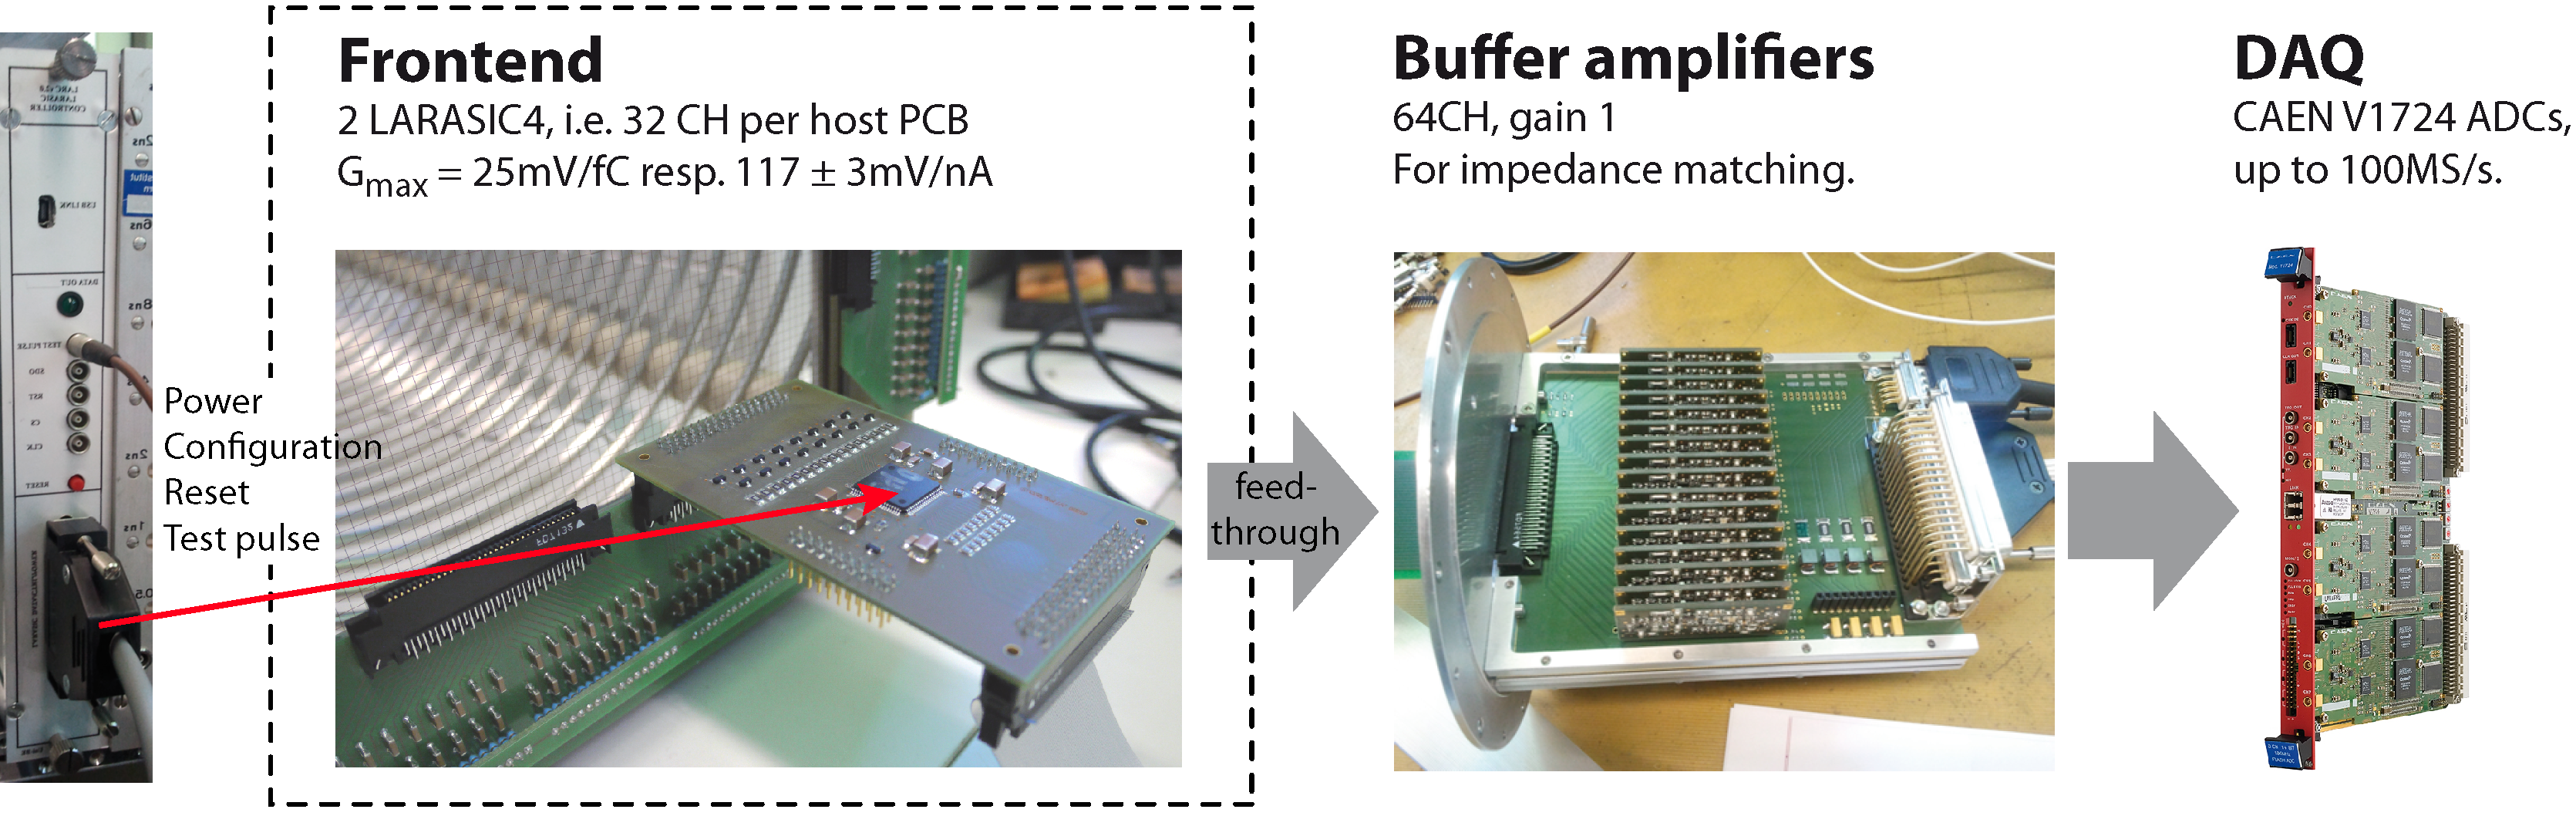
\includegraphics[width=\textwidth]{viper/ReadoutChain_old}
	\caption{Readout chain used for the pixel test. The picture of the LARASIC cryogenic front-end preamplifiers shows them installed in an older wire readout setup.~\cite{AT_larasic}}
	\label{fig:viper_readoutChain_old}
\end{figure}

The cryogenic preamplifiers are mounted as close as possible to the readout in order to minimise noise pick-up on these very sensitive lines.
Via an inter-integrated circuit (I$^2$C) bus, the LARASICs can be programmed to the different aforementioned configurations.
For this purpose, they are connected to a bespoke NIM module housing an Arduino which generates the I$^2$C signals, a test pulse generator, and multiple low-noise voltage regulators providing power to the LARASICs.
By means of flexible Kapton ribbon cables, the output of the preamplifiers is fed to buffer amplifiers mounted on top of the signal feedthrough.
The latter operate at room temperature, have a unity gain, and match the output impedance of the LARASICs to the \SI{50}{\ohm} input impedance of the downstream digitisers.
From the buffers, the signals are routed via \SI{50}{\ohm} unbalanced coaxial lines to \emph{CAEN V1724}\footnote{\href{http://www.caen.it}{http://www.caen.it}} \SI{14}{bit} digitisers sitting in a VME crate.
For debugging purposes, the output of the buffers can be routed to an oscilloscope via a coaxial T-piece.
Finally, the digital data is read out from the VME crate via a fibre-optic link by a standard PC.
Figure~\ref{fig:viper_readoutChain_old} depicts the entire readout chain.
The complete analogue signal path from the pixel plane to the VME digitisers is single-ended and thus prone to ground loops and all the accompanying noise problems.


\section{Tunings after the first measurement campaign\label{sec:electronics_tuning}}

\begin{figure}[htb] %TODO: picture
	\centering
	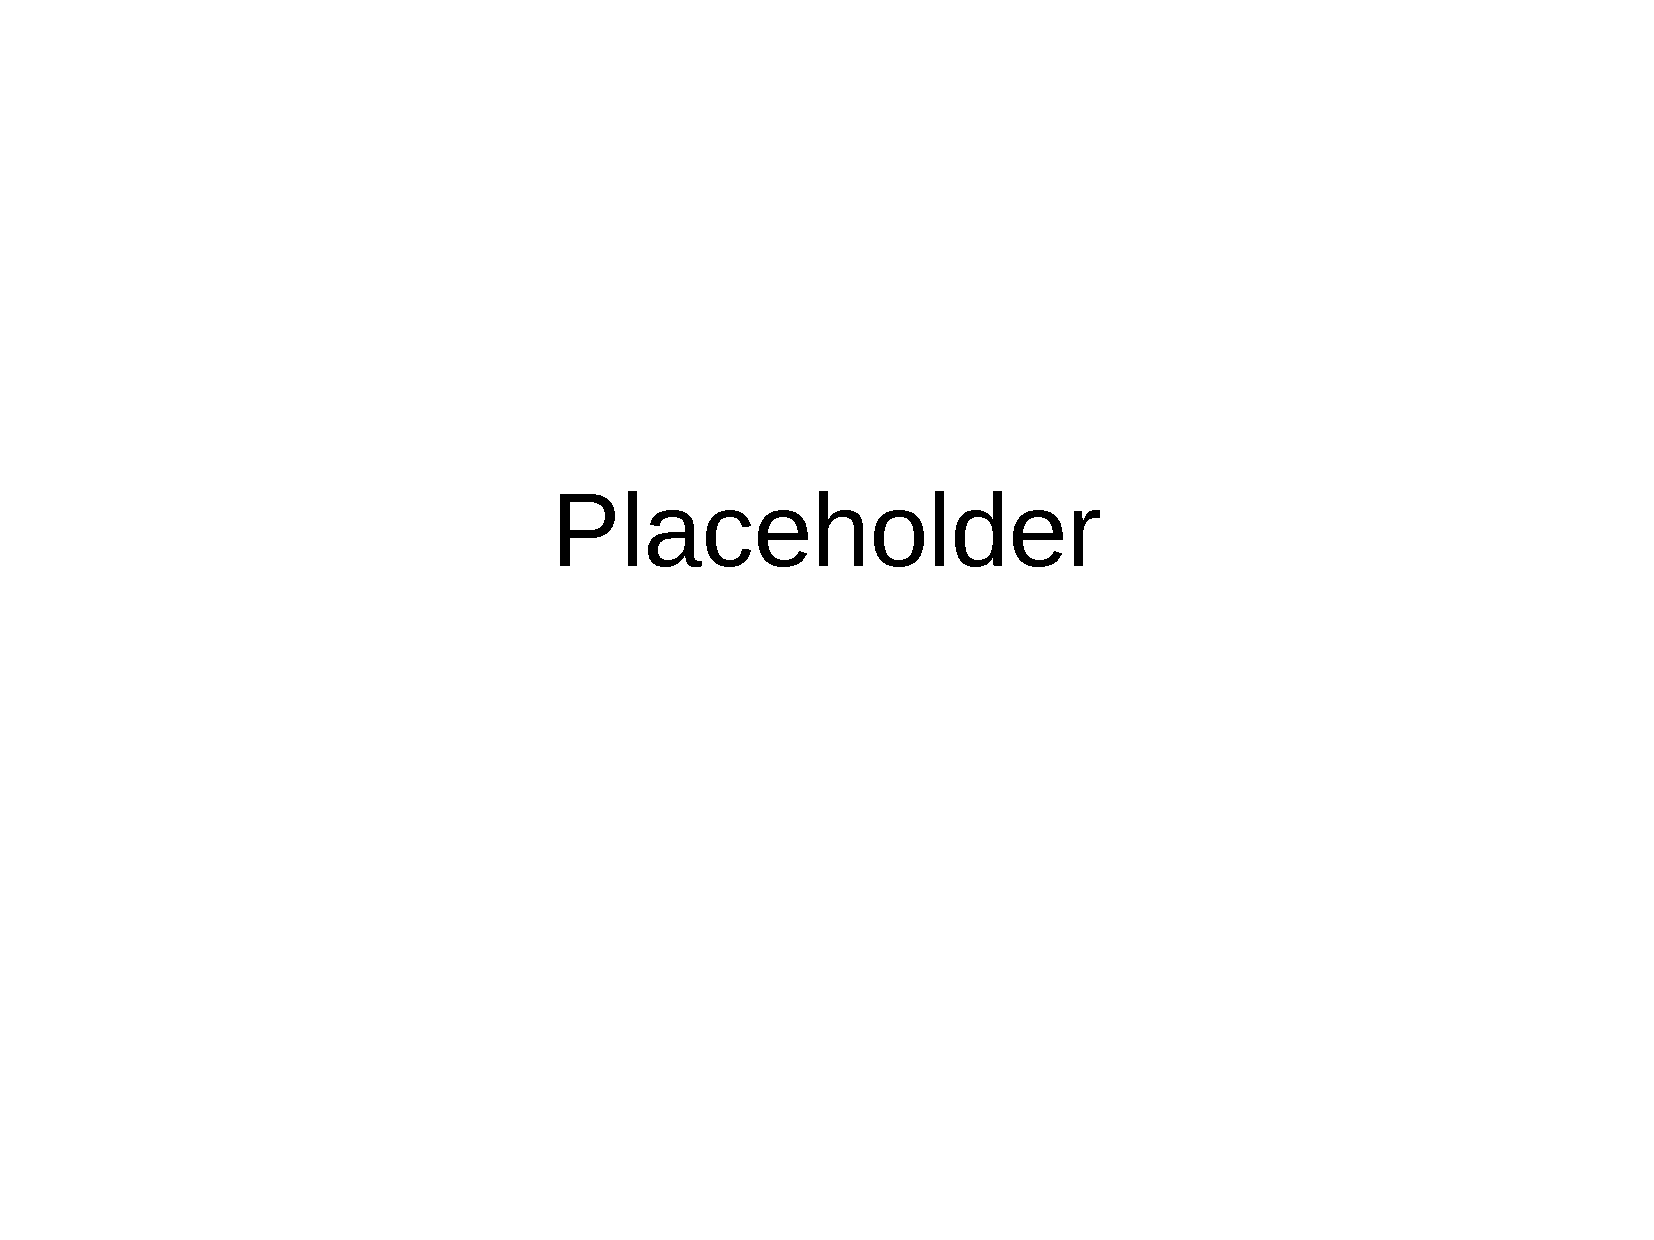
\includegraphics[width=\textwidth]{placeholder}
	\caption{Event from the first measurement campaign of the pixel prototype.}
	\label{fig:viper_noisy-event}
\end{figure}

During the first measurement campaign using a pixelated readout, it became apparent that the data is significantly impaired by noise.
As can be seen in Figure~\ref{fig:viper_noisy-event}, the noise amplitude is similar over multiple channels.
This implies a common mode component that cannot originate from inductive pickup.
Instead, the noise is likely generate by self-oscillating parts of the signal path due to ground loops and parasitic impedances.
For the second measurement campaign, different measures were take to mitigate this behaviour.

The first measure was to build a decoupled clean power grid in the lab.
A motor generator (M-G set) separates the special grid mechanically from the building power supply.
Thus, any noise present on the latter is prevented from entering the experimental setup.
Furthermore, this decouples the special grid entirely from the building ground preventing ground loops via the power supply.

A second measure consisted of changing the signal path from the impedance matching buffer amplifiers to the digitisers---i.e. the warm signal path---from single-ended to differential signalling.
For conventional single-ended signalling, the signal is measured as the voltage or current difference between a signal conductor and a ground common to the signal source and the signal sink.
Using a common ground as signal return path can have several undesired effects.
To shield the signal conductor, it is usually enclosed in a ground shield.
If the latter is connected on both sides, a ground loop can result for instance in combination with a shared power supply ground.
Ground loops can pick up noise through induction if the resistance along the loop is high enough.
A second way to couple noise into a single-ended system is by shifting the potential on the common ground away from the reference voltage or current, for instance due to high currents flowing through a lossy ground connection.
Because the signal is always measured against the common ground, it will be distorted.
In differential signalling, the signal is not measured between a signal conductor and ground but instead between two signal conductors.
This works by putting an inverted waveform of the signal on a second conductor.
The signal is recovered by taking the difference between to two signal conductors.
As a result, the signal sink needs not be connected to the same ground as the signal source because the signal is independent of ground.
Ground loops can thus be avoided in the signal path.
Furthermore, the effects of noise pickup on the signal lines is drastically reduced.
Due to the completely symmetric signal path, inductive noie pickup is equal on both signal conductors as opposed to single-ended signals where the signal path is not symmetric.
In the signal sink, the difference between the two symmetric signal conductors is formed and everything that is present on both of them such as the inductively picked up noise cancels out.
In the pixel prototype setup, differential signalling was realised by replacing the buffer amplifiers by single-ended to differential amplifiers and inserting another stage upstream of the digitisers to change the signal back to \SI{50}{\ohm} single-ended, matching the input of the digitisers.
Like this, noise pick up outside the cryostat could be reduced as well as sensitivity to ground loops between the detector and the DAQ rack.

A third source of noise was identified in the layout of the pixel readout plane.
It was found that due to several ground planes and long tracks in the PCB, parasitic capacitances were very high, in particular for pixel channels.
This is problematic because for high enough frequencies---determined by $RC$---, the input is shorted to ground creating a ground loop again.
Through this capacitive coupling to ground, the system can start to oscillate.
One evidence for this is that the noise is equal over multiple channels, so-called common-mode noise.
More specifically, the noise is equal over groups of channels.
Investigating this, it was found that these groups correspond to channels of roughly equal parasitic capacitance.
Also, the noise amplitude is higher on channels with higher capacitance.
To solve this problem, the PCB design was optimised by removing unnecessary ground planes, routing signal tracks outside necessary ground planes and increasing the thickness of the PCB.

\begin{figure}[htb] %TODO: picture
	\centering
	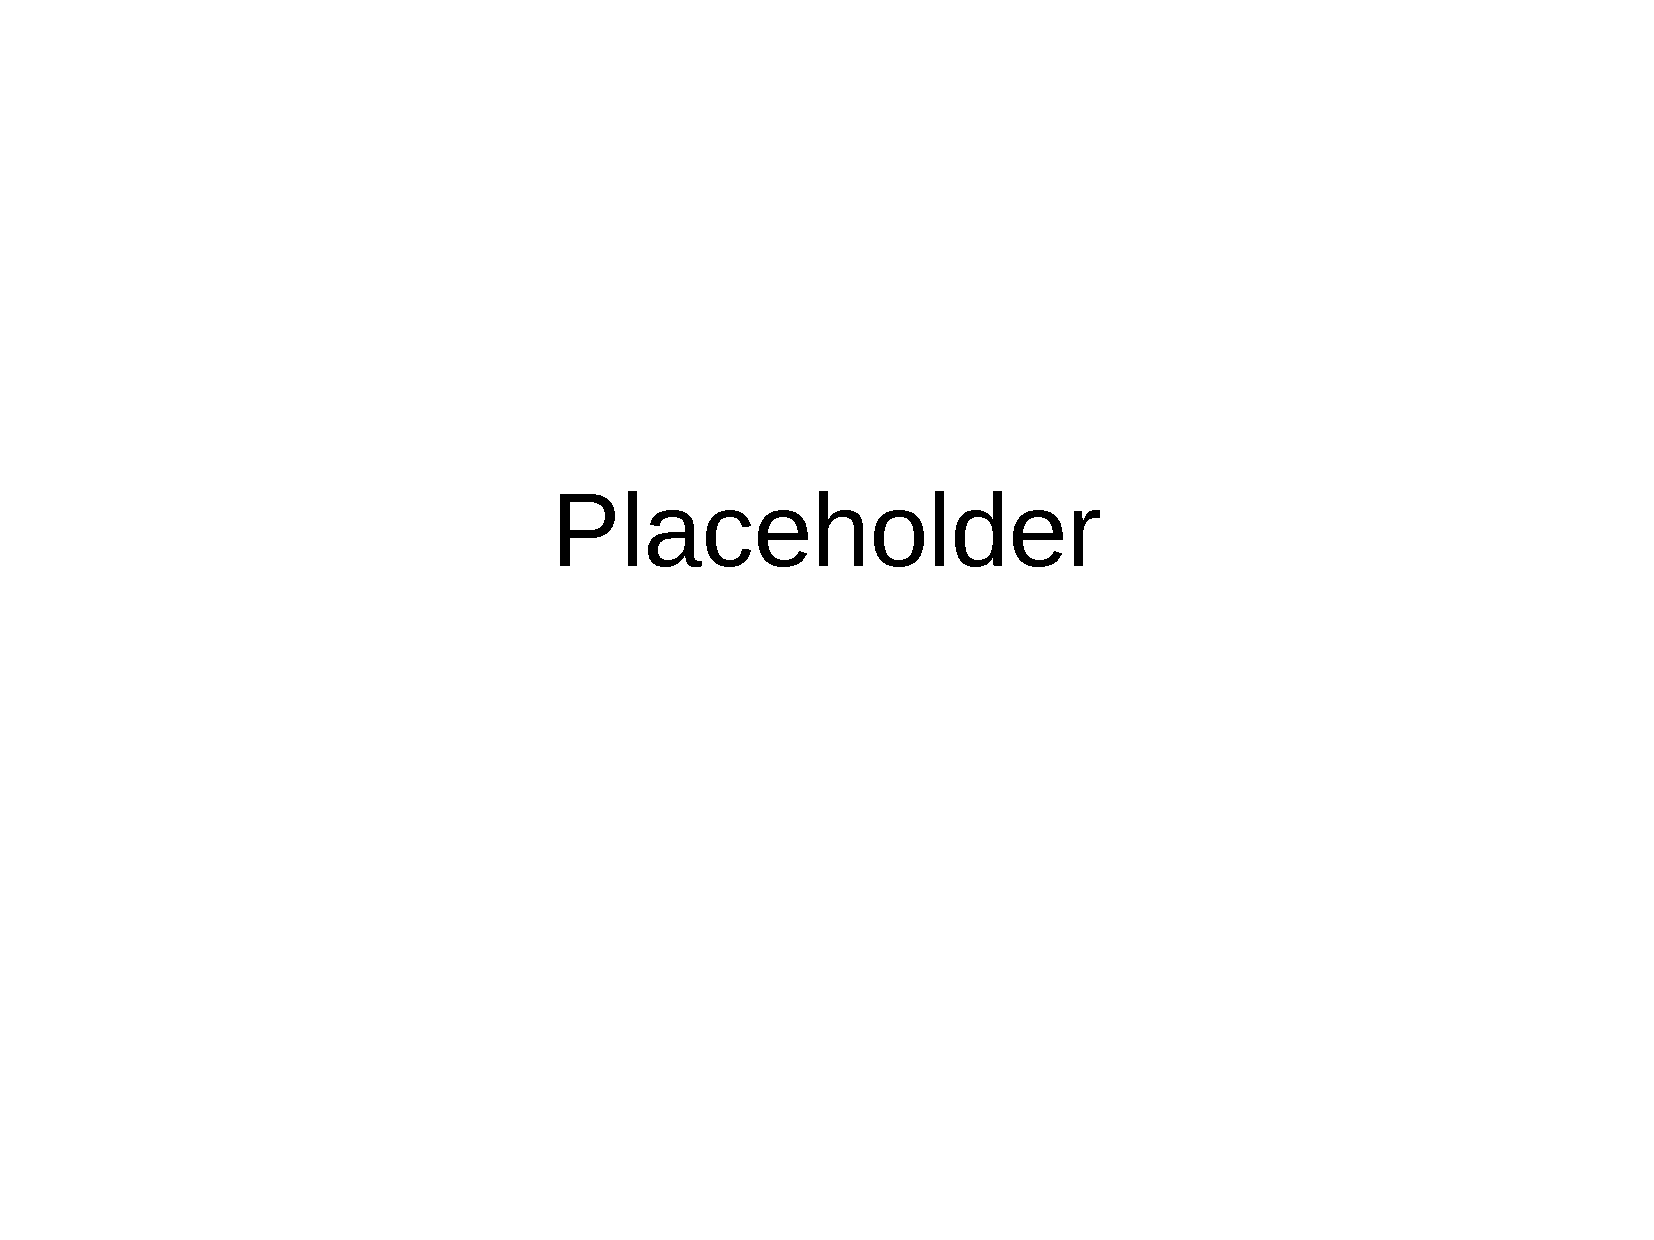
\includegraphics[width=\textwidth]{placeholder}
	\caption{Event from the second measurement campaign of the pixel prototype after improving the readout chain.}
	\label{fig:viper_good-event}
\end{figure}

As can be seen from Figures~\ref{fig:viper_noisy-event} and~\ref{fig:viper_good-event}, there is a significant decrease in noise after commissioning all of the above improvements to the readout chain.
This can also be seen from Figures~\ref{fig:viper_snr-noisy} and~\ref{fig:viper_snr-good} depicting the signal to noise ratio of the two measurement campaigns.

\begin{figure}[htb] %TODO: picture
	\centering
	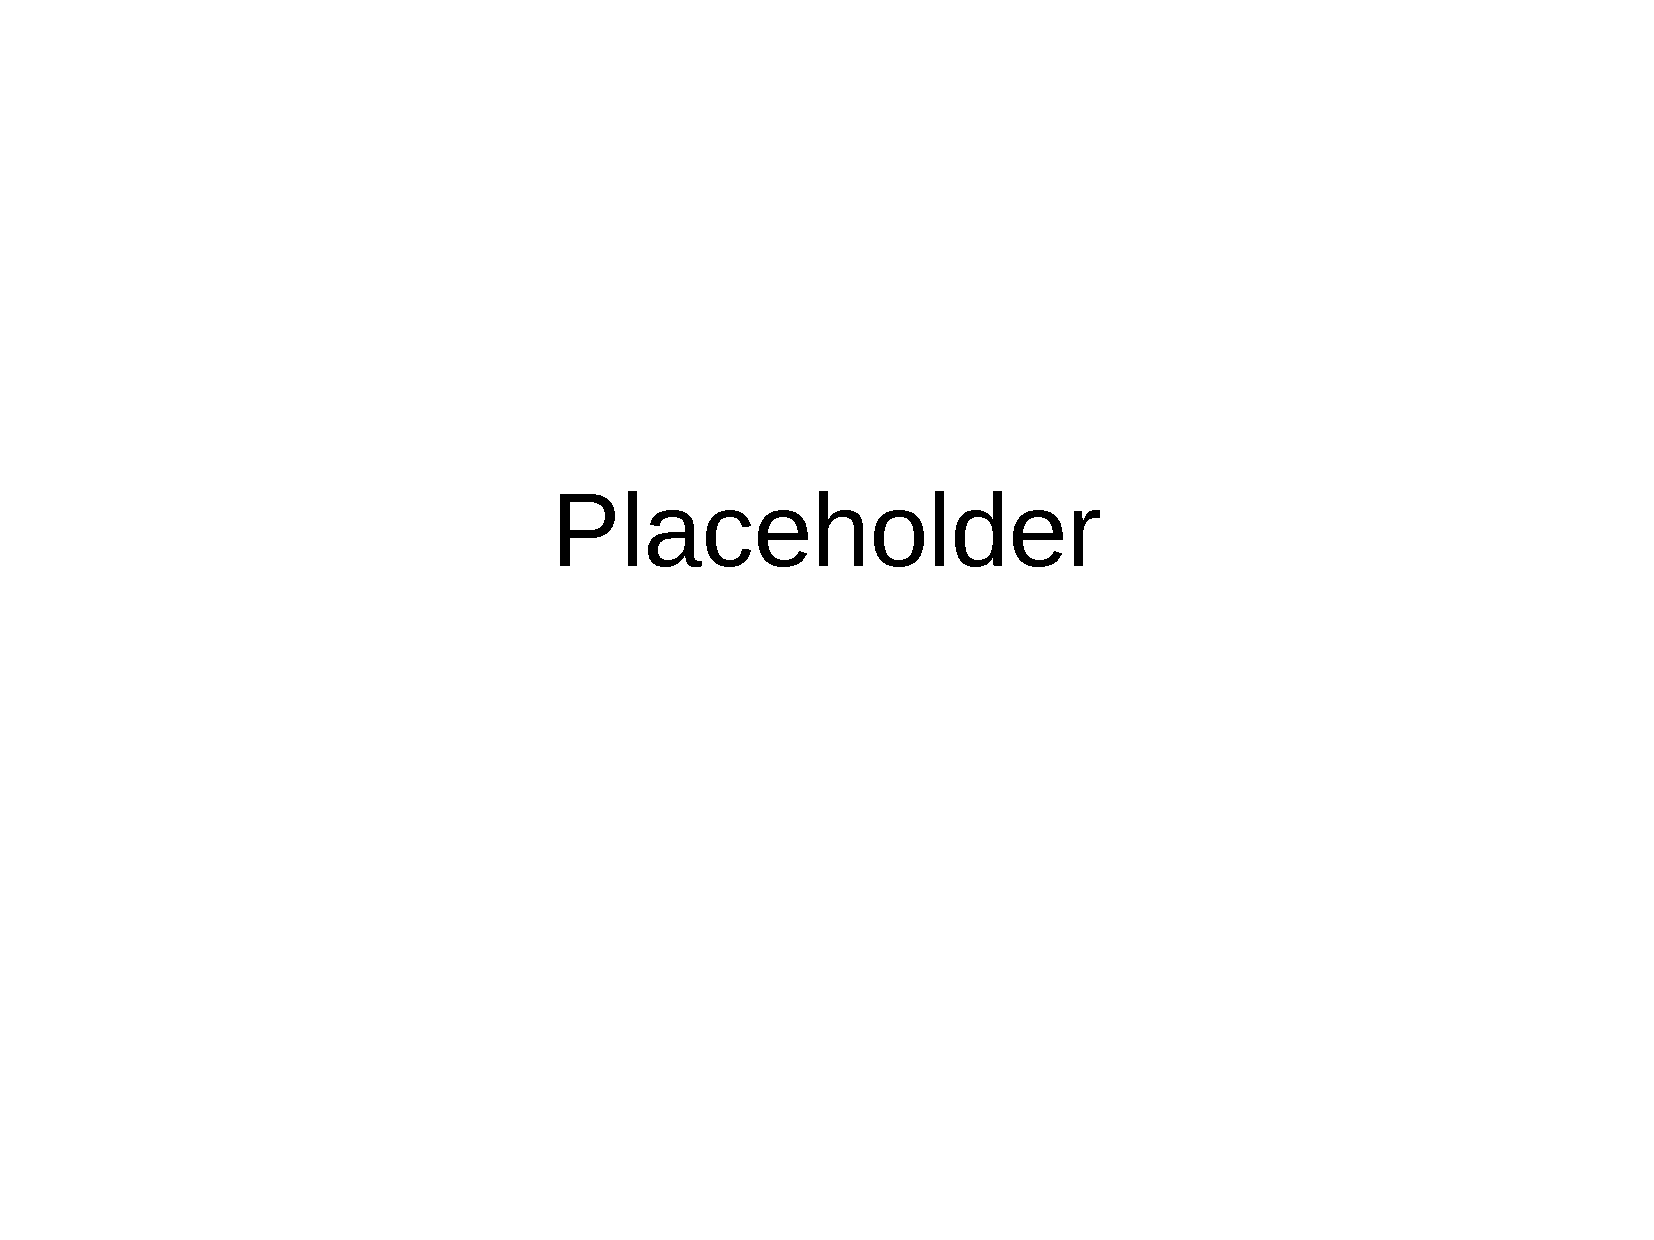
\includegraphics[width=\textwidth]{placeholder}
	\caption{Signal vs noise using the old readout chain.}
	\label{fig:viper_snr-noisy}
\end{figure}

\begin{figure}[htb] %TODO: picture
	\centering
	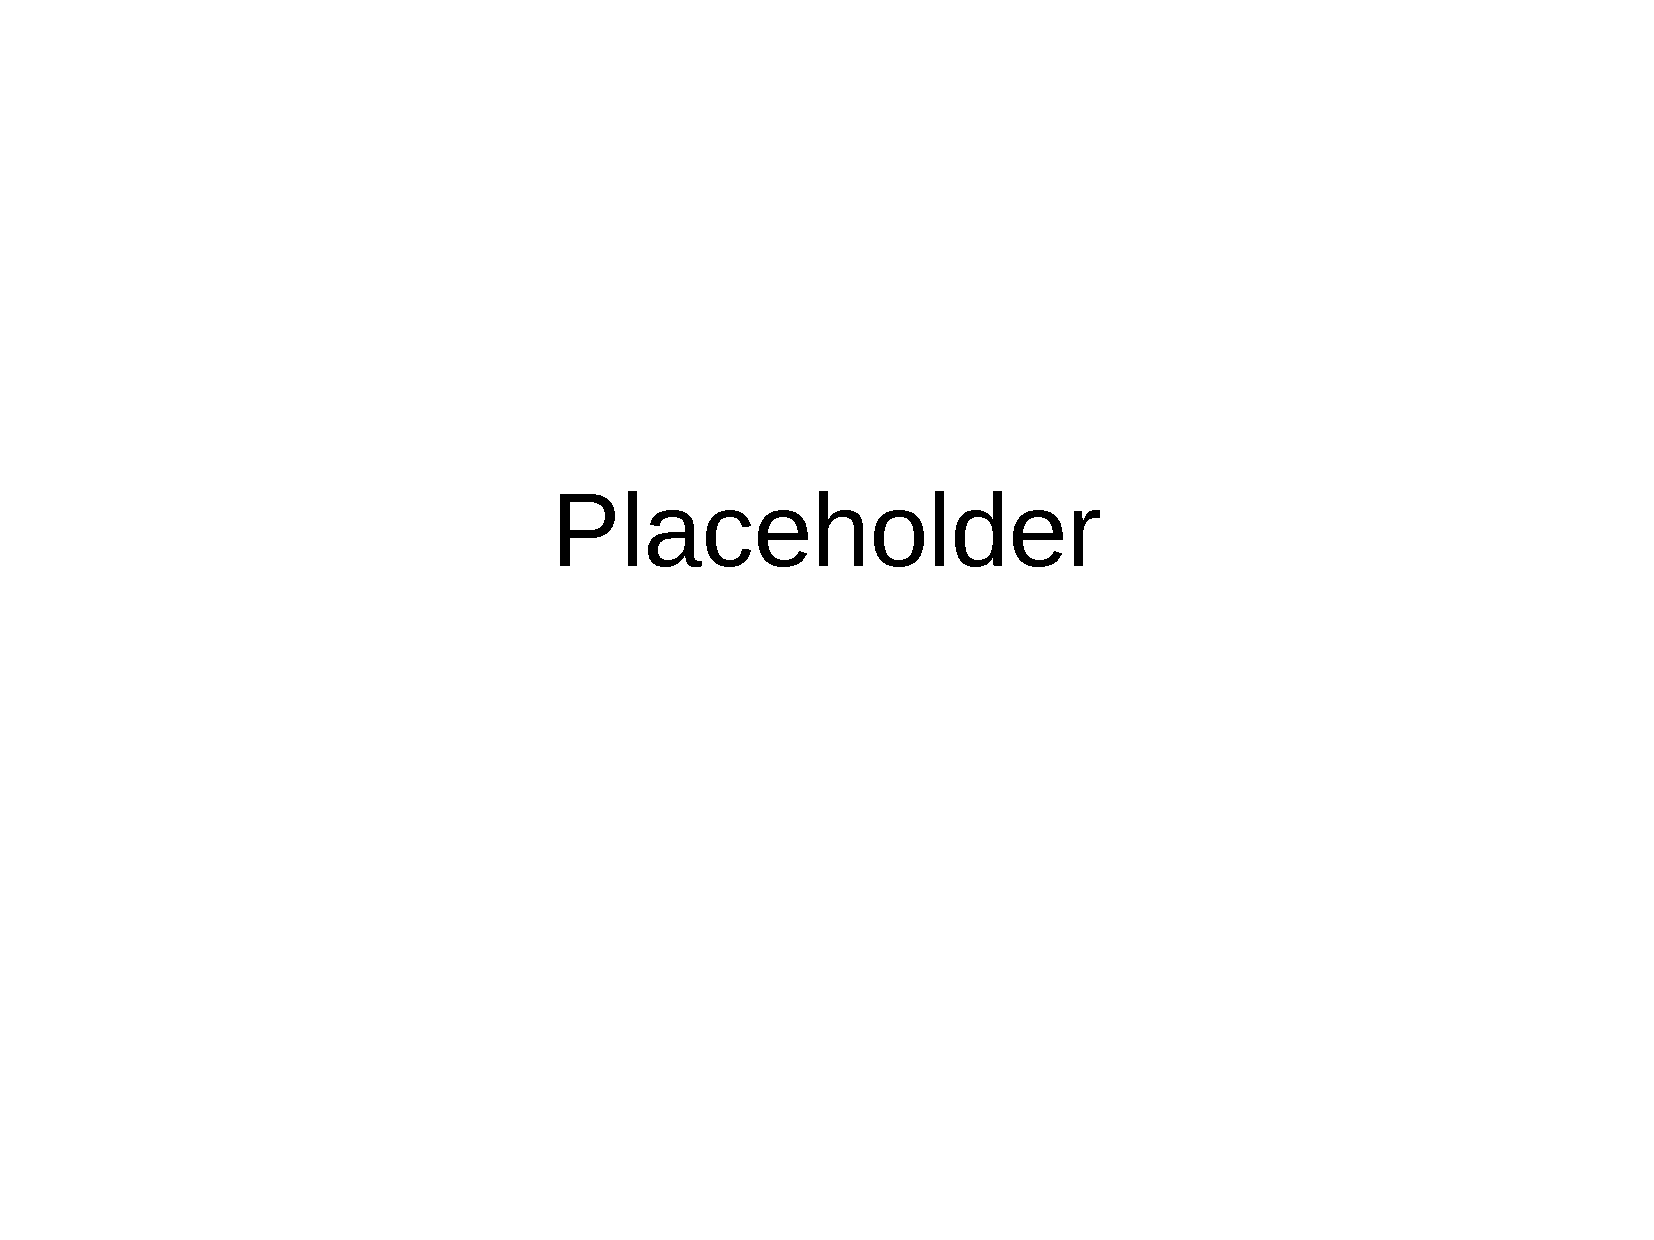
\includegraphics[width=\textwidth]{placeholder}
	\caption{Signal vs noise after imrpoving the readout chain.}
	\label{fig:viper_snr-good}
\end{figure}
\chapter{Charge readout studies\label{chap:charge-ro}}


\section{A more robust approach to TPC readout wires\label{sec:charge-ro_cuoka}}

As outlined in Section~\ref{sec:lartpc_challenges}, one of the big challenges for future \lartpc s will be the mechanical stability of the classical wire readout planes for the envisioned detector sizes.
A possible solution to the mechanical problems with wires is to not use actual wires but instead print thin coper tracks on a support structure.
To investigate this solution, a proof of concept was performed at LHEP at the University of Bern.


\subsection*{Experimental setup}

In a classical wire readout plane, the induction signal is produce by drifting the charge through one or multiple induction wire grids.
With the proposed scheme of \si{Cu} tracks on a support structure, it is no longer possible for the charge to actually drift through the induction plane(s).
Therefore, induction is only produced by the approach of the charge.
One consequence of this is, that induction signals will no longer bi bipolar.
As opposed to the classic design, the collection plane will even be in front of the induction plane(s).
This means that the charge can only approach the induction plane(s) until it is collected by the collection plane on the top layer of the support structure.
That is why it is crucial to make the support structure as thin as possible in order to get induction signals as high as possible.
Using an FR4 structure as in classical PCB designs is therefore not a viable option.
Very thin support structures can be provided by using a flexible PCB made from Kapton instead of FR4.
These can be made as thin as a few \SI{10}{\micro\metre}.
For this test, a Kapton layer of \SI{50}{\micro\metre} was used with a single induction plane on the back (Fig.~\ref{fig:cuoka_readout-plane}).
The Kapton layer was supported by an FR4 frame for mounting on the TPC.

\begin{figure}[htb]
	\centering
	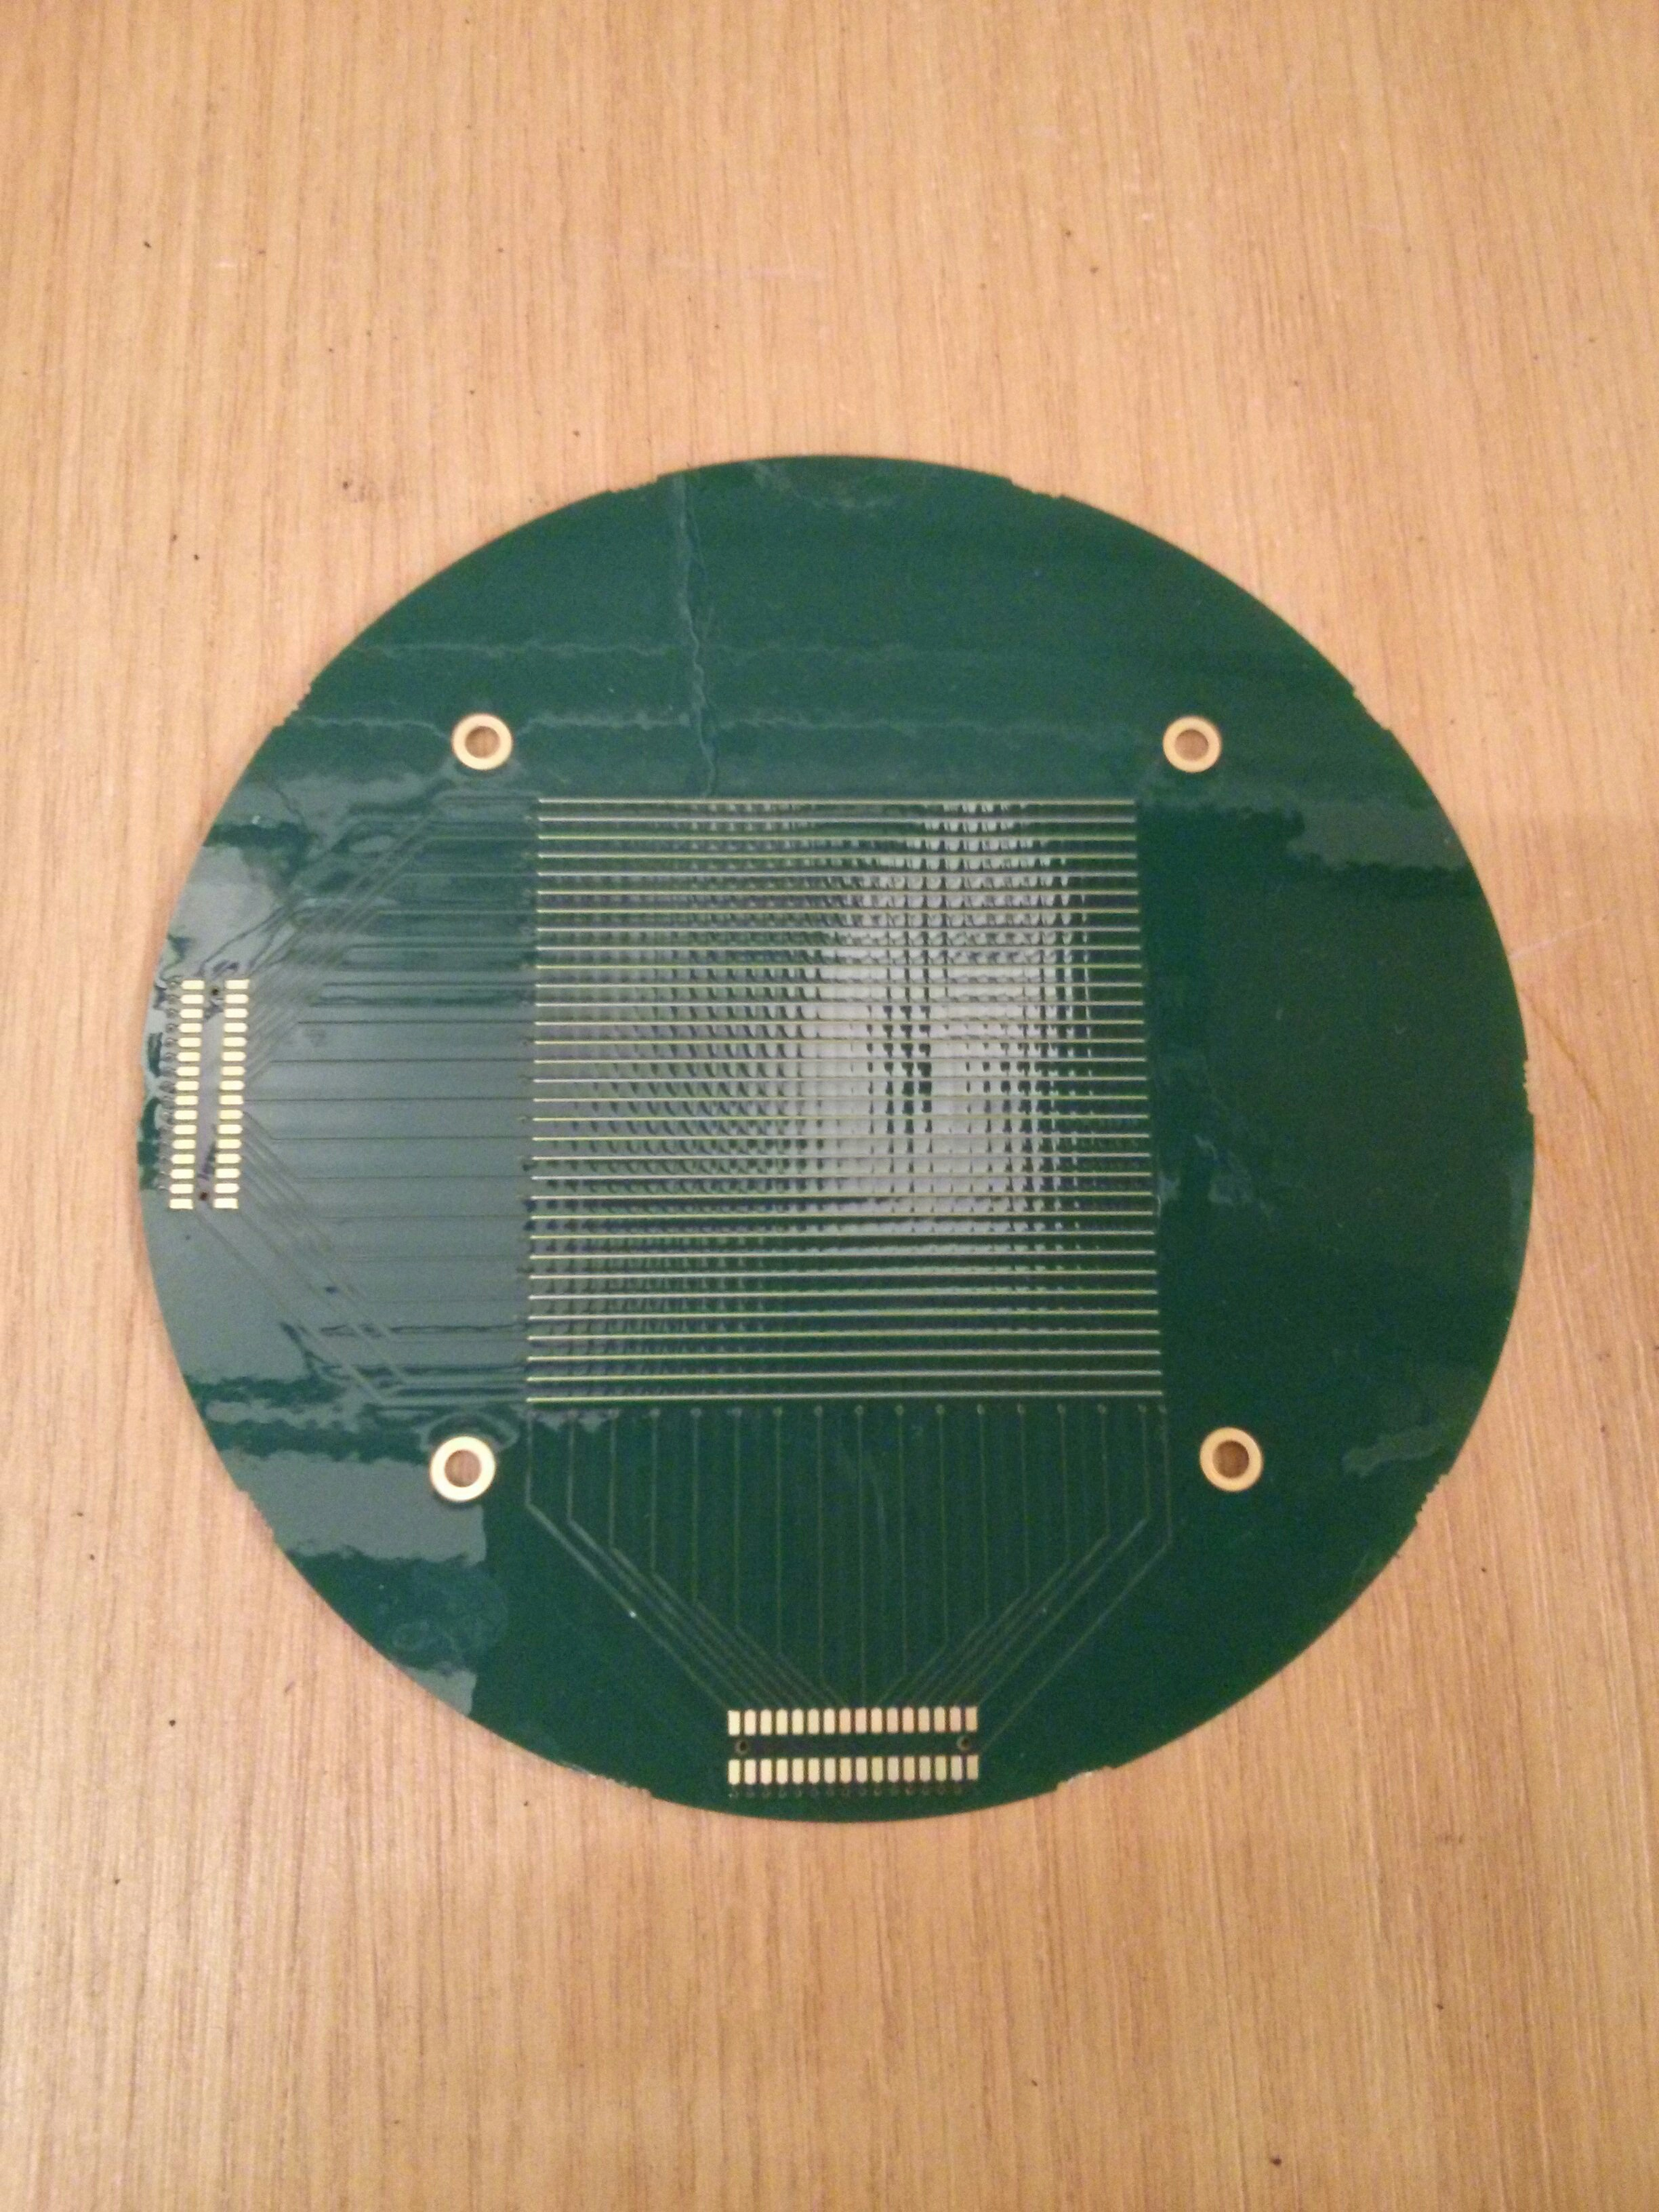
\includegraphics[width=0.5\textwidth]{cuoka/readout_plane_bottom}
	\caption{Copper on Kapton readout plane.}
	\label{fig:cuoka_readout-plane}
\end{figure}

The test was performed in a small vacuum-insulated double-batch cryostat with an inner volume of \SI{30}{\centi\metre} diameter and \SI{50}{\centi\metre} height. %TODO: check dimensions!
Prior to filling, the cryostat was evacuated using a turbo-molecular pump and then purged with argon gas and evacuated a second time.
From earlier experiments the purity can be assumed to be of the order of \SI{1}{ppb} after filling.
The cryostat is sealed using rubber o-rings which lose tightness at cryogenic temperatures.
Therefore, and due to the fact that no purification system was available, the purity degraded slowly in the course of the experiment.
The \SI{8}{\centi\metre} long field cage consists of \num{8} copper rings of \SI{8}{\centi\metre} diameter terminated by a copper plate cathode.
A field of \SI{1}{\kilo\volt\per\centi\metre} is generated using a resistive divider.

\begin{figure}[htb]
	\centering
	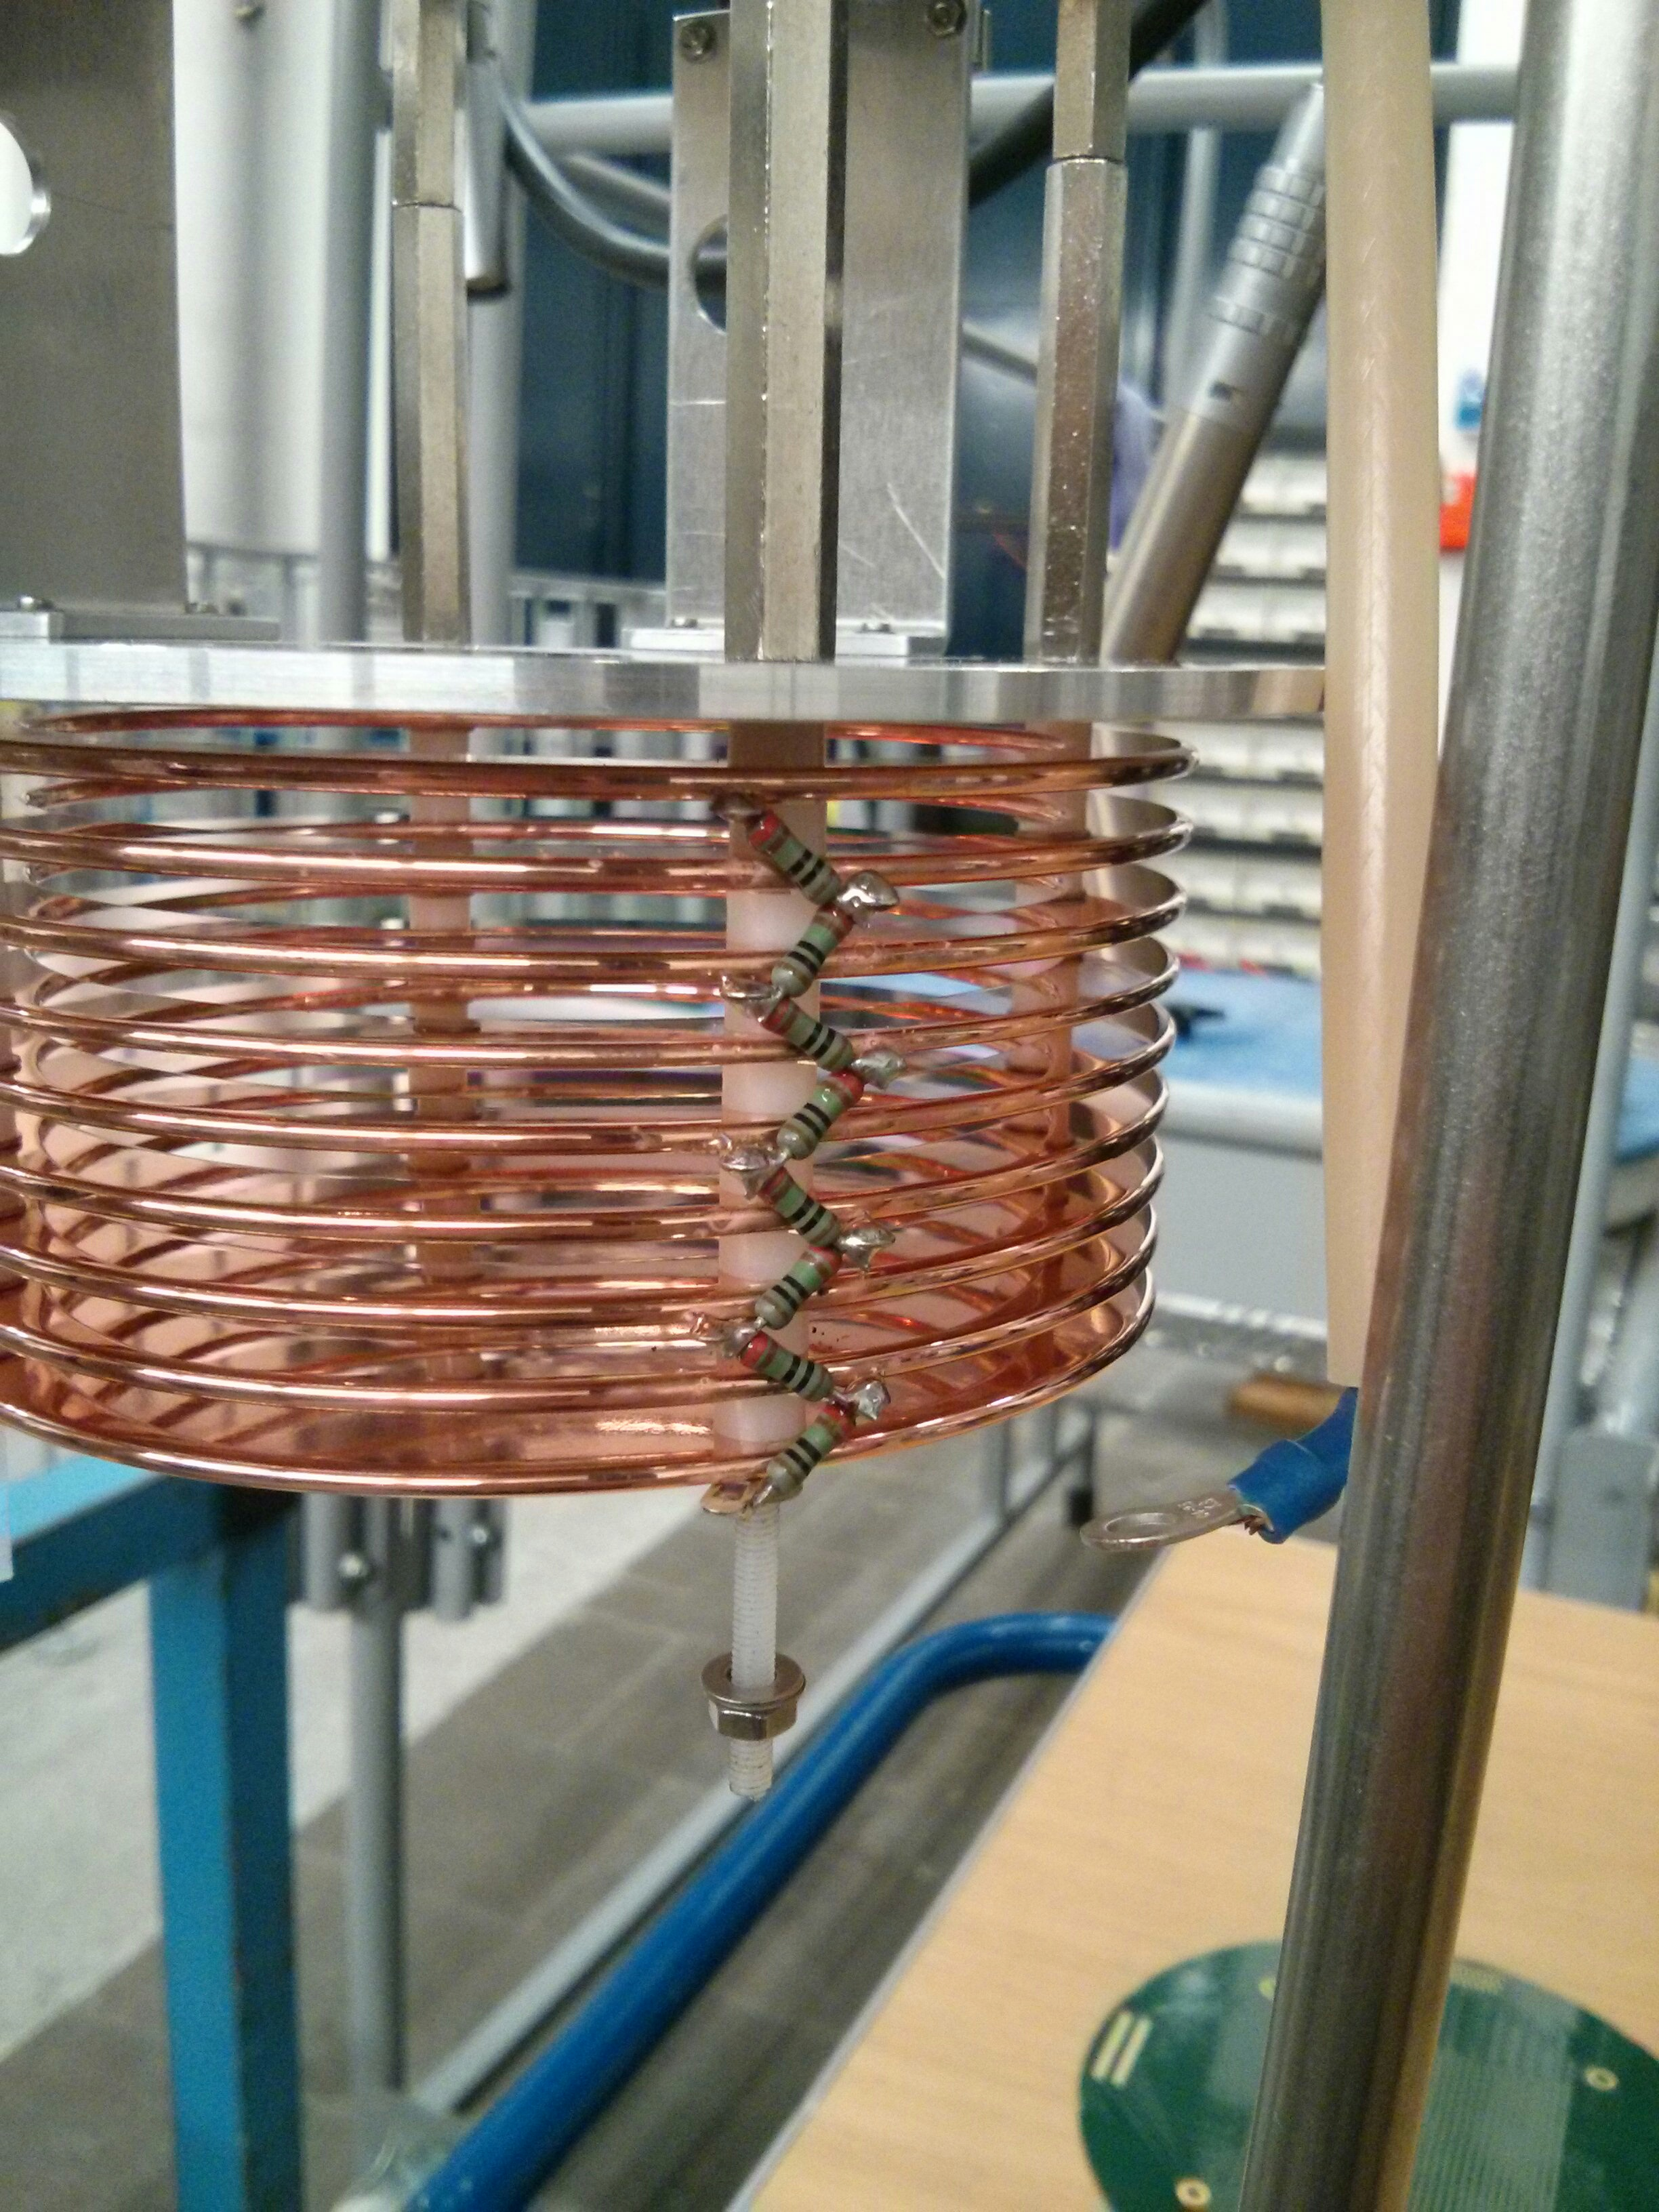
\includegraphics[width=0.5\textwidth]{cuoka/tpc}
	\caption{TPC used for the copper on Kapton readout test.}
	\label{fig:cuoka_tpc}
\end{figure}

The charge signal is amplified by cryogenic charge amplifiers.
The amplified signal is then digitised by \emph{CAEN V1724}\footnote{\href{http://www.caen.it}{http://www.caen.it}} \SI{14}{bit} digitisers.
Section~\ref{sec:electronics_existing} describes the readout chain in more detail.


\subsection*{Experimental results}

Using the above-described setup, cosmic muons were recorded over the course of multiple hours.
A typical event is depicted in Figure~\ref{fig:cuoka_event}.
It can be seen that due to the event being almost parallel to the induction strips, the induction signal is in fact stronger than the collection signal.
The reason for the bad signal to noise ratio is improper grounding of the setup and high noise levels in the lab from the nearby train station and air conditioning.
Due to time constraints and an upcoming test of a pixelated readout described in Chapter~\ref{chap:rd-dune-nd}, no analysis was performed on these data.
Anyhow, the fact that cosmic muons could be seen using this setup proofs that there is no inherent problem with having the induction plane a few \SI{10}{\micro\metre} behind the collection plane.

\begin{figure}[htb]
	\centering
	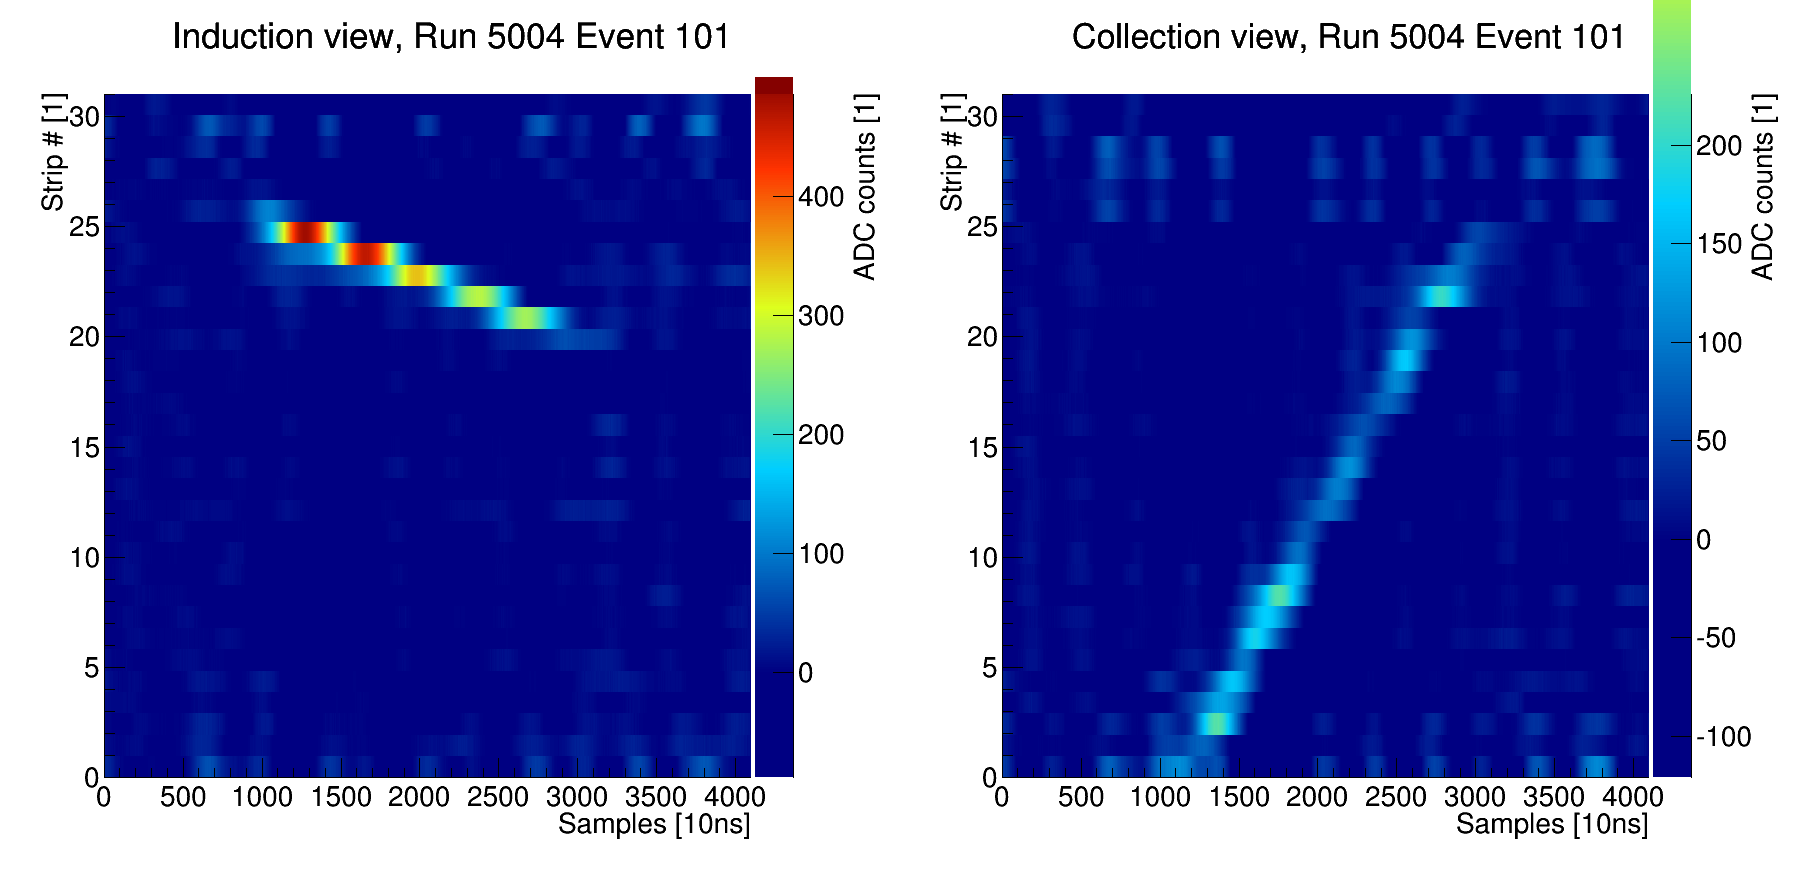
\includegraphics[width=\textwidth]{cuoka/muon_event}
	\caption{Muon event recorded using the copper on Kapton readout.}
	\label{fig:cuoka_event}
\end{figure}

While this technique can potentially solve the mechanical problems of classical wire readouts, it does not reduce the ambiguities inherent to 2D-projective readouts outlined in Section~\ref{sec:lartpc_challenges}.
Because of this, it was decided not to further investigate copper on Kapton readouts and instead focus on pixelated readouts for \lartpc s providing real 3D data.


\section{Pixel readout\label{sec:charge-ro_pixels}}
As outlined in Section~\ref{sec:lartpc_challenges}, wire readouts are not suitable for \lartpc s the size of the envisioned future neutrino detectors.
The ambiguities caused by the nature of wire readouts can be eliminated by using a fully pixelated readout.
Such a readout will record a true 2D image of the charge for every time slice and thus directly produce 3D space points of the event.
On the other hand, this will increase the required number of DAQ channels and therefore the data throughput.
To illustrate this, let us imagine a readout plane of \SI{1 x 1}{\metre} and a desired resolution of \SI{5}{\milli\metre}.
For a conventional wire readout with two planes, this results in

\begin{IEEEeqnarray}{rCl}
	\left(\frac{\SI{1}{\metre}}{\SI{5}{\milli\metre}}\right) \times 2 & = & 40
\end{IEEEeqnarray}

wires and thus DAQ channels.
In order to reduce ambiguities, one can use more than two planes which will increase the number of channels linearly with the number of planes.
For a pixelated readout,

\begin{IEEEeqnarray}{rCl}
	\left(\frac{\SI{1}{\metre}}{\SI{5}{\milli\metre}}\right) ^ 2 & = & 400
\end{IEEEeqnarray}

DAQ channels are required.
Scaling this up to the needed detector size, this leads to an enormous number of DAQ channels and data throughput.

It is possible to reduce the number of channel by employing some form of multiplexing.
There are multiple options, one could imagine for this:
\begin{itemize}
	\item Digital multiplexing
	\item Analogue multiplexing
	\item Genetic multiplexing
	\item Regions of interest
\end{itemize}

Digital multiplexing means digitising all channels as close as possible to the readout plane and then mutliplexing the digital data onto a high-speed digital link.
An advantage of this technique is that the technology for this already exists and is well established in information technology.
Ideally, one would feed the data stream into an optical fibre which additionally would provide galvanic isolation of the readout from the DAQ.
The challenging part is that all of this needs to happen at cryogenic temperatures which is far from trivial because most off-the-shelf components are not made for this.

Analogue multiplexing is similar to digital multiplexing but multiplexes the signals into an analogue link before digitising them at room temperature outside the cryostat.
While no digital circuits at cryogenic temperatures are needed, there is still a need for an analogue multiplexer and it is not given that this is any easier to realise than a digital one.

Genetic multiplexing is a technique which connects multiple pixels to one DAQ channel.
The connections are done in a way that from the pattern of channels activated by a certain event type (a single straight track for instance), it is possible to recover the correct pixel that was hit.
Naturally, this reintroduces new ambiguities.
Depending on the complexity of the event topology and the number of pixels multiplexed to one channel, it is possible or not to resolve them during reconstruction.
In any case, if the event is too complex, it cannot be reconstructed properly.
While genetic multiplexing has been shown to work for one-dimensional readouts, there is no known solution for two dimensions. %TODO: sauce

A fourth technique is to subdivide the readout plane in so-called regions of interest or ROIs.
This scheme was tested for an earlier PhD thesis at LHEP at the University of Bern using Micromegas in a xenon gas TPC~\cite{maplesyrup}.
All pixels at the same position inside the ROIs are connected to the same DAQ channel.
For instance, let us assume squared regions of interest.
One DAQ channel would connect to all the pixels in the top left corners of the ROIs.
Another channel would connect to all the pixels in the top right corner and so on.
To explain this a little better, let us assume a square pixel plane of $N \times N$ pixels where $N = n ^ 2$ with an arbitrary integer $n$.
Now, we divide the plane into $n \times n = N$, each consisting again of $n \times n = N$ pixels.
For such a readout, we require $N$ DAQ channels for the ROIs and another $N$ channels for the pixels.
We need only as many pixel channels as we have pixels per ROI because all the pixels at the same relative position inside the ROIs are connected together to one DAQ channel.
This means that we can read out a $N \times N$ pixel plane using only $2 N$ DAQ channels; the same number required by a conventional 2-plane wire readout of the same size and pitch.
If there is a signal on a certain DAQ channel, the position inside the ROI is known but not the ROI.
To determine the full position, each ROI has its own inductive grid in between the pixels.
The grid is biased such that the charge is fully focussed onto the pixels and does not collect any charge.
Combining the bipolar pulse on the ROI grid with the collection pulse from the pixels, it is possible to disentangle the true position.
Again, the drawback of this approach is that it is not free of ambiguities.
It fails for multiple simultaneous hits when it is impossible to say which pixel pulse belongs to which ROI pulse.

Independently of the amount of data one needs to bring out of the detector, a second problem is heat dissipation.
The more of the readout chain is sitting inside of the detector, the more serious this problem becomes.
It is especially problematic for digital multiplexing which requires a lot of cryogenic electronics.
A possible solution to this is to power only that part of the readout that is actually needed.
This would require a means to wake up the part of the readout where the charge is arriving before it is collected.
Provided, the wake-up time is short enough, inductive grids on regions of interest could allow precisely for this.

Because it has already been successfully tested in a gas TPC, the region of interest approach was chosen for the first prototype of a pixelated \lartpc.
A readout plane fitting the TPC described in Section~\ref{sec:viper_setup} was designed.
Because the detector is a single-phase \lartpc, and thus no gas amplification as in Micromegas is needed, the readout plane could be realised as a conventional PCB.
It consists of \num{28} regions of interest each one of which is made of \num{6 x 6} pixels.
This means that \num{36} DAQ channels are required to acquire the pixel signals plus another \num{28} channels for the ROI signals, resulting in a total of \num{64} DAQ channels to readout $28 \times 36 = 1008$ pixels.
The pixels are \SI{900}{\micro\metre} vias with a pitch of \SI{2.86}{\milli\metre} while the inductive grids are made from \SI{152.4}{\micro\metre} copper tracks.
\chapter{Light Readout Studies\label{chap:light-ro}}


\section{SiPM Light Readout\label{sec:rd-dune-nd_light}}

For the \AC\ detector concept detailed in Chapter~\ref{chap:argoncube}, a slim and efficient light readout is needed.
Photomultiplier tubes (PMTs) are not suitable because they occupy a lot of space and thus would require mounting on top of a module which in turn would reduce their efficiency.
That is why the photon detectors of choice for such a detector are silicon photomultipliers (SiPMs).
In 2016, LHEP at the University of Bern developed a novel cosmic ray tagger system for \lartpc s which was subsequently installed in the MicroBooNE experiment~\cite{uboone} and will be installed in the SBND experiment~\cite{sbnd} in the near future.
The tagger consists of panels made from polystyrene based scintillating bars.
On both long edges of the strips, the light is coupled into a \emph{Kuraray Y11(200)M}\footnote{\url{http://kuraraypsf.jp}} wavelength-shifting (WLS) fibre of \SI{1}{\milli\metre} diameter.
One end of the fibre is coated with an aluminium mirror to increase collection efficiency.
The other end is attached to a \emph{Hamamatsu S12825-050P}\footnote{\url{http://www.hamamatsu.com}} silicon photomultiplier (SiPM).
A bespoke front-end board (FEB) reads out the SiPM signal and provides power.
It was developed at LHEP at the University of Bern alongside the scintillator panels\cite{crt_feb}.

For the first prototype, the CRT system was adapted to serve as the light trigger system.
Except for operating everything up to the SiPMs in liquid argon, the polystyrene scintillating bars were replaced by acrylic rings.
The latter are placed in between the aluminium field shaping rings.
To allow for proper convection of the liquid argon, only every other gap is completely filled by an acrylic ring.
Perpendicularly to the rings(i.e.\ in drift direction), four WLS fibres collect the light from the rings and guide it to the readout plane on the anode side where it is fed to the SiPMs.
Residing on the cryostat top-flange at room temperature, the front-end board is connected to the SiPMs via Teflon insulated coaxial cables.

The peak of scintillation light emission in liquid argon lies at \SI{128}{\nano\metre}~\cite{sauce} while the sensitivity wavelength peak of the SiPM is at \SI{450}{\nano\metre}.
Therefore, the scintillation light needs to be shifted before it can be detected by the SiPMs.
This happens in two stages.
For the first shift, tetraphenyl butadiene (TPB) is applied to the inside of the acrylic rings.
Their outside is not coated to reduce the collected amount of scintillation light that originates outside the TPC.
TPB absorbs the \SI{128}{\nano\metre} scintillation light an re-emits with a peak at \SI{440}{\nano\metre}~\cite{tpb} which is then propagated through the acrylic and coupled into the WLS fibre.
The latter has an absorption peak at \SI{430}{\nano\metre} and an emission peak at \SI{476}{\nano\metre}.

In the front-end board, two coincidences of two out of four SiPMs are formed and combined by means of a logic \emph{OR} operation.
The trigger pattern is thus

\begin{IEEEeqnarray}{rCl}
	T & = & \qty(S_1 \land S_2) \lor \qty(S_3 \land S_4)
\end{IEEEeqnarray}

for SiPMs $S_1$ through $S_4$.
The reason for this is that the same trigger logic is used for the CRT panels to have a coincidence between two fibres of one scintillation bar.
In order to improve trigger purity, it was tried to change the firmware to trigger on the coincidence of all four fibres in the TPC but this could not be achieved due to a firmware bug.
\chapter{Results from the First Measurements with the \AC{} Pixel Demonstrator}
\label{chap:viper}


\section{Pixel PCB Design}
\label{sec:viper_PCB}
 
The pixelated anode plane, shown in Figure~\ref{fig:viper_pixies}, was produced as a conventional Printed Circuit Board (PCB). 
The pixelated area is \SI{100}{\milli\metre} across, the pixels are formed of \SI{900}{\micro\metre} vias with a pitch of \SI{2.54}{\milli\metre}.
An inductive focusing grid surrounds the pixels, it is made from \SI{152.4}{\micro\metre} copper traces split into 28 regions.
There are \num{6 x 6} pixels per region, giving a total of 1008 pixels. 

\begin{figure}[htb]
	\centering
	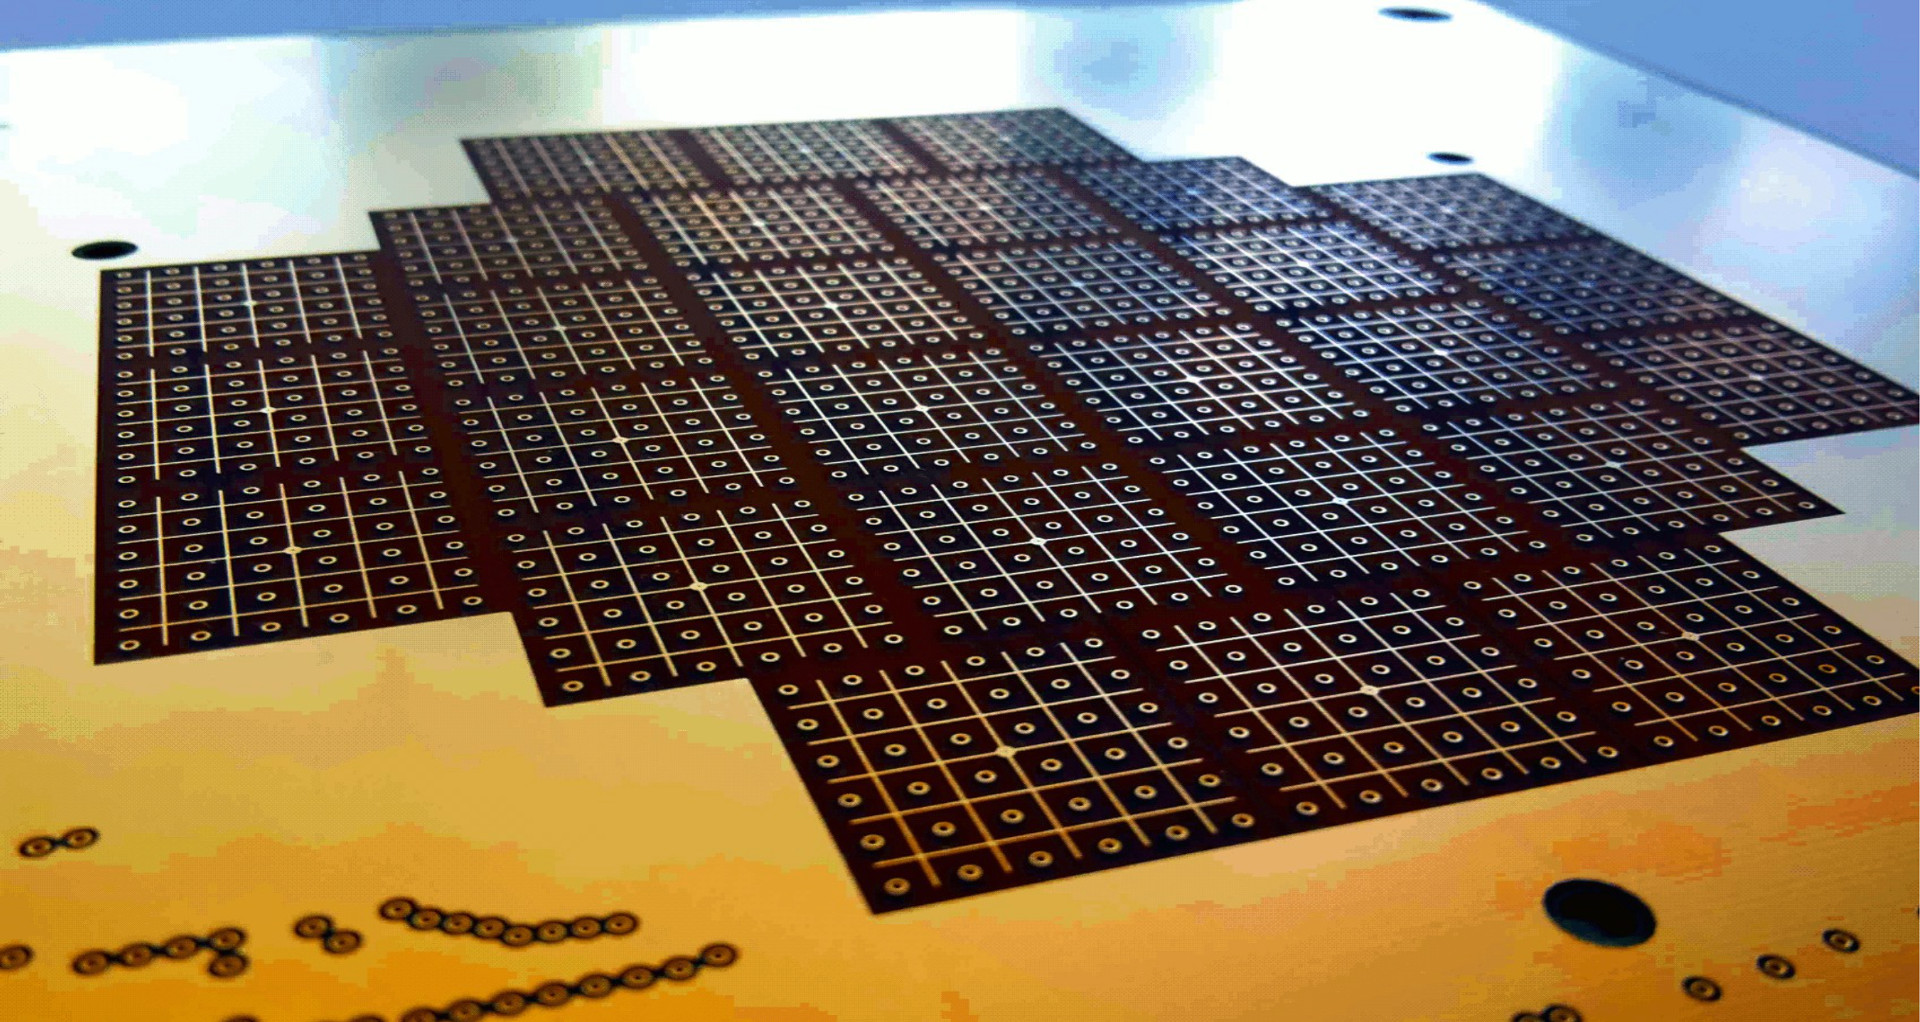
\includegraphics[width=0.65\linewidth]{viper/pixies}
	\caption{Initial (July 2016) pixelated anode PCB. The pixelated readout area is \SI{100}{\milli\metre} in diameter.
	Each charge collection pixel is a \SI{900}{\micro\metre}, at a pitch of \SI{2.54}{\milli\metre}, inductive focusing grids formed of \SI{152.4}{\micro\metre} copper traces surround the pixels.
	There are 28 inductive focusing grids with 36 pixels per region, a total of 1008 pixels.}
	\label{fig:viper_pixies}
\end{figure}

Vias were used for pixels instead of pads in order to minimise capacitance.
It is important that capacitance is minimised when amplifying charge as thermal noise scales with capacitance: $Q_{\mathrm{Noise}}=\sqrt{k_{\mathrm{B}}TC}$~\cite{noise}.
To further minimise parasitic capacitance, the PCB design was optimised by removing unnecessary ground planes, routing signal tracks outside necessary ground planes, and increasing the thickness of the PCB to \SI{3.5}{\milli\metre} from an initial \SI{1.75}{\milli\metre}. 
Capacitance at each pixels is $\order{\SI{50}{\pico\farad}}$.

The pixels are directly connected to the preamplifiers while the inductive focusing grids are decoupled via \SI{10}{\nano\farad} capacitors.
Additionally, the bias voltage is filtered at the input by another \SI{10}{\nano\farad} and \SI{10}{\mega\ohm}.
The full schematic of the bias circuit is depicted in Figure~\ref{fig:viper_pcb_schematic}.

\begin{figure}[htb]
	\centering
	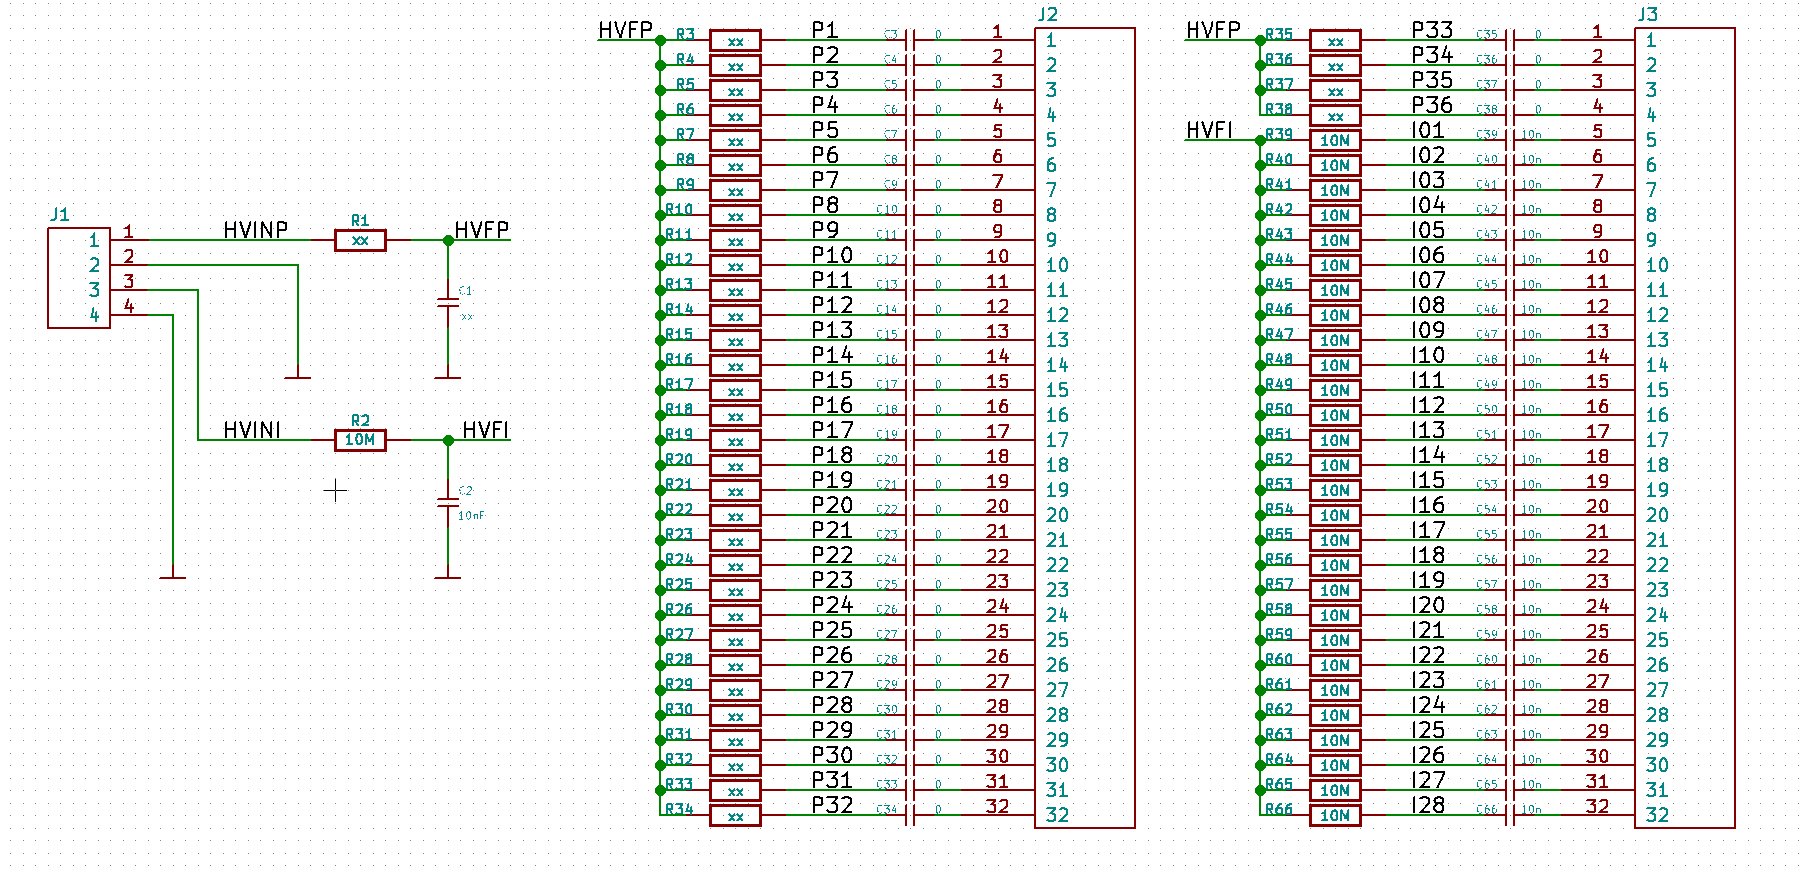
\includegraphics[width=\textwidth]{viper/pixel_pcb_schematic}
	\caption{Schematic of the bias circuit for the \AC{} pixel demonstrator PCB.
	On the left, the pinheader connected to the bias HV power suplly is shown. In the middle and on the right are the connections to the pixels and inductive ROI grids.
	The connections to the preamplifier inputs are located at the positions of numbers P1--P36 (pixels) and I1--I28 (ROIs).
	For simplicity and universality, the same circuit was used for both pixels and ROIs eventhough for the measurements described in this work, only the inductive ROI grids were biased.
	Therefore, the ROIs are connected as depicted (R2 and R39--R66, C2 and C39--C66).
	As the pixels need not be biased, they are directly connected to the preamplifiers by leaving R3--R38 unpopulated and replacing C3--C38 by \SI{0}{\ohm} resistors.
	Additionally, R1 is \SI{0}{\ohm} and C1 unpopulated, and by connecting pin 1 of J1 to ground, all unused PCB traces are grounded.}
	\label{fig:viper_pcb_schematic}
\end{figure}

The bias on the inductive focusing grids had to be sufficient to allow full charge transparency (all charge collected by the pixels), yet low enough to minimise any risk of damaging the cold coupling capacitors.
It was increased incrementally until transparency was observed at \SI{300}{\volt}. 
Simulation suggest this was only \SI{95}{\percent} transparency, with \SI{100}{\percent} at \SI{350}{\volt} (see Figure~\ref{fig:viper_transparency}).
The simulation available at the time of the measurement contained a bug resulting in an underestimation of the bias voltage required for full transparency.
During measurments, the bug became apparent and full transparency had to be estimated by looking at live data from the detector.
Due to the limited accuracy of this method, measurements were not taken up to the bias voltage for full transparency suggested by the (corrected) simulation.~\cite{francypants}

\begin{figure}[htb]
	\centering
	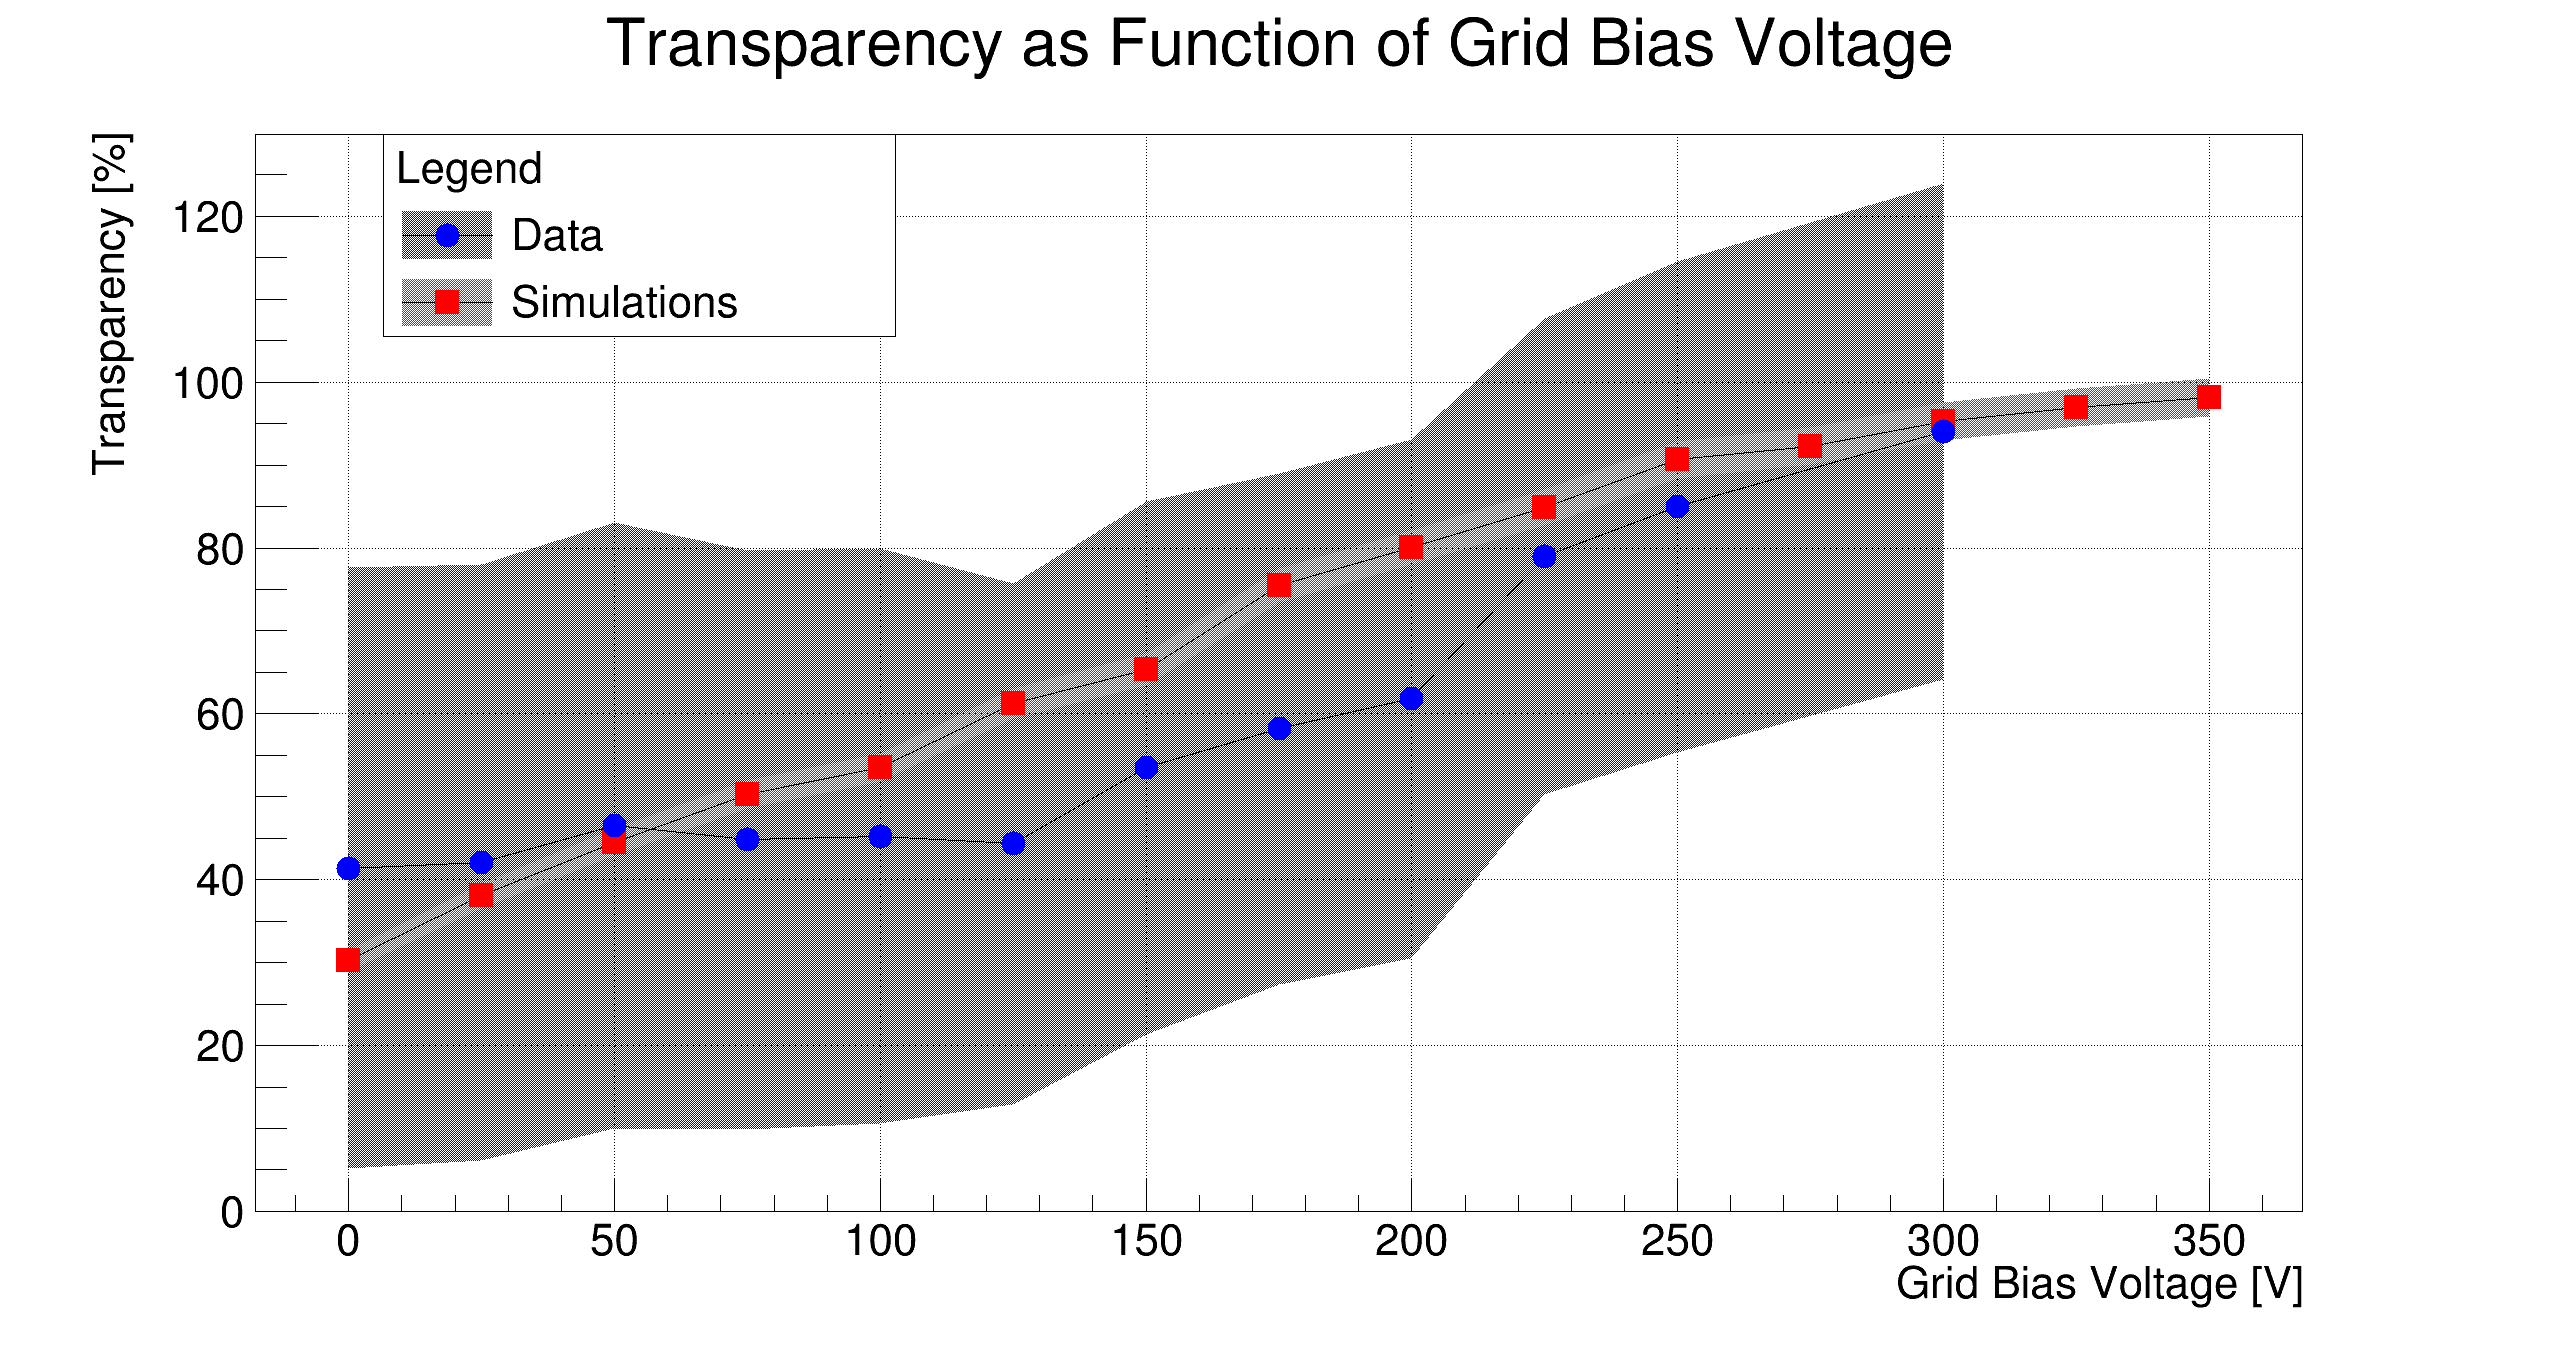
\includegraphics[width=\textwidth]{viper/transparency}
	\caption{Measured and simulated transparency versus bias voltage of the \AC{} pixel demonstrator.
	The simulation available at the time of the measurement contained a bug resulting in an underestimation of the bias voltage required for full transparency.
	During measurments, the bug became apparent and full transparency had to be estimated by looking at live data from the detector.
	Due to the limited accuracy of this method, measurements were not taken up to the bias voltage for full transparency suggested by the (corrected) simulation.~\cite{francypants}}
	\label{fig:viper_transparency}
\end{figure}


\section{TPC}
\label{sec:viper_tpc}

The pixel demonstration TPC, shown in Figures~\ref{fig:viper_cad}~and~\ref{fig:viper_v1per}, is cylindrical with an inner diameter of \SI{101}{\milli\metre} and a \SI{590}{\milli\metre} drift length. 
The TPC operated with a drift field of \SI{1}{\kilo\volt\per\centi\metre}, corresponding to a total drift time of \SI{281}{\micro\second} at \SI{2.1}{\milli\metre\per\micro\second}.~\cite{protoLASER}

\begin{figure}[htb]
	\centering
	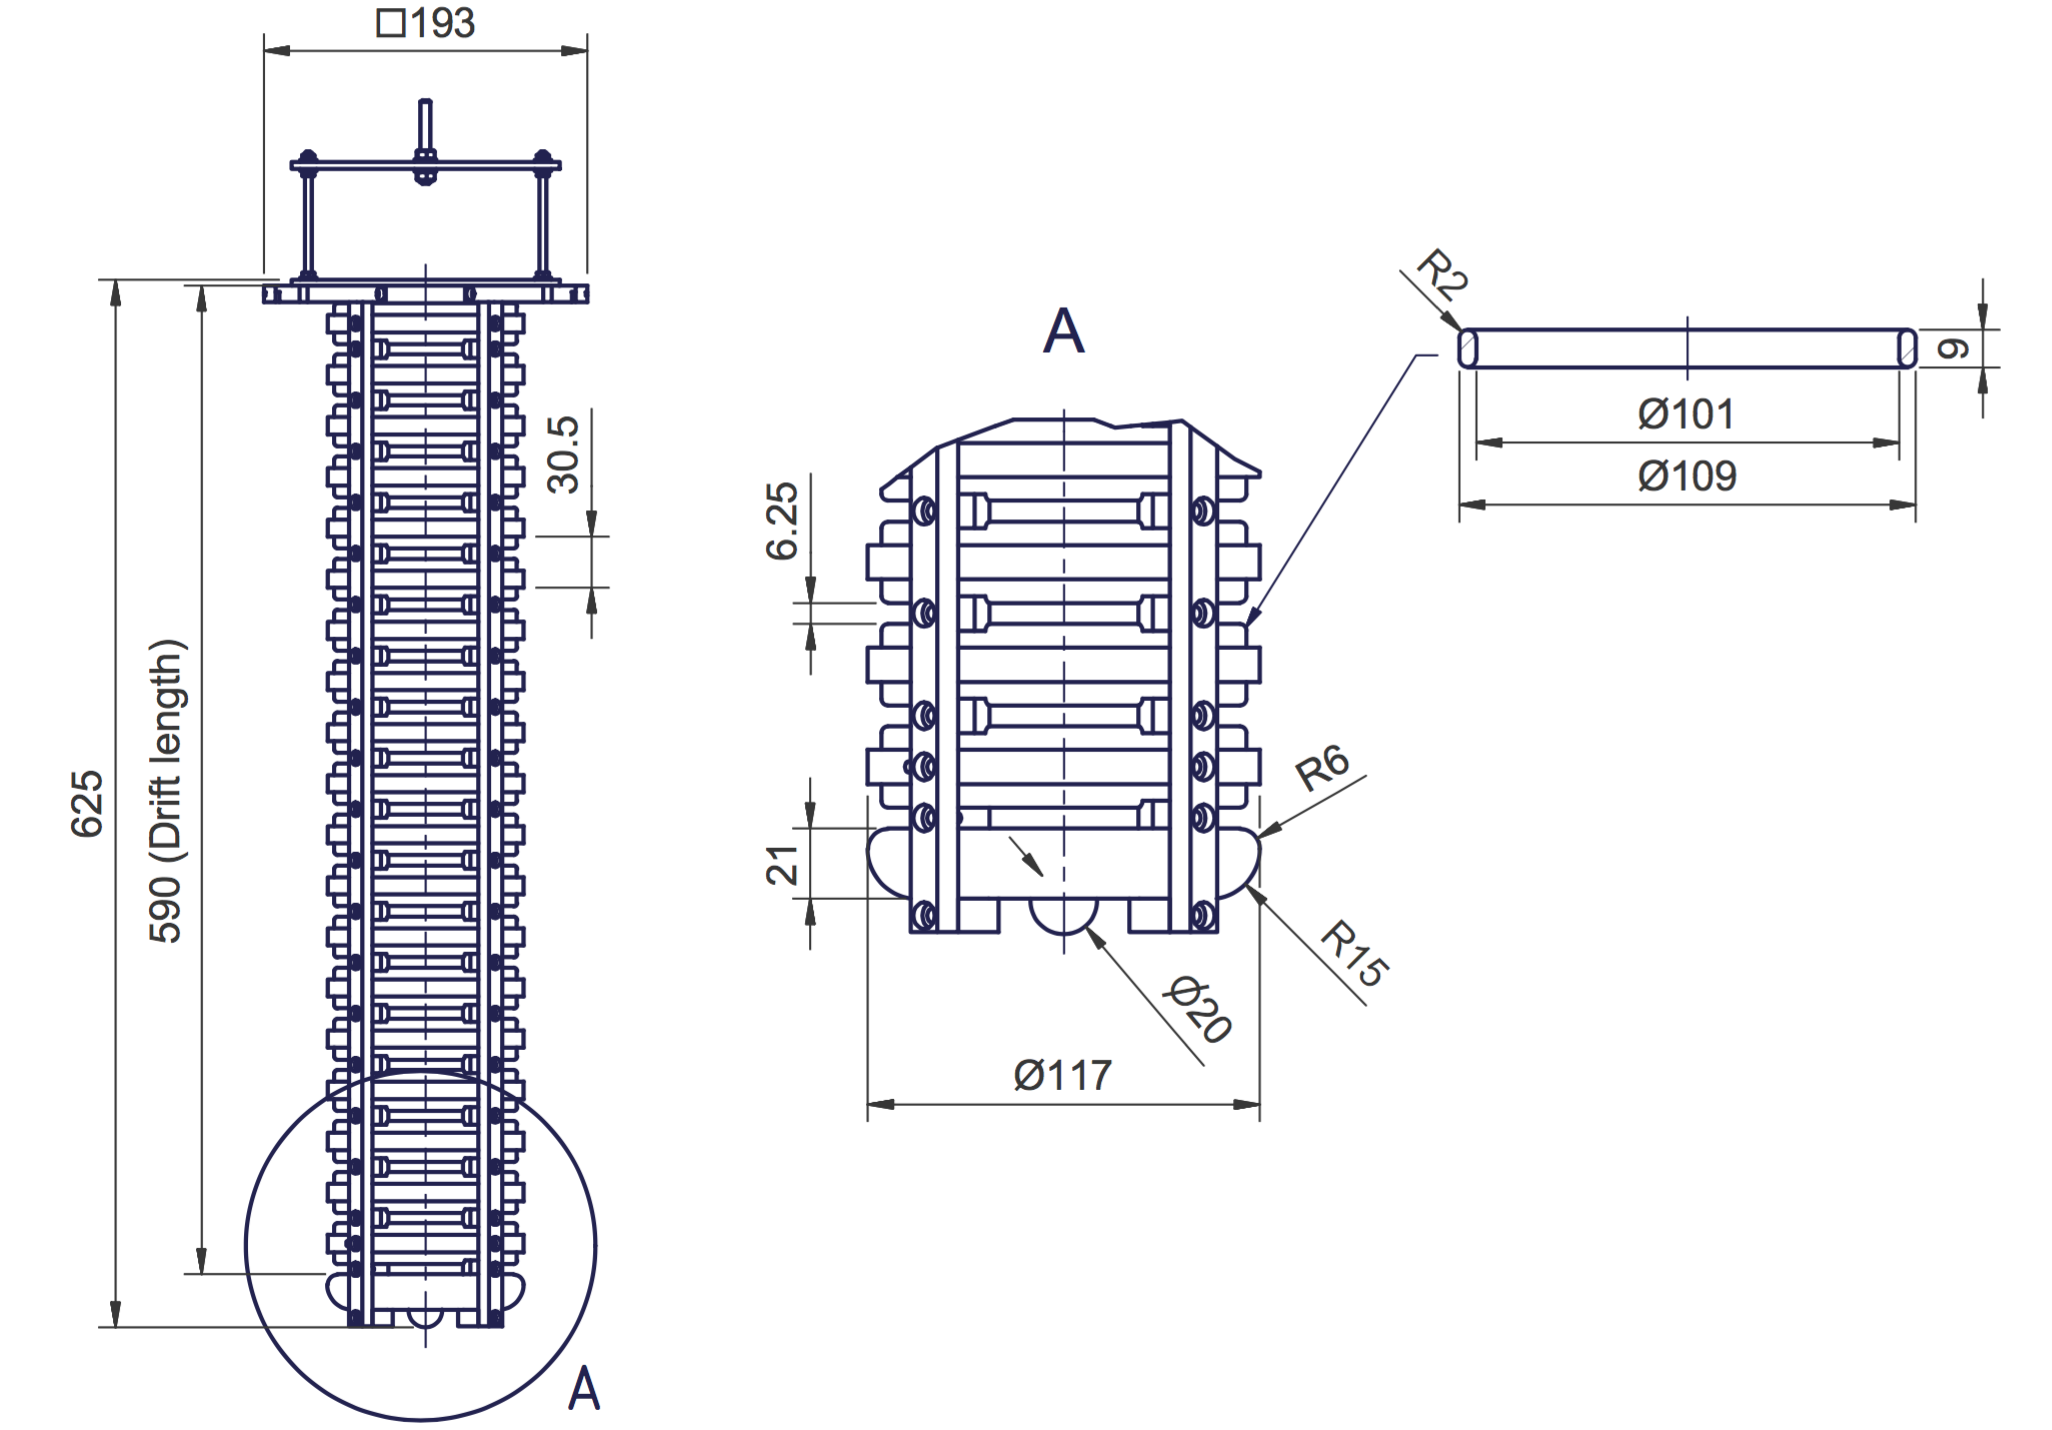
\includegraphics[width=0.9\linewidth]{viper/tpc_cad}
	\caption{\small Engineering drawing of the pixel demonstration TPC; \SI{590}{\milli\metre} drift length; \SI{6.25}{\milli\metre} field cage spacing; \SI{101}{\milli\metre} internal diameter.}
	\label{fig:viper_cad}
\end{figure}
 
The field-cage consists of aluminium rings supported by clear acrylic rings, with a cathode formed of a brass disc. 
The dimensions of the field-cage and cathode are shown in Figure~\ref{fig:viper_cad}.
Alternating acrylic rings are split, to allow for the circulation of purified LAr within the TPC volume.
Four square section PolyAmide-Imide (PAI) uprights support the cathode and field cage, with PolyEther Ether Ketone (PEEK) screws fixing the pillars to the acrylic rings.
The four PAI uprights connect to a PAI frame which supports the anode plane and the light readout Silicon PhotoMultipliers (SiPMs), see Figure~\ref{fig:viper_v1per}.   

The resistive divider consists of a chain of \SI{100}{\mega\ohm} Vishay Rox metal oxide resistors (ROX100100MFKEL).
Each resistor is soldered to its neighbour, and fixed to the field cage at each joint with an M3 screw.   

\begin{figure}[htb]
	\centering
	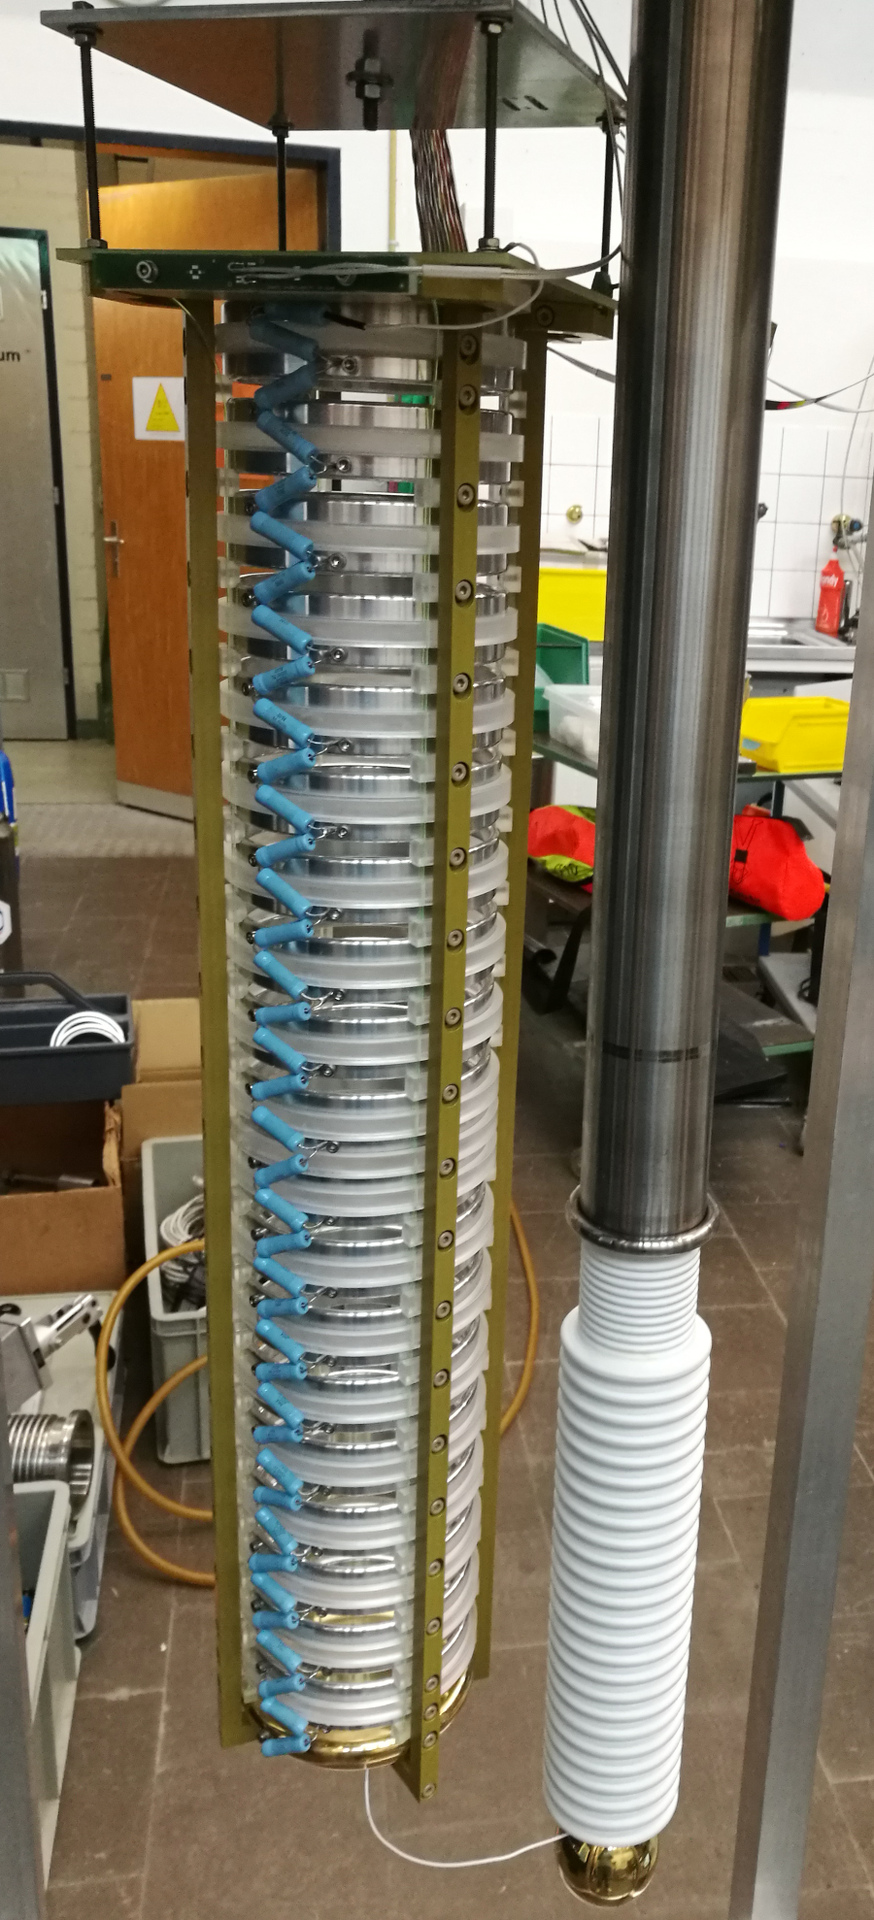
\includegraphics[width=0.26\linewidth]{viper/viper_original}
	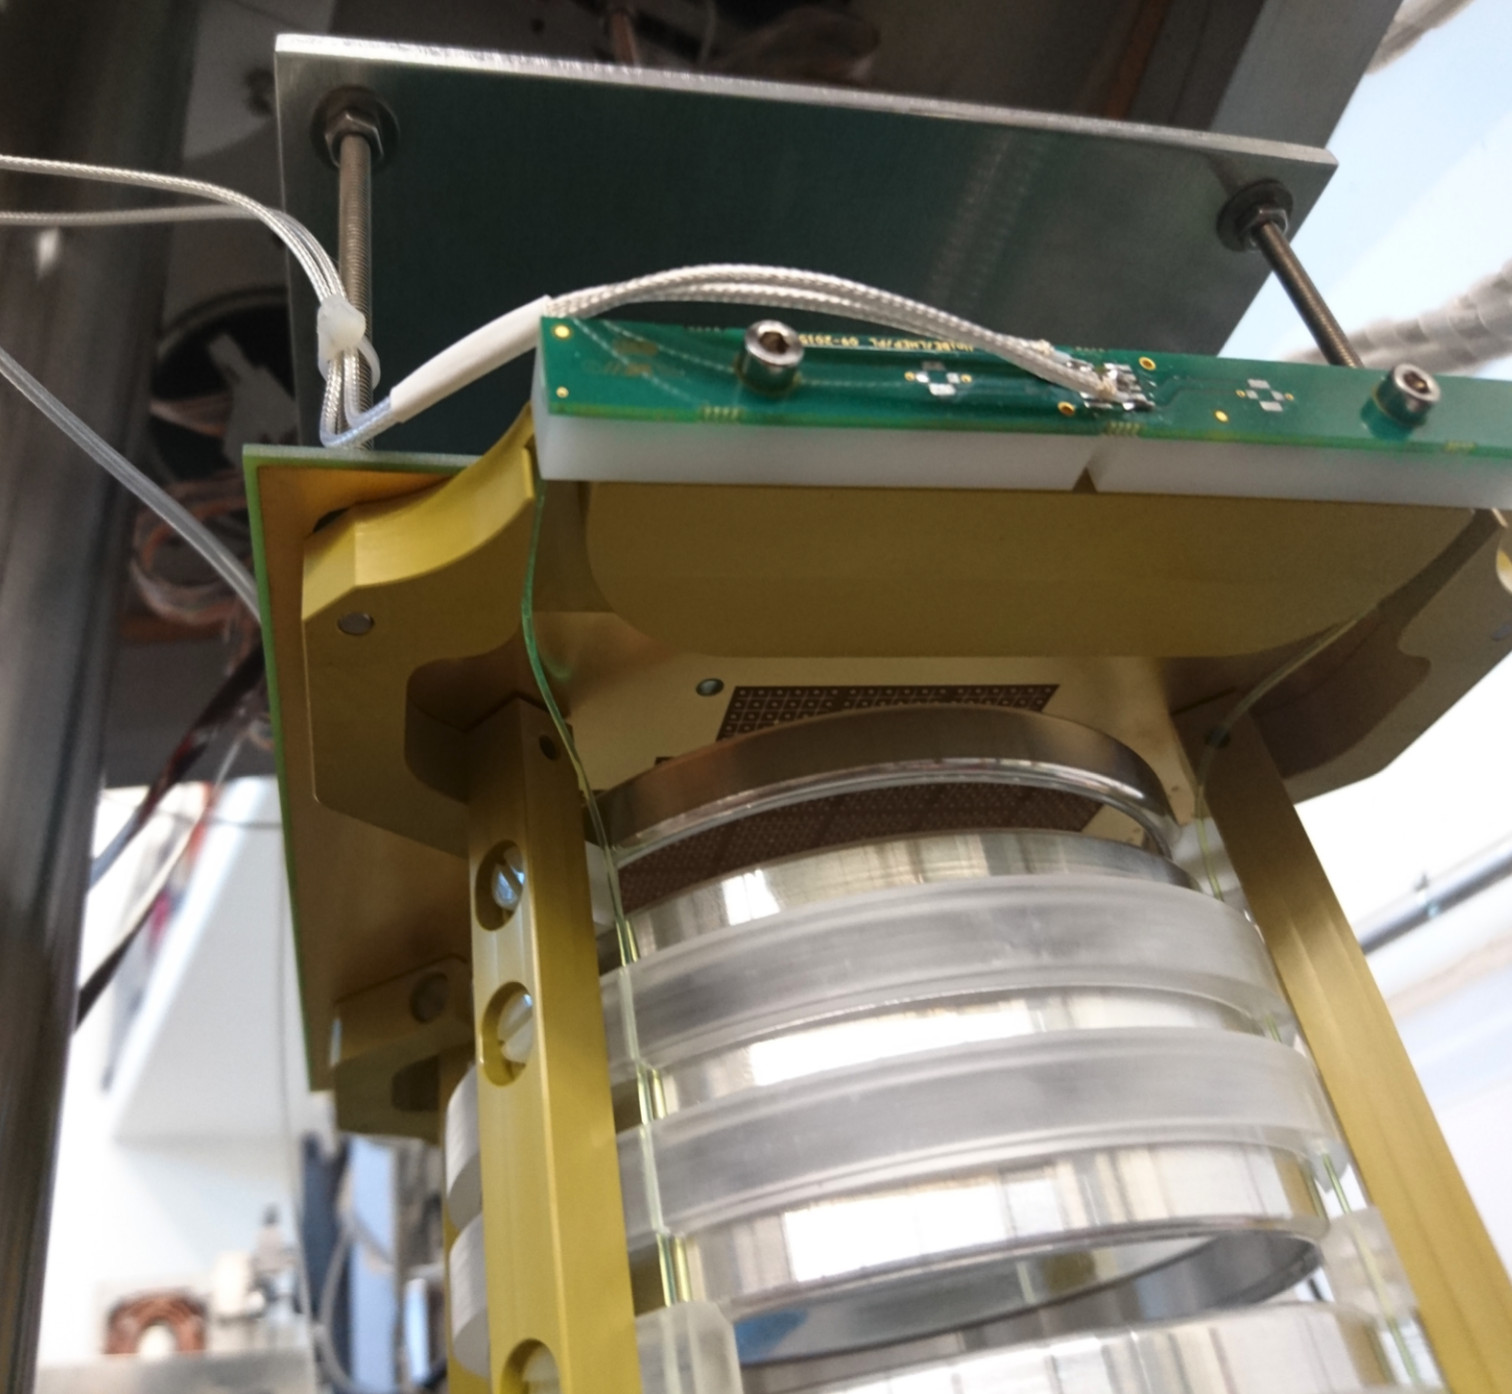
\includegraphics[width=0.62\linewidth]{viper/viper_sipm}
	\caption{\small  Left: Photograph of the  pixel demonstration TPC at Bern, with the HV feedthrough.
	Right: Close-up of the light collection system, showing wavelength shifting fibres coupling SiPMs to the TPB-coated light guides.}
	\label{fig:viper_v1per}
\end{figure}

The acrylic rings provide the light collection; their inner surfaces are machine-polished and coated with the WaveLength Shifter (WLS) TetraPhenylButadiene (TPB). 
The coating method is based on~\cite{TPBcoating}.
\SI{0.5}{\gram} of TPB and \SI{0.5}{\gram} of acrylic flakes were dissolved in \SI{50}{\milli\liter} of toluene and then mixed with \SI{12}{\milli\liter} of ethanol, which serves to increase the coating homogeneity. 
Three layers of the coating were applied by hand, with a fine brush. 

\SI{1}{\milli\metre} diameter WLS fibres (Kuraray Y11(200)M) couple the acrylic rings to the four Hamamatsu S12825-050P SiPMs mounted close to the anode, see Figure~\ref{fig:viper_v1per}. 
The SiPMs and their front-end electronics were adapted from those developed at Bern for the cosmic ray taggers used in MicroBooNE and SBND~\cite{crt, crt_feb}.
For operation in LAr, the SiPM bias voltages had to be reduce from $\approx$~\SI{70}{\volt} to \SI{53}{\volt}, in order to limit the gain.   
In the front-end electronics, two coincidences of two out of the four SiPMs are formed and combined by means of a logic \textit{OR} operation. 
This coincidence is used in order to improve trigger purity.


\section{Ancillary Infrastructure}
\label{sec:viper_infrastructure}

The pixel demonstration TPC is housed in a double-bath vacuum-insulated cryostat with the outer bath open to atmosphere.
A diameter of \SI{50}{\centi\metre} and a height of \SI{110}{\centi\metre} give an inner volume of $\approx \SI{200}{\litre}$ of liquid argon.
This is the same cryostat that was used for the HV studies described in Chapter~\ref{chap:hv}.
The LAr filtering method is the same as described in~\cite{2photonAbs}, with LAr filtered first on filling through a pair of Oxysorb-Hydrosorb filters, and then recirculated through a single custom-made filter containing both activated copper and silica gel.
LAr purity is estimated to be in accordance with~\cite{2photonAbs}, with impurity concentrations $\order{\SI{1}{ppb}}$ of oxygen-equivalent, which corresponds to a charge lifetime of \SI{290+-30}{\micro\second}.

The HV feedthrough remains unchanged from the breakdown studies (Chapter~\ref{chap:hv}); a PET-C polymer dielectric capable of potentials as high as \SI{-130}{\kilo\volt}.
A low-pass filter was added between the power supply and feedthrough, which consists of an \SI{800}{\pico\farad} decoupling capacitor grounded between two \SI{100}{\mega\ohm} resistors connected in series, i.e.\ an RC low-pass filter with an additional protection resistor at the output.
For proper insulation, the whole assembly is submerged in transformer oil.


\section{Signal to noise ratio}
\label{sec:viper_snr}

To assess the Signal to Noise Ratio (SNR), dedicated noise data was taken employing a \SI{5}{\hertz} random trigger.
The data of \num{5000} events was combined.
Subsequently, all pixel and ROI channels were combined separately and filled into respective amplitude distribution histograms.
Finally, the standard deviation of the noise was calculated by fitting a Gaussian to the amplitude distribution.
This value was used to calculate the noise for pixel and ROI channels according to
\begin{equation}
	\m{SNR} = \frac{S}{\sigma}\,\m{,}
	\label{eq:snr}
\end{equation}
where $S$ is the signal and $\sigma$ is the noise standard deviation from the Gaussian fit.
As can be seen in the left plot in Figure~\ref{fig:viper_unfilteredRawData}, one of the pixel channels is significantly noisier in comparison to others, likely caused by a broken preamplifier.
Therefore, this channel was blinded for the SNR calculations.
The resulting equivalent noise charge is \SI{1095}{\elementarycharge} for the pixel channels and \SI{981}{\elementarycharge} for the inductive ROI channels

The signal $S$ is often taken for a Minimum-Ionising Particle (MIP) as this is at the lower end of the signal range interesting for neutrino physics.
Getting a clean MIP sample from experimental data requires a calibrated reconstruction which was not available at the time of writing.
Therefore, the MIP signal was estimated from theory assuming an energy loss of \SI{2.1}{\mega\electronvolt\per\centi\metre}~\cite{pdg}.
This can be converted to charge loss using the energy required to produce one electron-ion pair: $W_{\m{i}} = \SI{23.6}{\electronvolt\per\elementarycharge}$~\cite{NobleGasDetectors}.
Additionally, charge recombination, diffusion and lifetime need to be taken into account.
The recombination factor was measured by ICARUS~\cite{icarusReco} and ArgoNeuT~\cite{argoneutReco} and found to be $R_{\m{c}} \approx 0.7$ for a drift field of $\SI{1}{\kilo\volt\per\centi\meter}$.
For a non-zero drift field, diffusion needs to be split into longitudinal and transverse components.
With \AT{}~\cite{AT}, Bern measured a transverse diffusion coefficient $D_{\m{T}} = \SI{5.3}{\centi\metre\squared\per\second}$ at \SI{0.25}{\kilo\volt\per\centi\metre} while Gushchin et al.~\cite{gushchin} report a value of $D_{\m{T}} = \SI{13}{\centi\metre\squared\per\second}$ at \SI{1}{\kilo\volt\per\centi\metre}.
Even using the more conservative value, this results~\cite{lngDet} in a transverse spread of
\begin{equation}
	\sigma_{\m{T}} = \sqrt{2 D_{\m{T}} t} \approx \SI{0.9}{\milli\metre}\,, 
\end{equation}
for the pixel demonstrator drift time of $t = \SI{281}{\micro\second}$; a value well below the pixel pitch of $d_{\m{p}} = \SI{2.54}{\milli\metre}$.
Considering that the longitudinal component is smaller than the transverse ~\cite{lngDet}, diffusion is neglected completely for these calculations.
Finally, the lifetime of \SI{290}{\micro\second} will result in the reduction of charge by a factor of $\approx\num{0.38}$ over the full drift distance.
Combining this, the signal is 
\begin{equation}
	S = \dv{E}{x}_{\m{MIP}} \frac{R_{\m{c}} d_{\m{p}}}{W_{\m{i}}} = \SI{15821}{\elementarycharge}\,,
\end{equation}
for a charge deposited adjacent to the readout plane, and $S = \SI{6004}{\elementarycharge}$ for a charge deposited adjacent to the cathode.

Table~\ref{tab:viper_snr} lists the SNR values obtained from these signal values and the aforementioned measured equivalent noise charge, using Equation~\eqref{eq:snr}.

\begin{table}[htb]
	\centering
	\caption{SNR values obtained from Equation~\eqref{eq:snr} using the theoretical signal of a MIP at the readout plane or cathode, respectively combined with the average equivalent noise charge for pixel and ROI channels obtained from measurements.}
	\label{tab:viper_snr}
	\begin{tabu} to \textwidth {|l|l|S|}
		\hline
		{Channel} &	{MIP at} &			{SNR} \\
		\hline
		\hline
		{Pixel} &	{Readout plane} &	\num{14.4} \\
		\hline
		{Pixel} &	{Cathode} &			\num{5.5} \\
		\hline
		{ROI} &		{Readout plane} &	\num{16.1} \\
		\hline
		{ROI} &		{Cathode} &			\num{6.1} \\
		\hline
	\end{tabu}
\end{table}


\section{3D track reconstruction}
\label{sec:viper_reco}

To demonstrate 3D track reconstruction, several thousand cosmic ray events were collected, many of which are MIPs, mostly muons.
The charge readout was triggered by the light readout described in Section~\ref{sec:viper_tpc}.

The reconstruction procedure comprises five steps: noise filtering, hit finding, hit matching, ambiguity rejection, and track fitting.
These steps are explained in the following and depicted in Figures~\ref{fig:viper_unfilteredRawData} through~\ref{fig:viper_kalman}, all taken from the same MIP (cosmic muon) event.

In the first step, a noise-filtering algorithm is applied to the raw data.
As can be seen from Figure~\ref{fig:viper_unfilteredRawData}, the noise is largely correlated across all the channels.
\footnote{Due to the much higher signal levels, the noise is barely visible on the pixel channels on the left.}
This common-mode correlation can be exploited by the noise filter algorithm.
The following is done separately for the all pixel and ROI channels of each event.
Similarly to the SNR calculation, all samples are filled into an amplitude distribution histogram for each channel, and subsequently fitted with a Gaussian.
A noise band is defined per channel with its centre equal to the mean of the Gaussian and its width equal to the standard deviation multiplied by a tunable scaling factor.
The amplitudes of all channels within the corresponding noise band are then averaged for each sample.
Finally, this average is subtracted from each channel at the corresponding sample.
This technique was chosen because it effectively suppresses the dominating common mode noise.
At the same time, spurious signals produced by high amplitudes from collected charge distorting the average are kept to a minimum by only accepting values within the noise band.
The effectiveness of the filtering can be seen in Figure~\ref{fig:viper_filteredRawData}, which shows the same data as Figure~\ref{fig:viper_unfilteredRawData} post filtering.

\begin{figure}[htb]
	\centering
	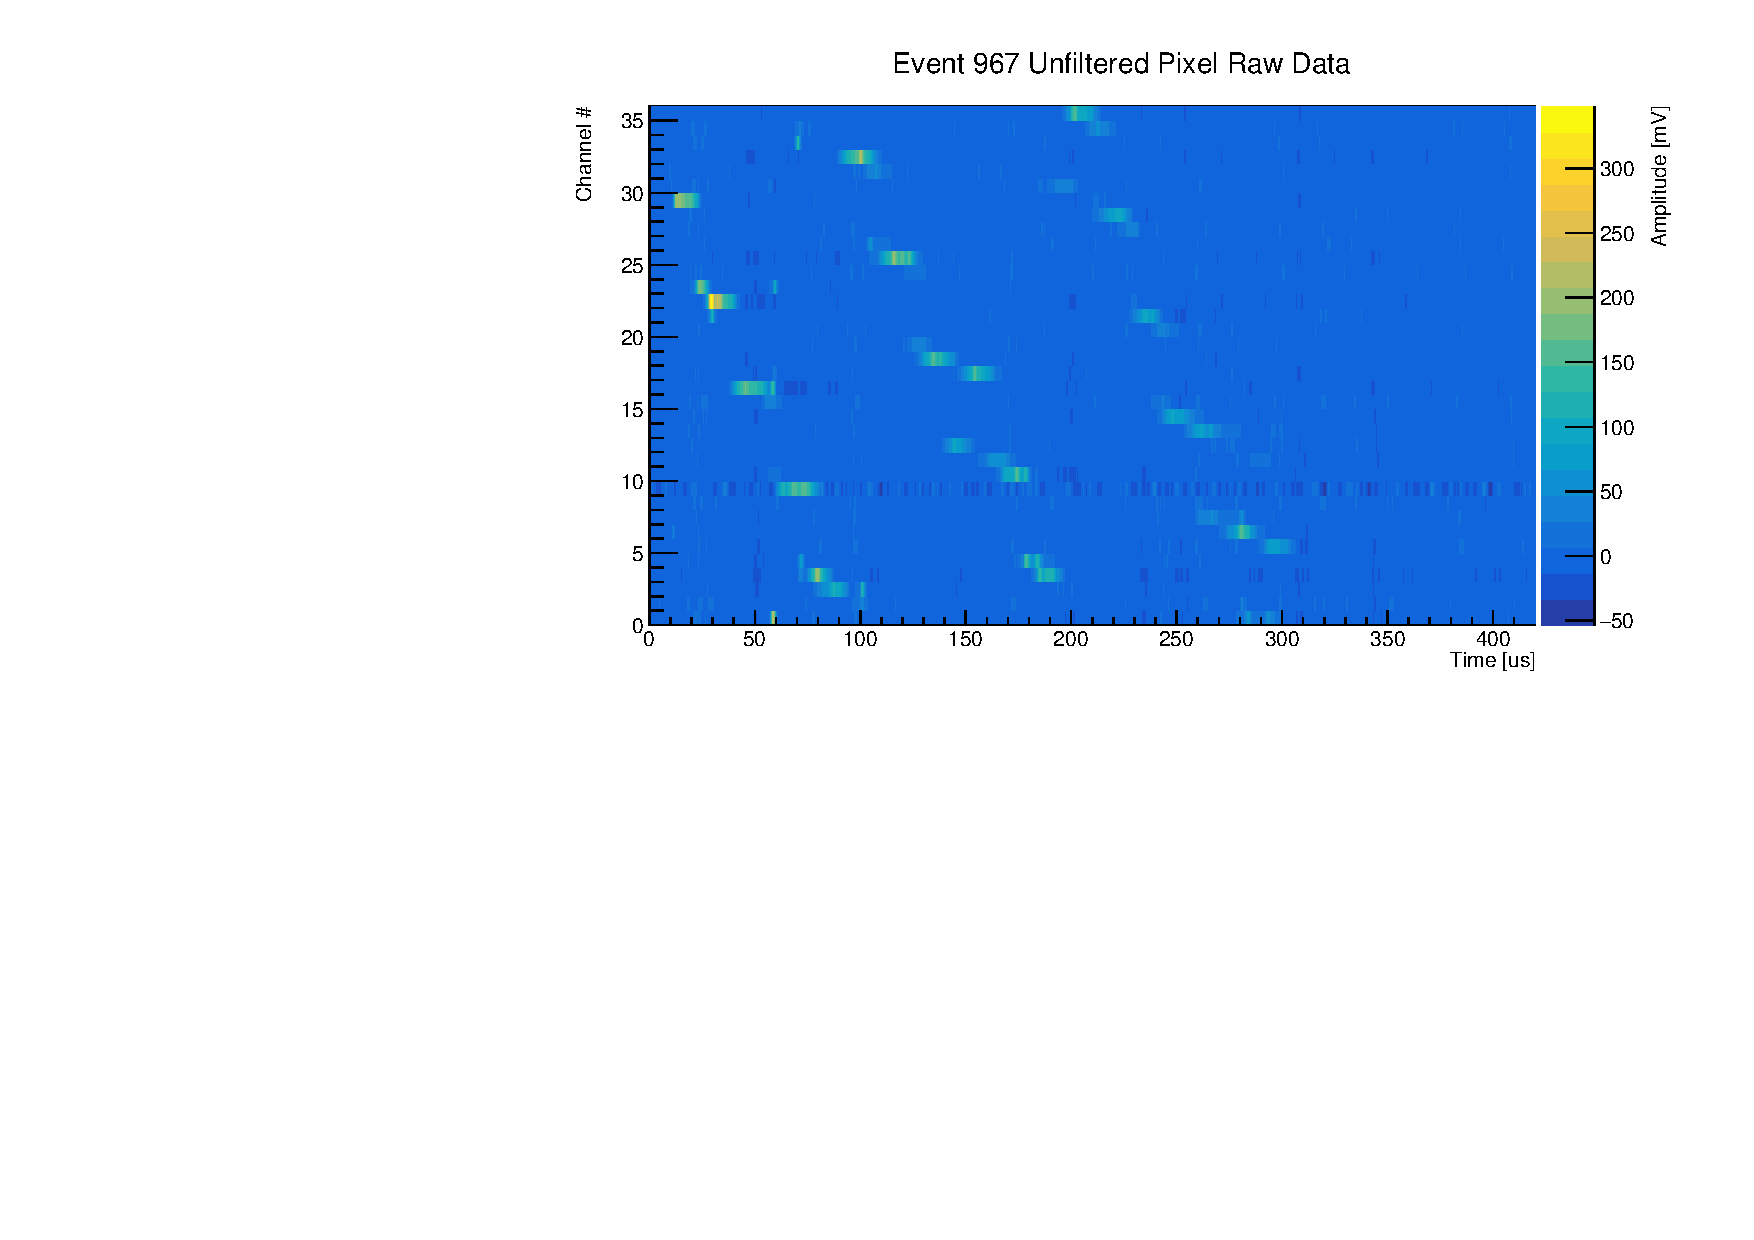
\includegraphics[width=\textwidth]{viper/event967_rawUnfilteredPixel}\\
	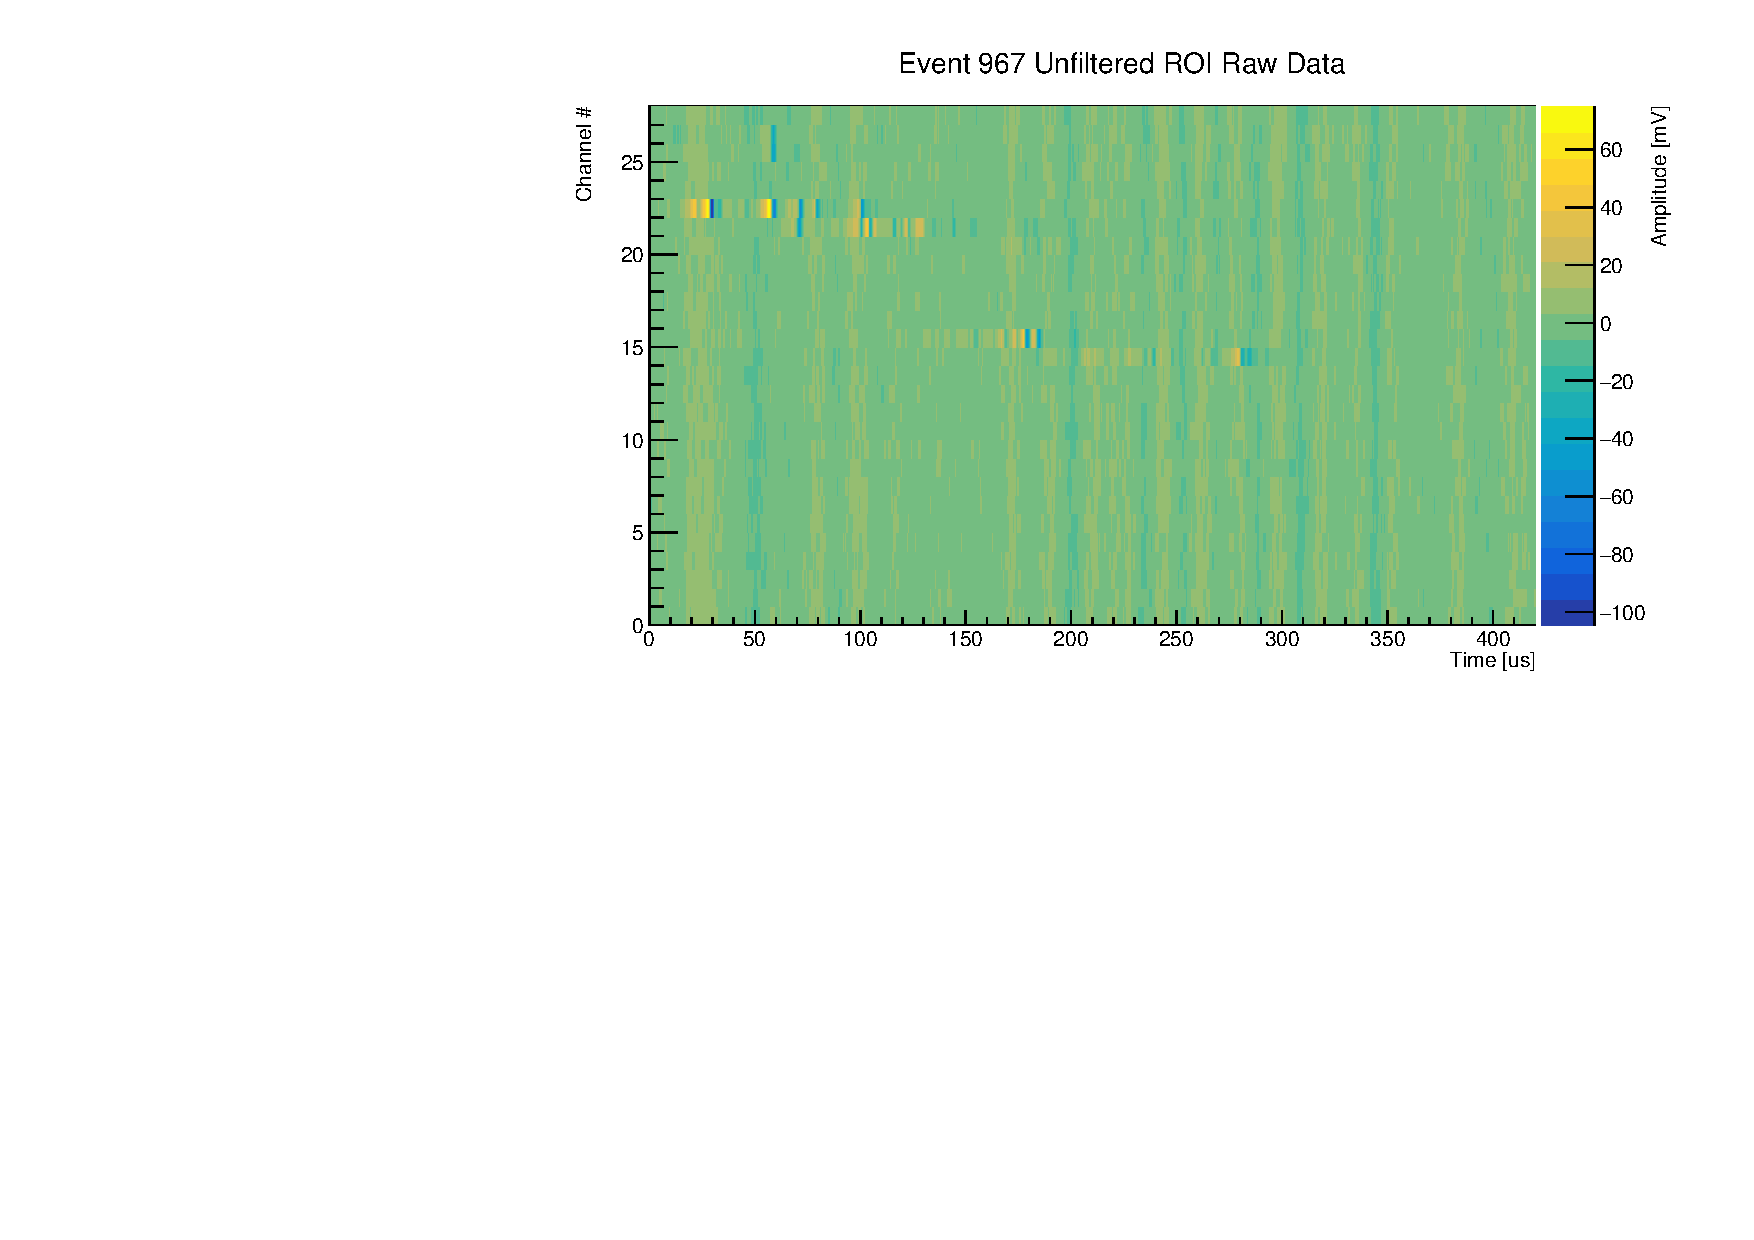
\includegraphics[width=\textwidth]{viper/event967_rawUnfilteredROI}
	\caption{Unfiltered raw data of a typical MIP event (the same event as in Figures~\ref{fig:viper_unfilteredRawData}~through~\ref{fig:viper_kalman}). The top plot shows pixel data while the bottom plot shows ROI data.}
	\label{fig:viper_unfilteredRawData}
\end{figure}

\begin{figure}[htb]
	\centering
	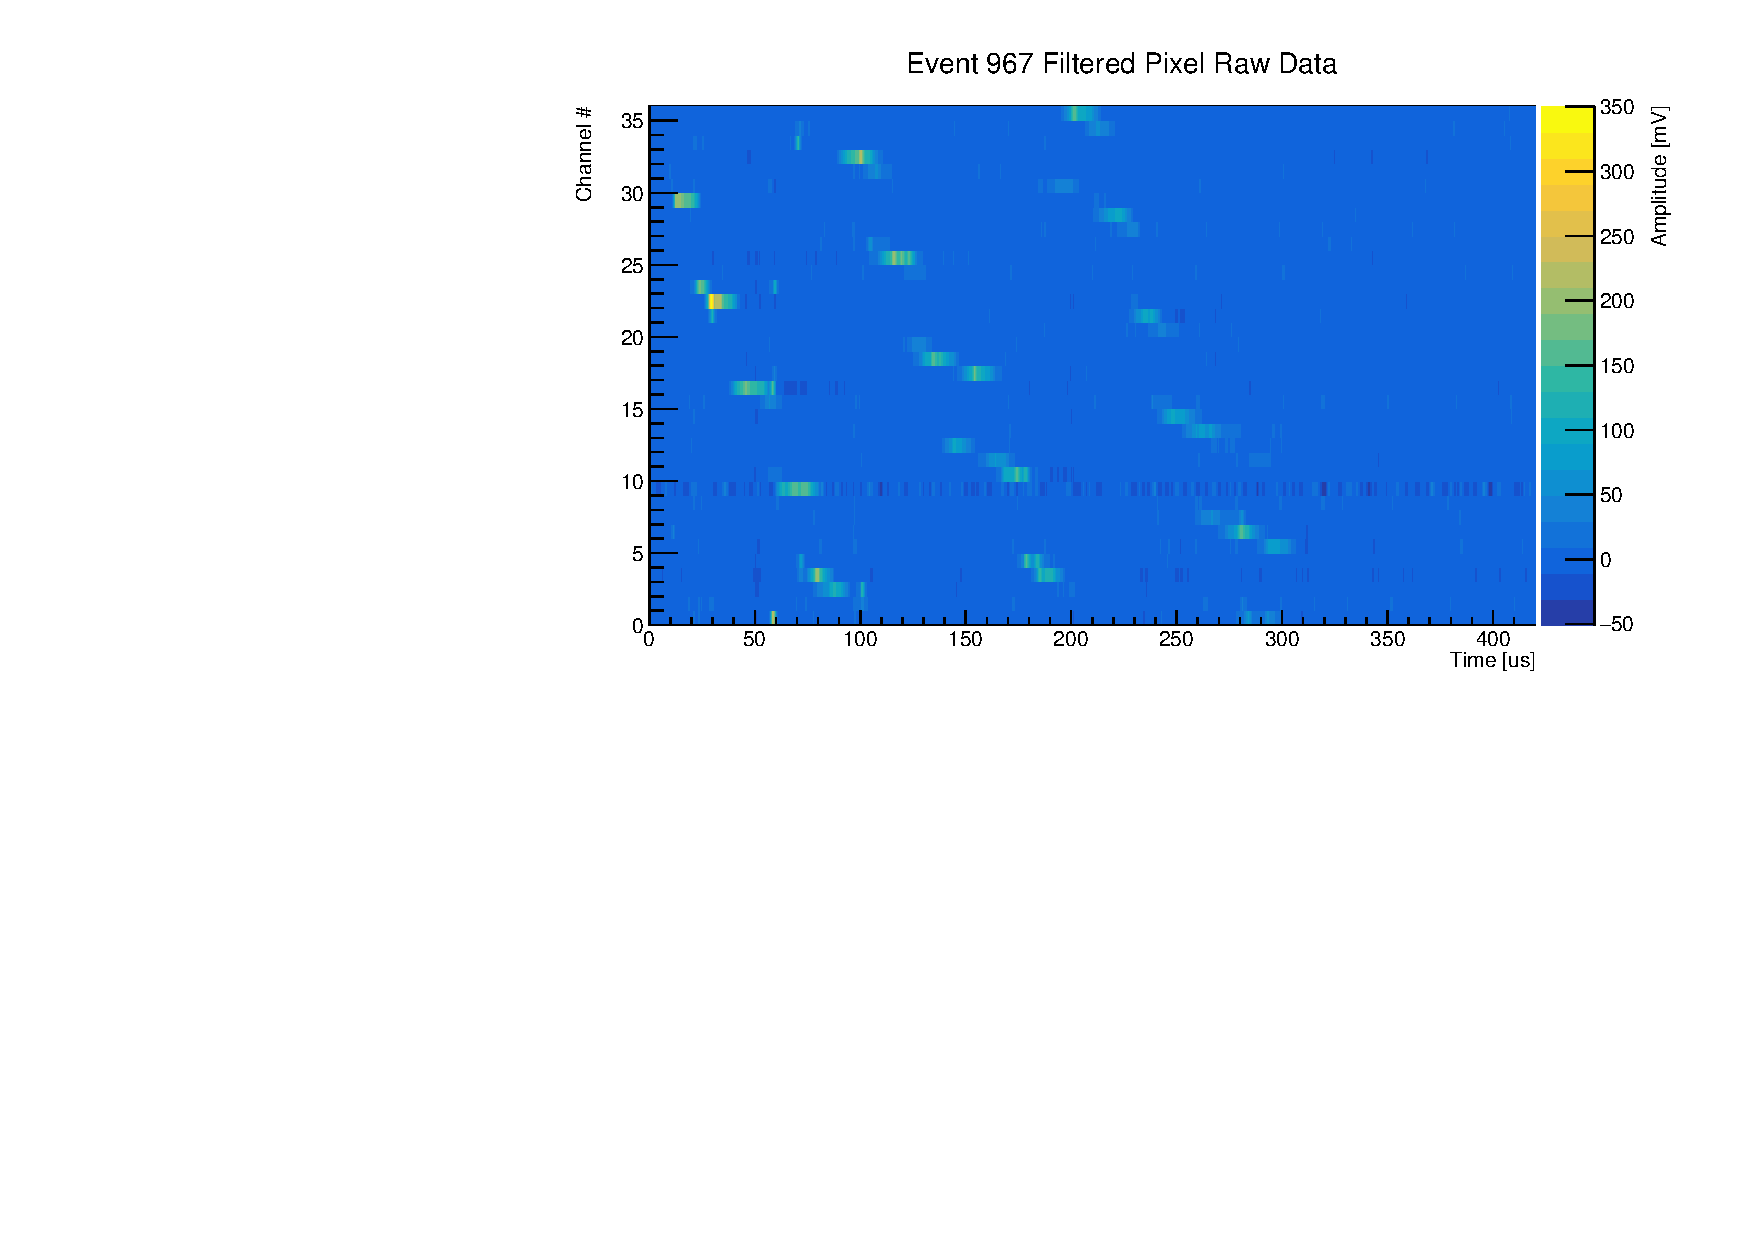
\includegraphics[width=\textwidth]{viper/event967_rawFilteredPixel}\\
	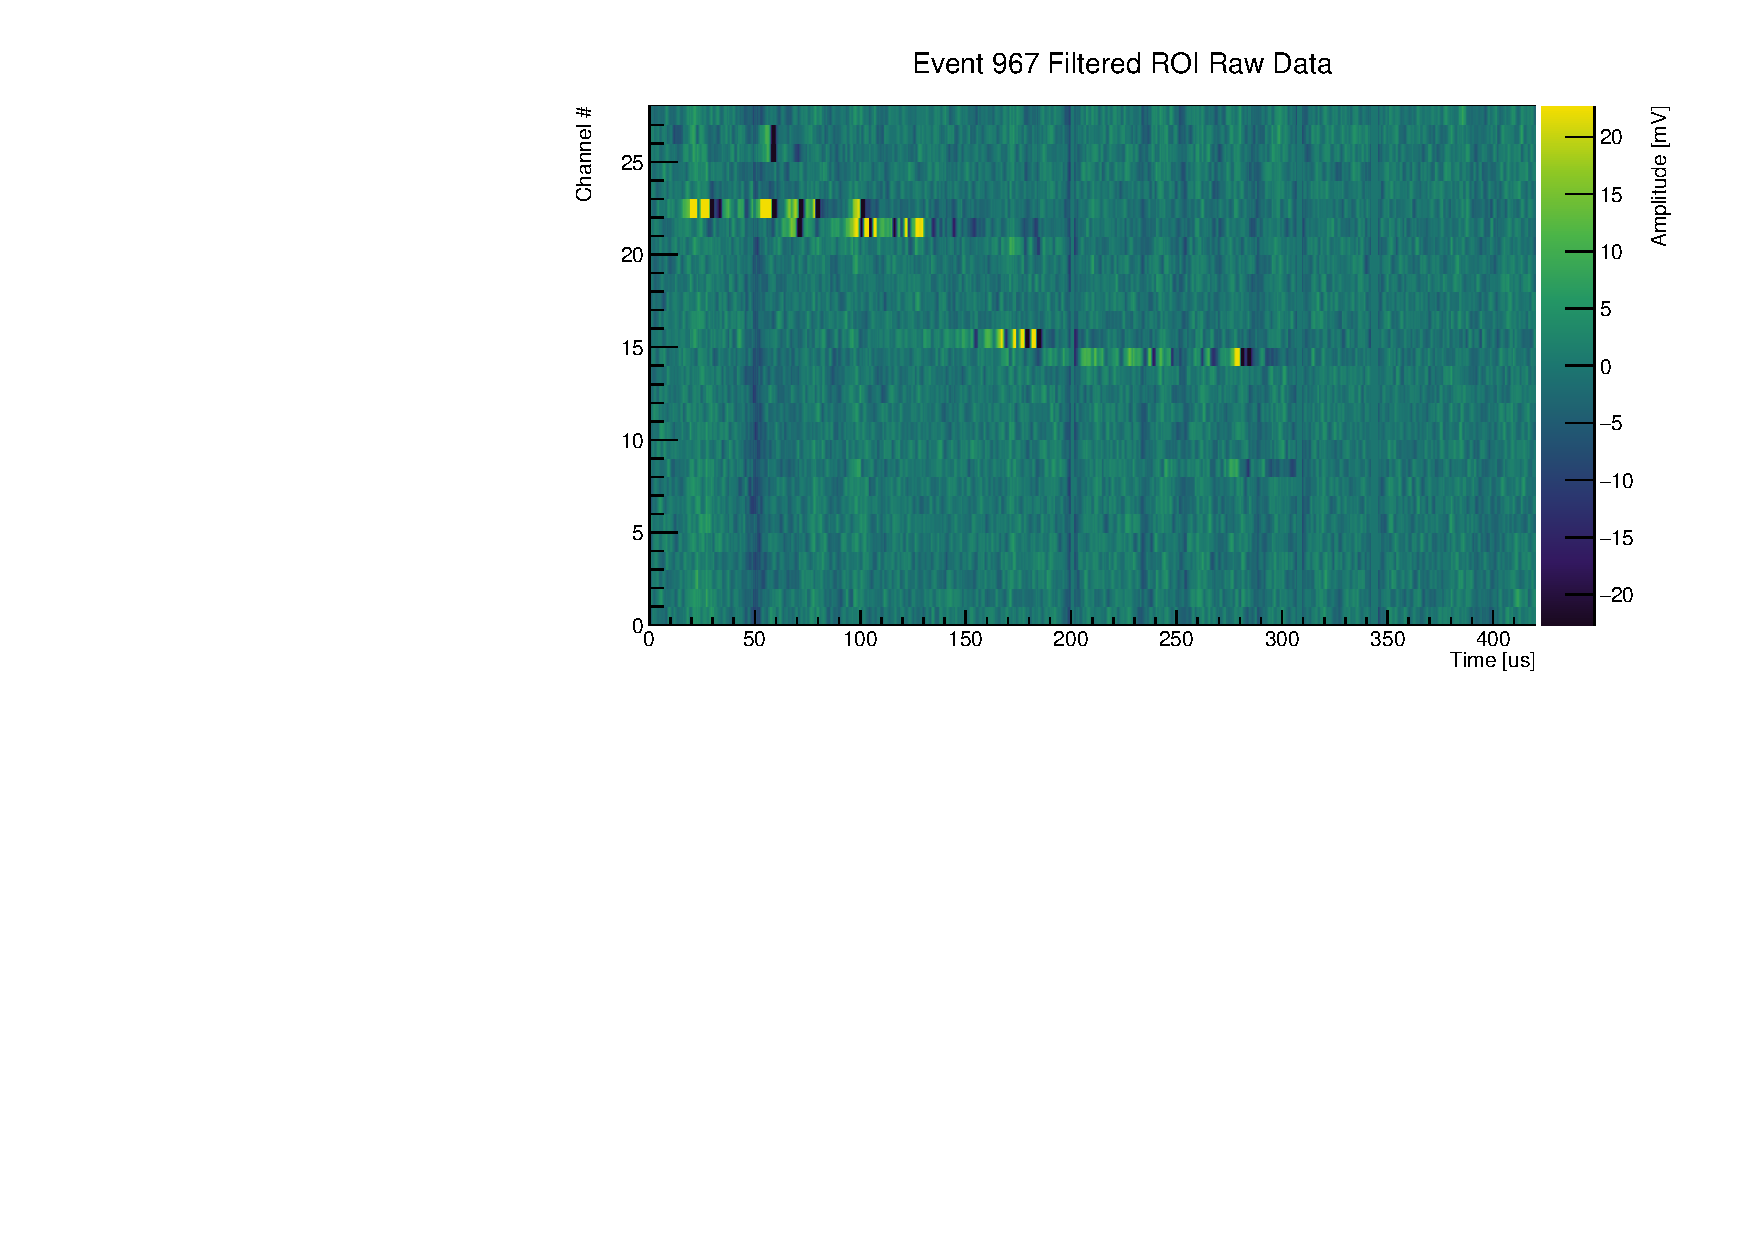
\includegraphics[width=\textwidth]{viper/event967_rawFilteredROI}
	\caption{Filtered data of a typical MIP event (the same event as in Figures~\ref{fig:viper_unfilteredRawData}~through~\ref{fig:viper_kalman}). The top plot shows pixel data while the bottom plot shows ROI data}
	\label{fig:viper_filteredRawData}
\end{figure}

The second step applies a recursive pulse finding algorithm.
The following is performed for each channel independently.
Most thresholds employed by the pulse finder are, again, defined in terms of noise amplitude.
Therefore, noise mean and standard deviation are recalculated after noise filtering.
A peak threshold is defined by multiplying the noise standard deviation by a variable scaling factor and adding the noise mean.
Then, the sample with the highest amplitude is found.
If it is below threshold, the process stops and proceeds to the next channel.
Otherwise, the pulse is scanned in positive and negative directions until it crosses respective lower noise thresholds.
After this, the whole pulse is deleted from the data and the process starts over with finding the new maximum sample and checking it against the peak threshold.
For stability reasons, the peak threshold relative to noise levels is compared against an absolute threshold and the higher of the two is applied.
The search is extended to the negative pulse for the bipolar ROI pulses.
The different thresholds employed and samples found by this process are illustrated in Figure~\ref{fig:viper_hitFinder}.

\begin{figure}[htb]
	\centering
	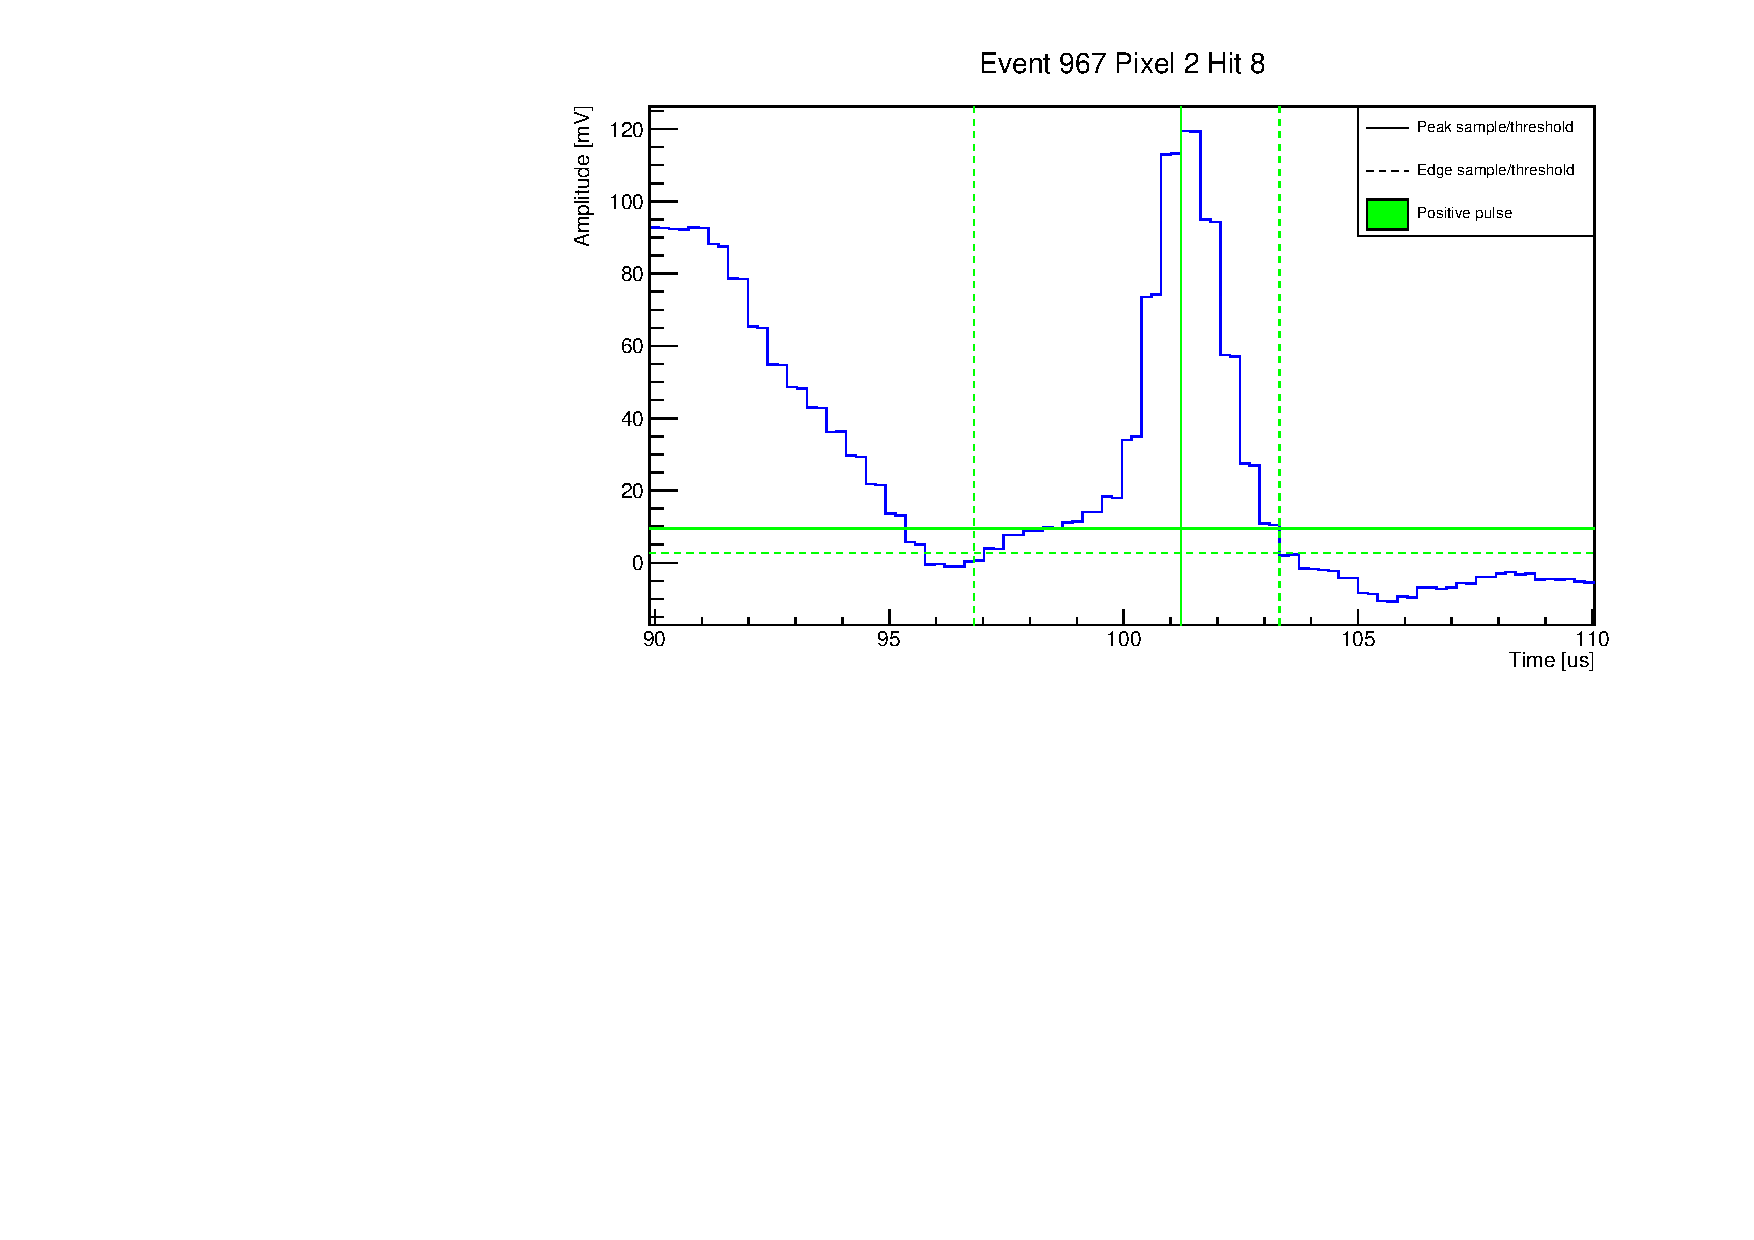
\includegraphics[width=\textwidth, page=1]{viper/event967_pixel2_hit8}\\
	\includegraphics[width=\textwidth, page=3]{viper/event967_pixel2_hit8}
	\caption{Pulse shapes of a single pixel (top) and ROI (bottom) hit of a typical MIP event (the same event as in Figures~\ref{fig:viper_unfilteredRawData}~through~\ref{fig:viper_kalman}).
	Superimposed are the thresholds of the hit finder algorithm. Horizontal lines represent thresholds: the solid is the minimum threshold required to be crossed for a pulse to be detected, and dashed are the thresholds used to detect the pulse edges.
	Vertical lines represent the corresponding detected peak/edge samples.
	Colour indicates a positive (green) or negative (red) pulse, or a zero crossing (yellow).}
	\label{fig:viper_hitFinder}
\end{figure}

Identified pulses are then combined into 3D hits by matching pixels pulses to ROI pulses.
For this proof of concept, this is done rather primitively by matching any pulses coinciding in time.
In Figure~\ref{fig:viper_hitFinder}, a pixel and ROI pulse are matched if their time slices, defined by the vertical dashed lines, overlap.
This third step results in a rather high amount of ambiguities but assures that no hits are missed.

To resolve the ambiguities, a Principal Component Analysis (PCA) is applied to the 3D space points in a fourth step.
This technique is well established and described in literature, e.g.~\cite{pca}.
Therefore, it shall be explained here only briefly.
The basic idea is to calculate three orthogonal eigenvectors of the 3D space point cloud.
A graphic interpretation of these eigenvectors are the three axis of an ellipsoid fitted to the data points.
In case the points form a track, one of these eigenvectors will have a much higher eigenvalue than the other two.
This eigenvector is taken as an estimate for the track direction.
The ambiguities can be resolved by selecting the one closest to the track estimate.
Furthermore, this procedure can be used to recursively reject outliers by forming a cylinder around the track estimate with a radius proportional to the second largest eigenvalue.
All hits outside this cylinder are rejected.
The procedure can be repeated by rerunning the PCA on the remaining points and performing another outlier rejection.
In a later stage of reconstructing more complex events, this algorithm can potentially be used to cluster 3D space points in order to separate multiple tracks.
The PCA ambiguity rejection is illustrated in Figure~\ref{fig:viper_pca}.

\begin{figure}[htb]
	\centering
	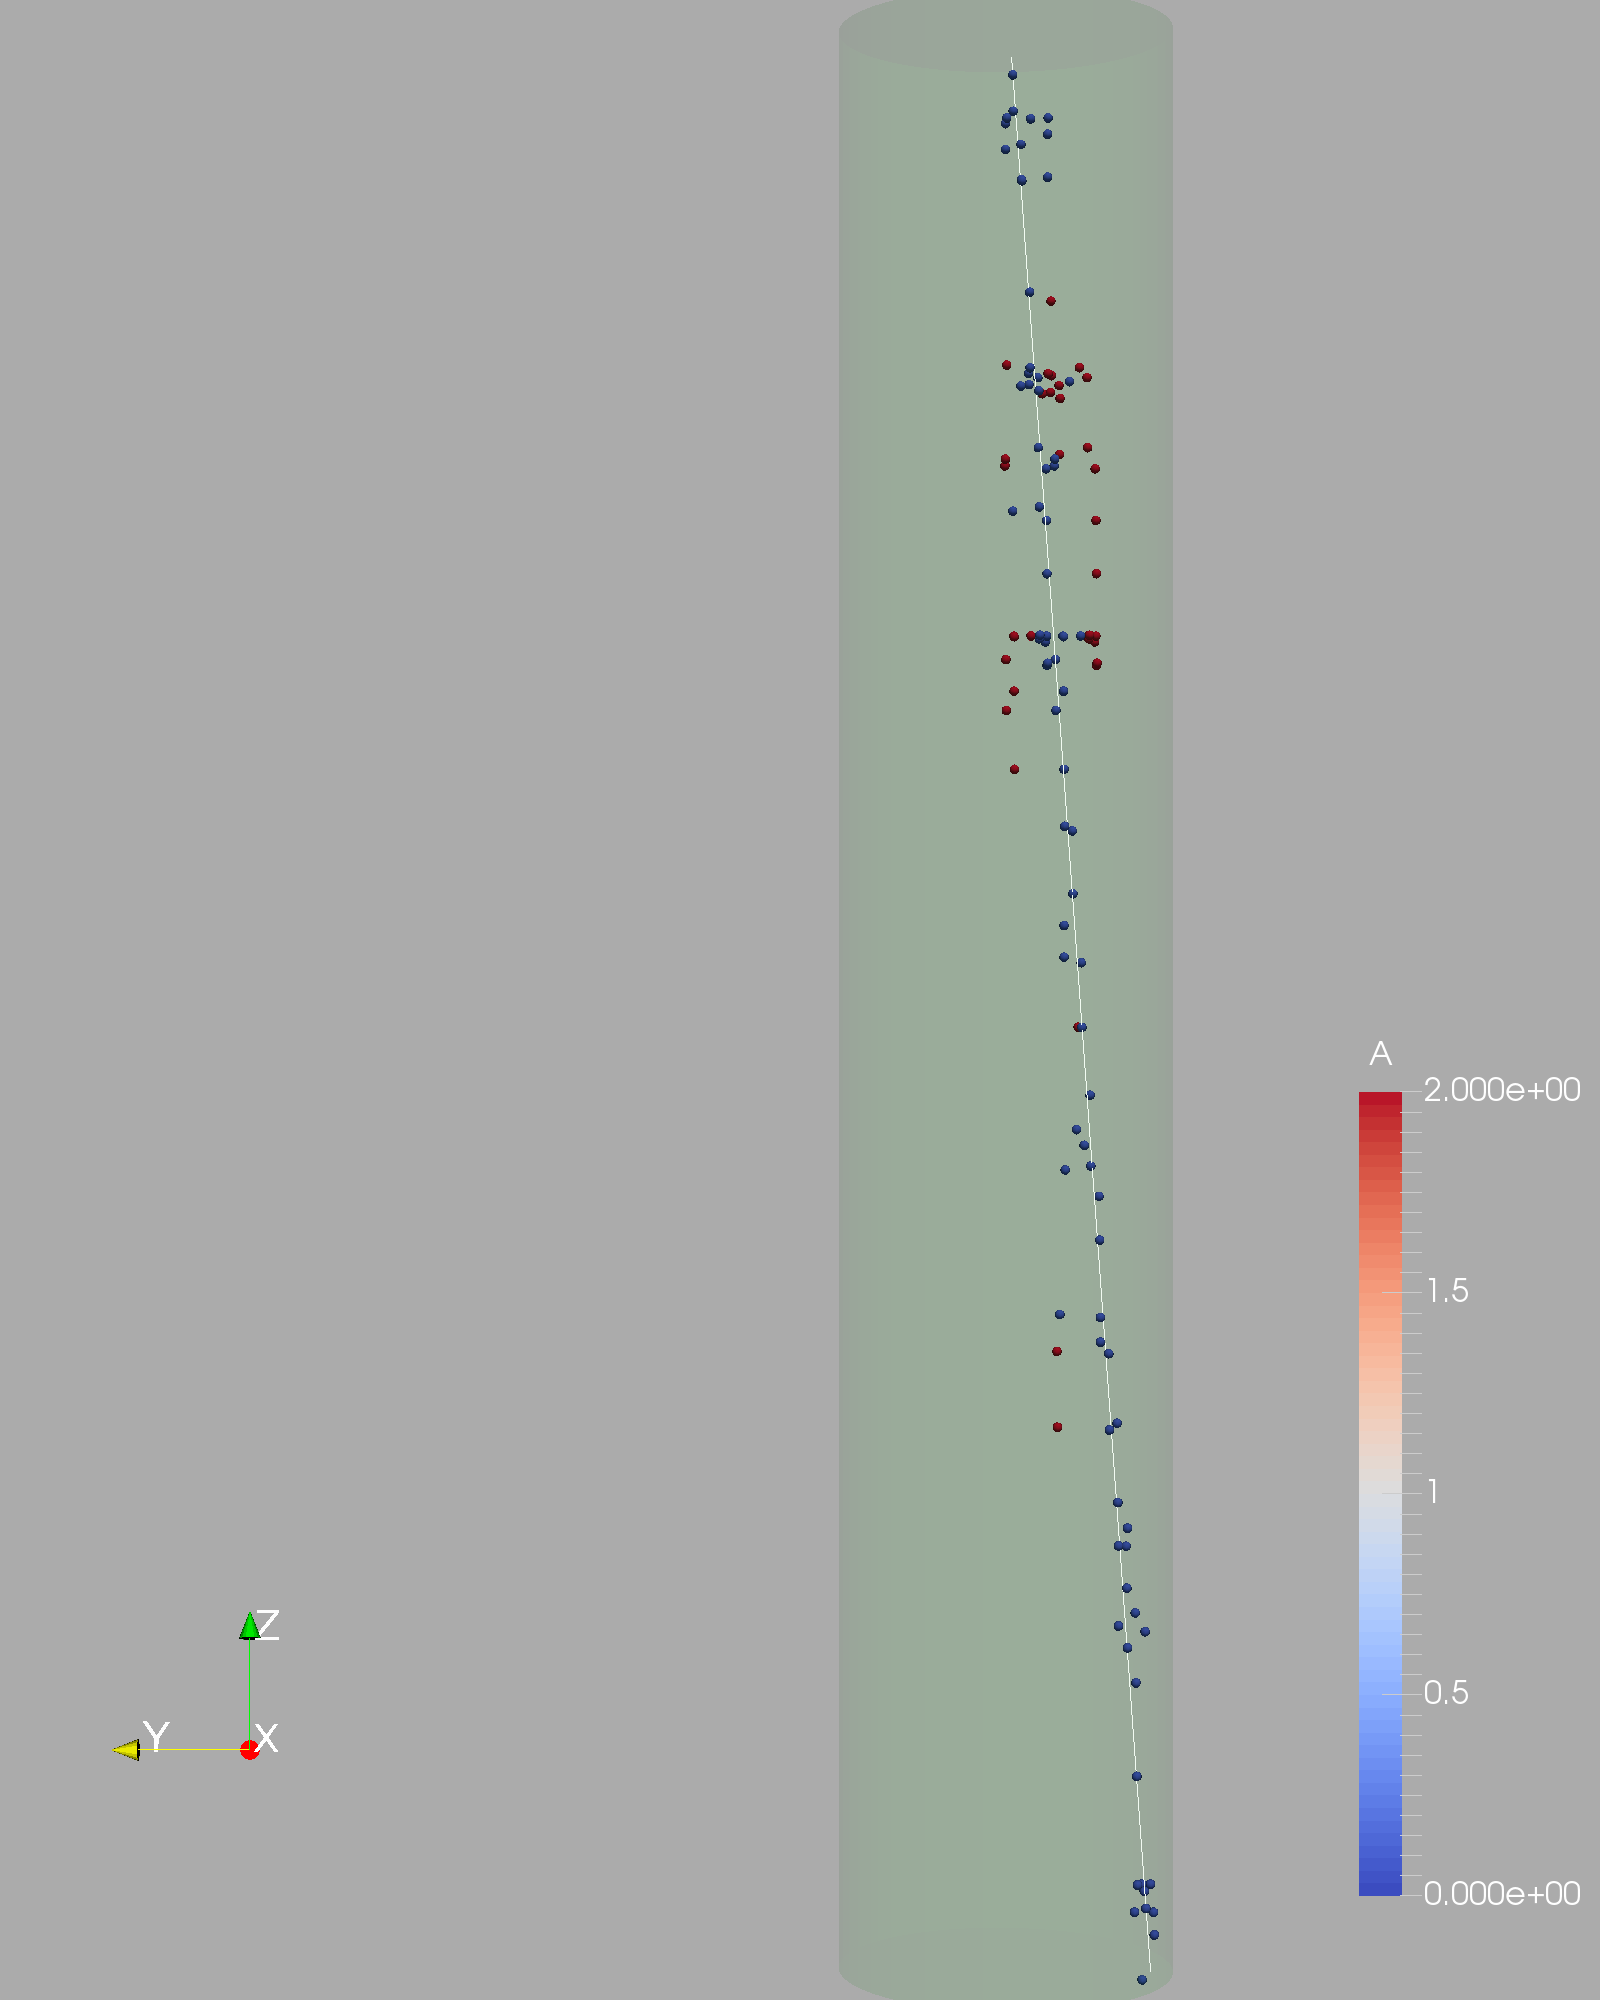
\includegraphics[viewport=800 0 1200 2000, clip, height=\textwidth, angle=90]{viper/event967_hits}
	\caption{Reconstructed 3D hits from the hit finder.
	The TPC volume is shown in faint green.
	The passing particle is most likely a cosmic $\mu$ entering from the left (the same event as in Figures~\ref{fig:viper_unfilteredRawData}~through~\ref{fig:viper_kalman}).
	Drift direction is from right to left.
	The colour of the hits indicates the result of the principal components analysis: blue is accepted as the true hit while rejected ambiguous hits are plotted in red.
	The thin white line represents the eigenvector with the largest eigenvalue of the ellipsoid formed by the 3D hit point cloud.
	As this is a quite clean track with only few short $\delta$ rays, there are no outliers rejected other than the multiplexing ambiguities.}
	\label{fig:viper_pca}
\end{figure}

The final step consists of a Kalman filter.
For this, the well-established GENFIT track fitting package~\cite{genfit1, genfit2} was used.
Ionisation losses and multiple scattering are taken into account.
The particle is assumed to be a minimum-ionising muon with an initial momentum of \SI{260}{\mega\electronvolt} in the direction of the track estimate from the PCA.
A recursive algorithm capable of dealing with outliers was chosen, a so-called \emph{deterministic annealing filter}.
This works by assigning successively lower weights to outliers with each recursion step.
For more details, see the respective publications~\cite{genfit1, genfit2}.
The resulting track is shown in Figure~\ref{fig:viper_kalman}.

\begin{figure}[htb]
	\centering
	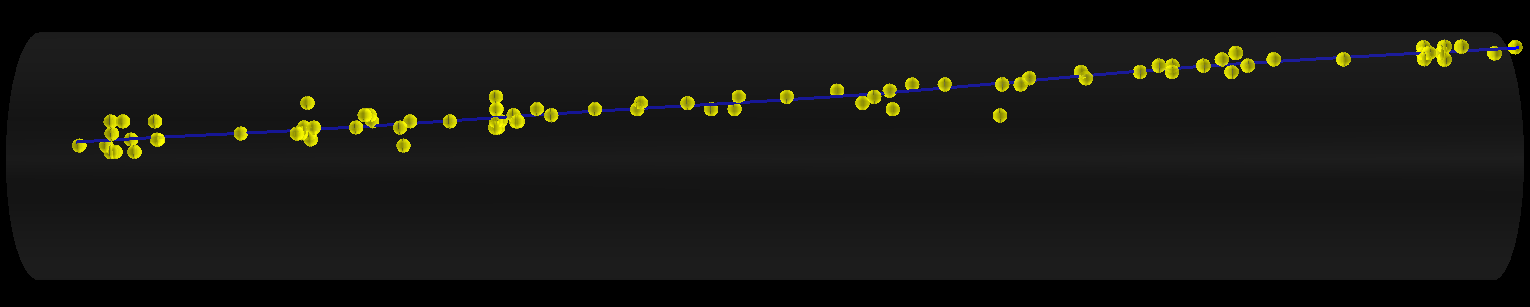
\includegraphics[width=\textwidth]{viper/event967_kalman}
	\caption{Track fitted by the Kalman filter.
	The TPC volume is shown in faint grey.
	The passing particle is most likely a cosmic $\mu$ entering from the left (the same event as in Figures~\ref{fig:viper_unfilteredRawData}~through~\ref{fig:viper_kalman}).
	Drift direction is from right to left.
	The yellow points are the input to the Kalman filter, the accepted hits from the principal components analysis.
	Blue is the output, a fitted track taking into account ionisation losses and multiple scattering in LAr.}
	\label{fig:viper_kalman}
\end{figure}

Technically, the Kalman filter would be capable of fitting the particle momentum or even particle type to the data.
At the time of this writing, this is not implemented yet.
In particular, the momentum stays roughly at the initial guess of \SI{260}{\mega\electronvolt}, assuming a minimum ionising muon in liquid argon.
A potential explanation for this is that the resolution of the detector is too low to estimate momentum from multiple scattering.
Another explanation might be the hit finder missing hits due to non-optimal tuning.
Proper tuning of the reconstruction requires a full simulation chain of the detector which is not yet available.
Using data to tune the reconstruction is prone to the introduction of circular biases.
On the other hand, most of the difficulties emerge from the multiplexing ambiguities and their resolution.
While the presented almost full 3D readout has already reduced the reconstruction complexity compared to a classical wire readout, an ambiguity-free readout will make reconstruction another big step easier by completely eliminating the need to resolve ambiguities.
\chapter{The \AC{} Approach}
\label{chap:argoncube}

To mitigate the drawbacks mentioned in Section~\ref{sec:lartpc_challenges}, the Bern group has founded the \AC{} collaboration, with the goal of developing a new fully-modular type of \lartpc{}.
Modularity reduces pile-up and allows for shorter drift-times, thus slackens the requirements on argon purity and HV.
A modular detector also contains light within each module, allowing for a more accurate trigger system.
Maintenance and upgrading of a modular detector is much easier than for a monolothic one.


\section{Modularity}
\label{sec:ac_modularity}

\AC{} is made of fully autarkic TPC modules.
In case of a fault condition the affected module(s) can be shut down and repaired or replaced individually without affecting the rest of the detector.
During construction, one can start data taking as soon as the first module is operational and needs not wait for the commissioning of the whole detector.
A modular detector furthermore reduces event pile-up because the acquisition time is reduced to the size of one module.
This is crucial in the high-multiplicity environments of future liquid argon neutrino detectors.
Finally, also trigger purity profits from a modular approach because scintillation light is contained within one module allowing for a localised trigger.

\begin{figure}[htb]
	\centering
	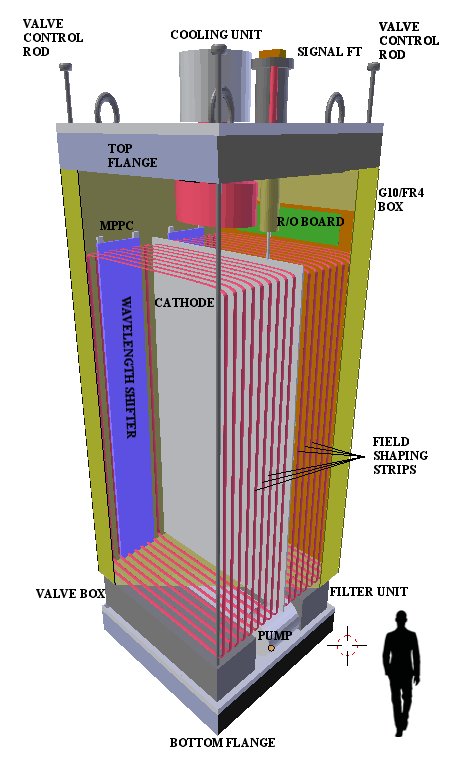
\includegraphics[height=.5\textheight]{ac/module}
	\caption{Schematic of an \AC{} module}
	\todo[inline]{better, more recent picture}
	\label{fig:ac_module}
\end{figure}

A module is made of a rectangular box with a square footprint and the height required by the detector design.
The top and bottom sides of the box are made from stainless steel while the sidewalls are made from FR-4.
FR-4 is a glass-reinforced epoxy composite widely used for printed circuit boards (PCBs).
The modules are placed side-by-side in a bath of liquid argon where they can be extracted and reinserted when needed.
Purity of the liquid argon is maintained within each module using an integrated recirculation system in the bottom of the module (see Section~\ref{sec:ac_cryo}).
As a result, the bath surrounding the modules needs not meet as stringent purity requirements as the argon inside.
Under normal operation conditions, all modules are inserted and the gaps between them are sealed off by indium seals pressed onto the top flanges.
The schematic of an \AC{} module is shown in Figure~\ref{fig:ac_module}.

To extract a module, the indium seal around the flange in question is removed and a drain pipe on the bottom of the module is opened.
The module is then slowly lifted up by a crane and the liquid argon is drained to the surrounding bath by means of gravity.
On the bottom of the module, a blind flange is located with equal dimensions as the top flange but without any feedthroughs.
When the bottom flange reaches the position of the top flange, it is sealed with indium again and then detached from the module which is now free and can be brought to its destination.
Upon reinsertion, the procedure is basically reversed.
First, the module is reattached to the blind flange and the indium seals is removed.
Then, the inner volume is opened to the surrounding bath to push the liquid argon into the module.
As opposed to extraction, the argon is guided through an oxygen trap as a first purification step.
The required pressure is supplied by the weight of the module floating on the liquid argon bath.
As soon as the top flange of the module reaches the top flanges of the other modules, the indium seal is reinstalled.
Figure~\ref{fig:ac_module-ins-ext} shows the insertion (left) and extraction (right) of a module.

\begin{figure}[htb]
	\centering
	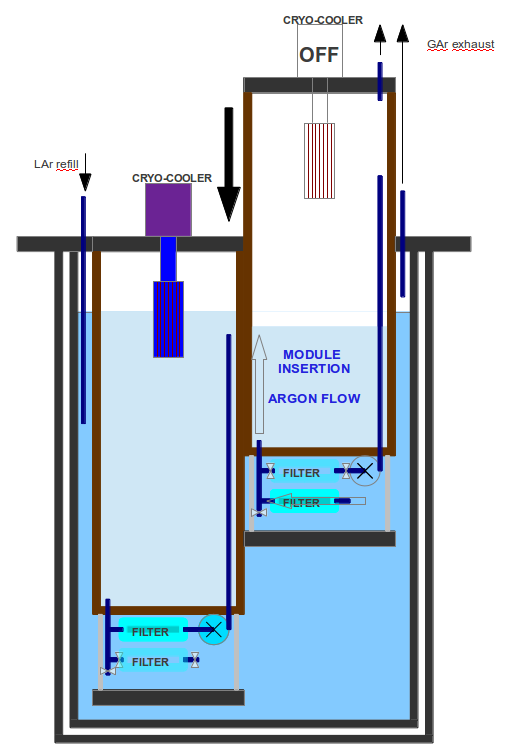
\includegraphics[width=.49\textwidth]{ac/module_insertion}
	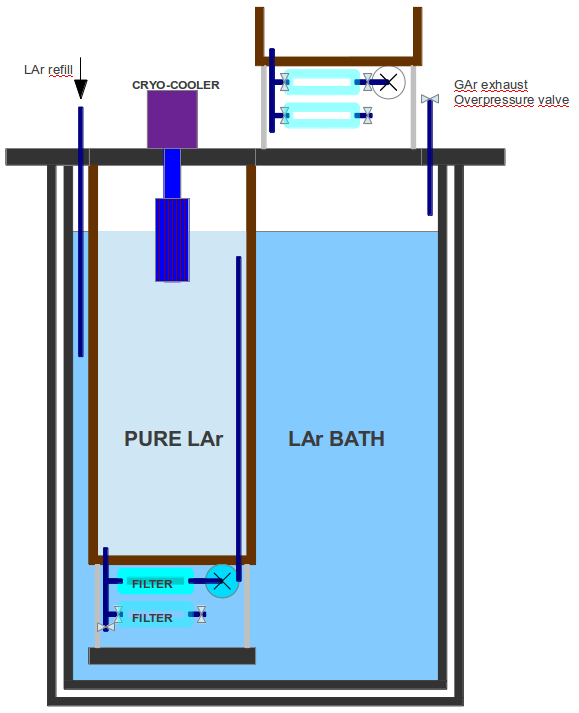
\includegraphics[width=.49\textwidth]{ac/module_extraction}
	\caption{Insertion (left) and extraction (right) of a module}
	\todo[inline]{better, more recent pictures?}
	\label{fig:ac_module-ins-ext}
\end{figure}

Another big problem that can be solved by a modular detector design are the high electric fields required for large detectors.
Because each module contains its own TPC independent of all other modules, the required cathode potential only depends on the module size not the detector size.
To minimise the cathode voltage, the field is applied along one of the short edges of a module and furthermore, the module is split in half by the cathode reducing the voltage by anoter factor of two.
Thus, for a module footprint of \SI{2 x 2}{\metre} and an electric field of \SI{1}{\kilo\volt\per\centi\metre}, a cathode potential of \SI{100}{\kilo\volt} is required.
Operating a \lartpc{} at this voltage is challenging but feasible without a prohibitive loss in fiducial volume~\cite{AT}.


\section{Cryogenics}
\label{sec:ac_cryo}


\section{Charge Readout}
\label{sec:ac_charge-readout}


\section{Light Readout}
\label{sec:ac_light-readout}
\chapter{Feasibility Study of a Pixelated LArTPC for the \dune Near Detector}
\label{chap:dune-nd}

With \AC\ selected as  the \lar\ component of the \dune\ near detector (ND), there were two main question that needed to be addressed:
\begin{enumerate}
	\item Is a pixelated \lartpc\ feasible?
	\item Can the \lar\ detector handle the high rates?
\end{enumerate}
Number one is addressed in Chapter~\ref{chap:viper}.
This chapter will address question number two.


\section{The High-Multiplicity Environment of the \dune\ Near Detector}
\label{sec:dune-nd_multiplicity}

One of the main goals of \dune\ is to measure the Dirac CP violation phase $\delta_{\m{CP}}$ provided it has a non-degenerate value.
To reach a $3 \sigma$ sensitivity for a \SI{75}{\percent} coverage of the $\delta_{\m{CP}}$ parameter space, an exposure of \SI{1320}{\kilo\tonne\mega\watt years} is required (see Figure~\ref{fig:dune-nd_cpv-sens}).~\cite{dune2}
Assuming the reference design of a \SI{40}{\kilo\tonne} far detector and a \SI{1}{\mega\watt} beam results in a data taking time of \SI{33}{years}.
Therefore, to make the data taking time shorter, a beam $> \SI{1}{\mega\watt}$ is required.
On the other hand, combining the numbers of the reference design in~\cite{dune2}, the event rate in the ND amounts to \SI{0.1}{evt\per\tonne\per\mega\watt} leading to significant event pile-up.
This number does not include rock events---secondary particles produced by beam neutrino interactions in the surrounding material, entering the detector.
The neutrino beam flux is depicted in Figure~\ref{fig:dune-nd_flux}.

\begin{figure}[htb]
	\centering
	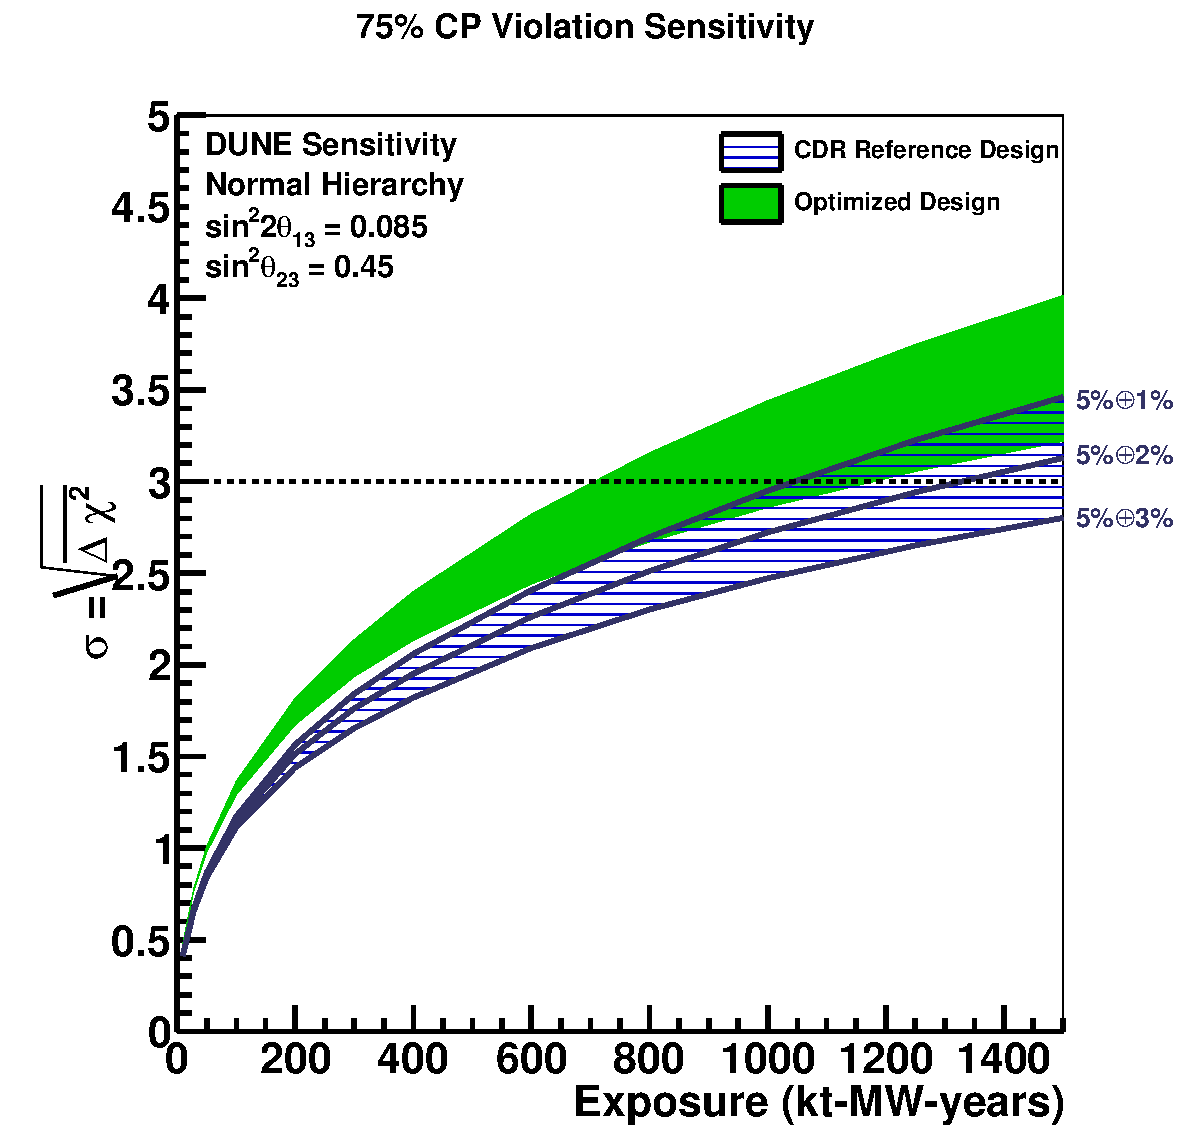
\includegraphics[width=.5\textwidth]{dune-nd/dune_cpv75_exp_syst}
	\caption{Expected sensitivity of \dune\ to discovery of CP violation, i.e.\ $\delta_{\m{CP}} \neq\ 0\ \m{or} \pi$ as a function of exposure in \si{\kilo\tonne\mega\watt years}, assuming equal running in neutrino and antineutrino mode.~\cite{dune2}}
	\label{fig:dune-nd_cpv-sens}
\end{figure}

\begin{figure}[htb]
	\centering
	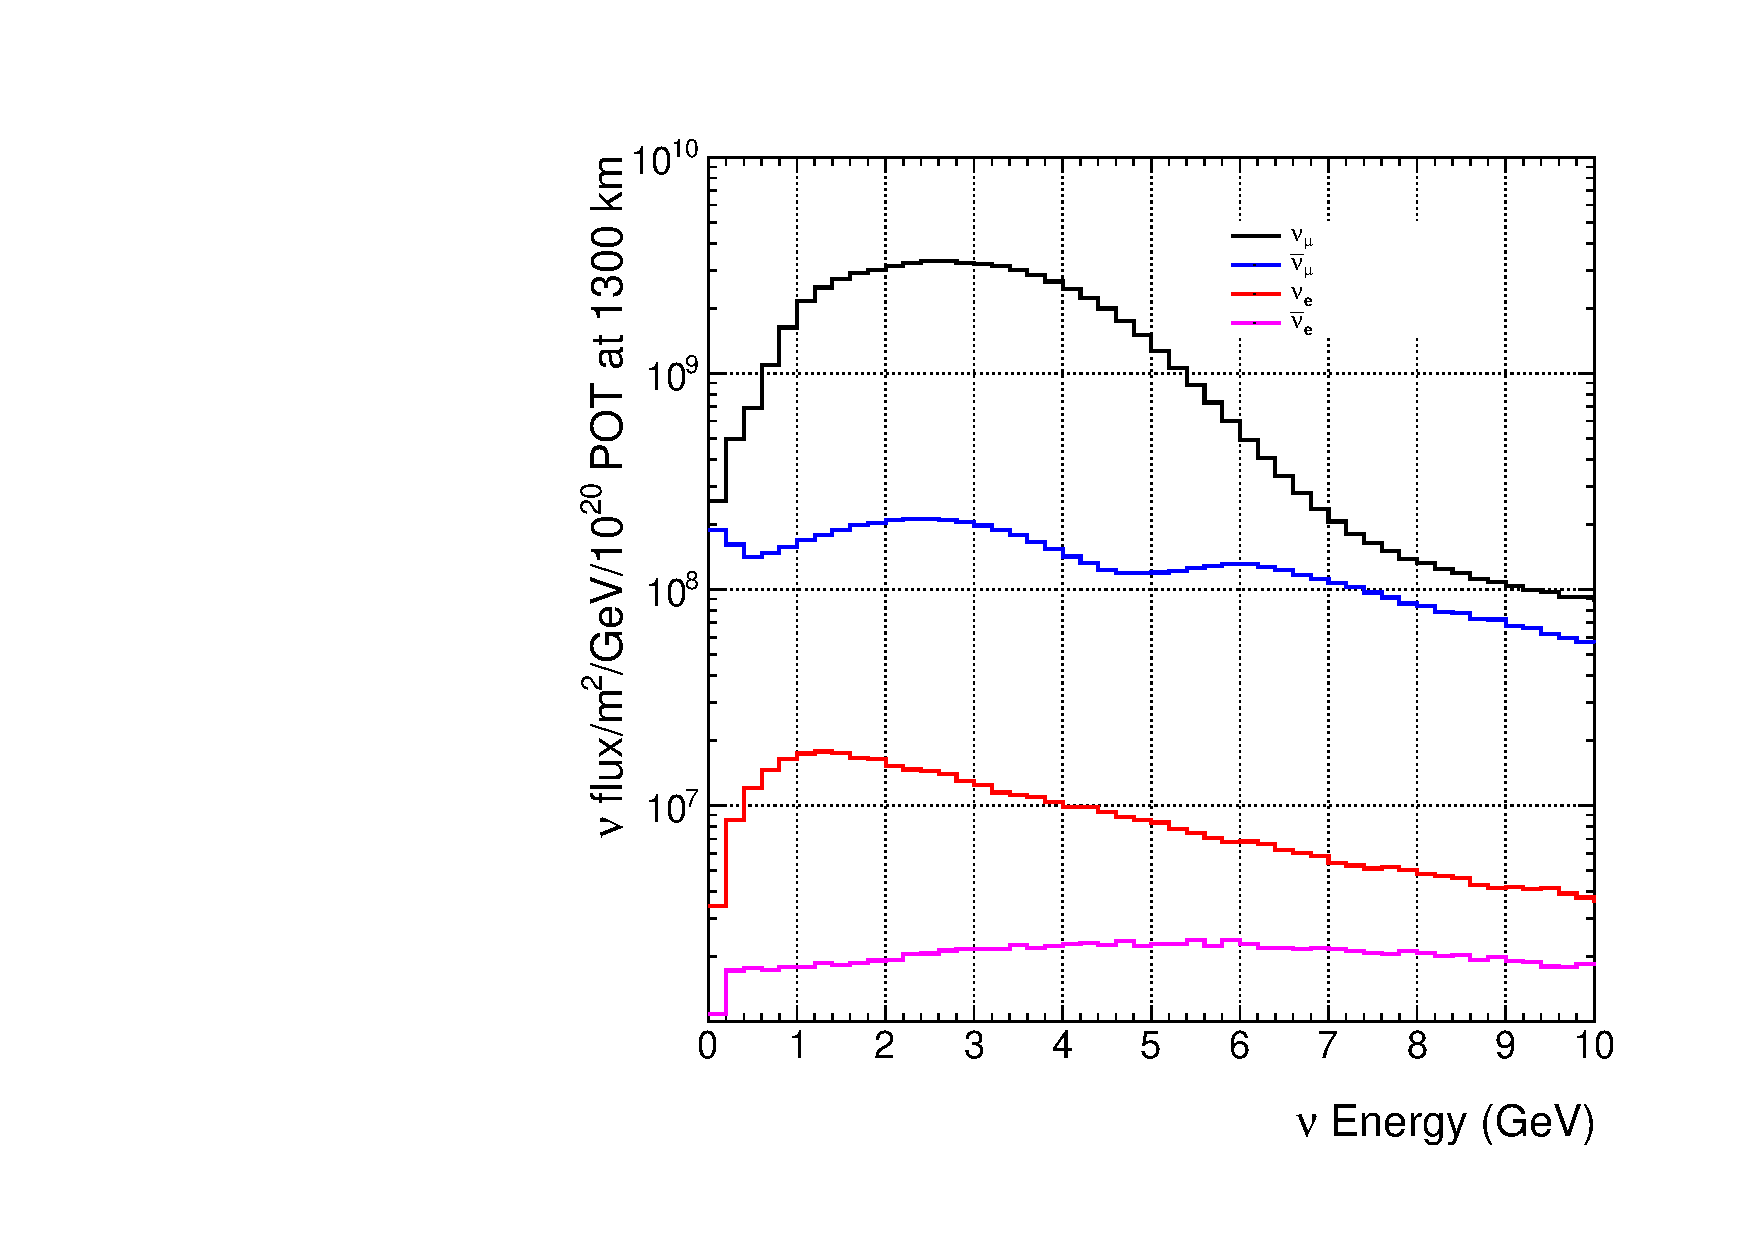
\includegraphics[width=.49\textwidth]{pile-up/FHC_230kA}
	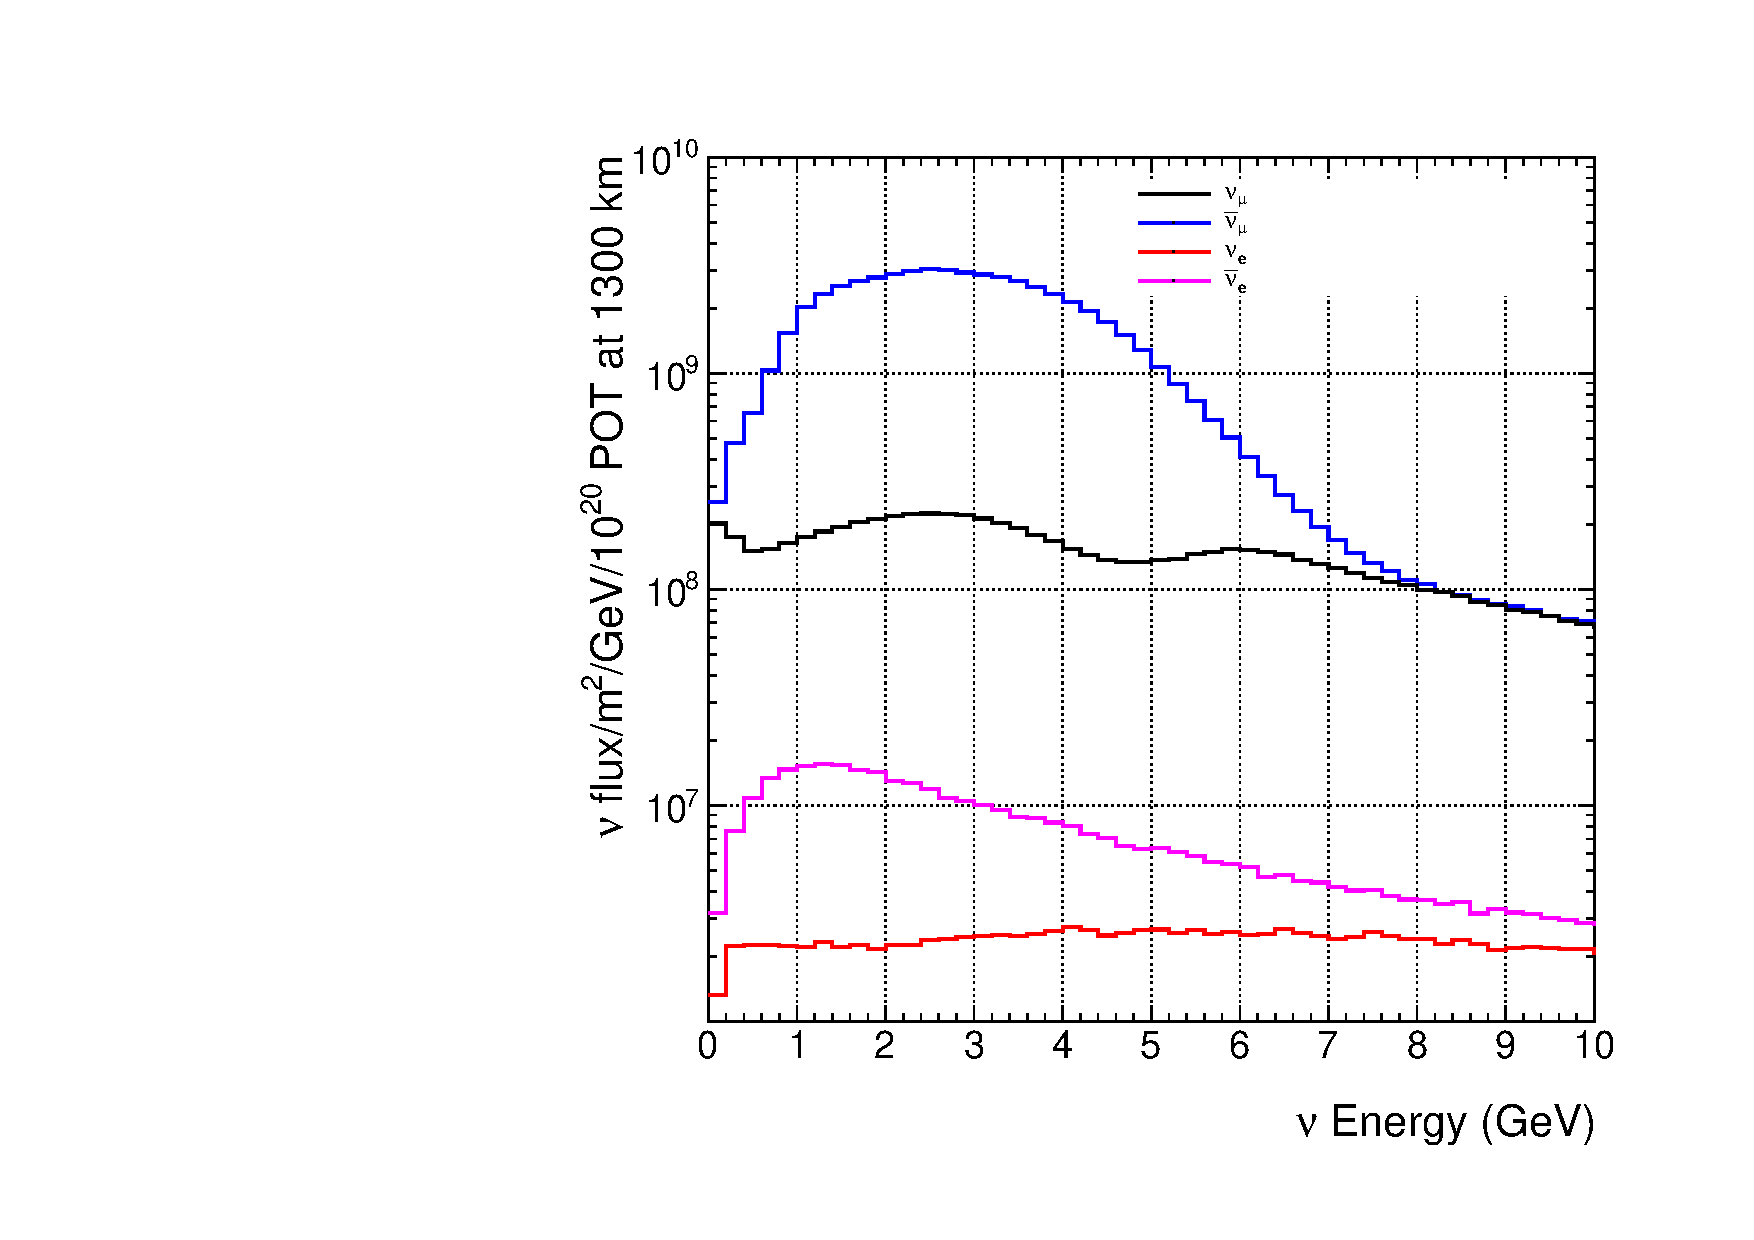
\includegraphics[width=.49\textwidth]{pile-up/RHC_230kA}
	\caption{Neutrino fluxes for the reference beam design operating in neutrino mode (left) and antineutrino mode (right), generated with a \SI{120}{\giga\electronvolt} primary proton beam.~\cite{dune2}}
	\label{fig:dune-nd_flux}
\end{figure}


\section{The Argon Box Simulation Tool}
\label{sec:dune-nd_argon-box}

Argon Box\footnote{\url{https://github.com/dadwyer/argon_box}} was developed with the goal of providing an easy-to-use simulation of particle interactions in \lar\ component of the ND.
At the time of this writing its feature set is quite limited, in particular it does not incorporate any other detector materials except for the box of argon.
Primary particles can either be provided by a particle gun (e.g.\ $e^-$, $n$, $p$, $\mu^+$) or in form of a \emph{HEPEVT} file---a file format standard for passage of particle events between different simulation tools.
For this study, several million neutrino events were produced with the GENIE\footnote{\url{https://genie.hepforge.org}} neutrino event generator.
Secondary particle transport and interaction in Argon Box is performed by Geant4.\footnote{\url{http://geant4.cern.ch}}
Finally, the energy deposition in \lar\ is voxelised and stored together with all the necessary ancillary information about the depositing particle.
The data is stored in the tree format of the ROOT data analysis framework.\footnote{\url{https://root.cern}}
This allows for convenient further processing using ROOT.


\section{$\pi^0$ pile-up study}
\label{sec:dune-nd_pile-up}

A significant amount of $\pi^0$ are produced in several resonant and coherent neutrino interactions (see Section~\ref{sec:nu-detection_interactions} and~\cite{dune2}).
They decay according to
\begin{IEEEeqnarray}{rCl}
	\pi^0 & \qraq & \gamma + \gamma
\end{IEEEeqnarray}
with a branching ratio of \SI{98.8}{\percent}\cite{pdg}.
The photons subsequently produce electromagnetic showers in \lar\ (see Section~\ref{sec:nu-detection_fs}).
At the energies of the \dune\ beam (see Figure~\ref{fig:dune-nd_flux}), most showers do not deposit a homogenous cone of charge but rather a lot of individually resolvable $e^{\pm}$ tracks.
More importantly, there often are significatn gaps in betweend these charge clusters.
A main challenge of shower reconstruction is to associate these well separated charge blobs to the correct event.
Misidentiions lead to a misreconstruction of the neutrino energy.
The resulting discrepancy to the true neutrino energy has the potential to skew the measured energy spectrum and, thus, influence the oscillation measurements.
The complexity of reconstruction paired with the potential impact on the physics measurements makes photons produced by $\pi^0$ decays a good sample to study the robustness to pile-up of a pixelated \lartpc\ in the \dune\ ND environment.

\begin{table}[htb]
	\centering
	\caption{Parameters of the $\pi^0$ pile-up simulation.}
	\label{tab:dune-nd_pile-up-params}
	\begin{tabu} to \textwidth {|l|S|}
		\hline
		{Beam direction} &			{$Z$ (positive)} \\
		\hline
		{Gravitation} &				{$Y$ (negative)} \\
		\hline
		{Resolution $X$} &			\SI{3}{\milli\metre} \\
		\hline
		{Resolution $Y$} &			\SI{3}{\milli\metre} \\
		\hline
		{Resolution $Z$} &			\SI{3}{\milli\metre} \\
		\hline
		{Target volume $X$} &		\SIrange{-1000}{5000}{\milli\metre} \\
		\hline
		{Active volume $X$} &		\SIrange{0}{4000}{\milli\metre} \\
		\hline
		{Fiducial volume $X$} &		\SIrange{300}{3700}{\milli\metre} \\
		\hline
		{Target volume $Y$} &		\SIrange{-1000}{3500}{\milli\metre} \\
		\hline
		{Active volume $Y$} &		\SIrange{0}{2500}{\milli\metre} \\
		\hline
		{Fiducial volume $Y$} &		\SIrange{300}{2200}{\milli\metre} \\
		\hline
		{Target volume $Z$} &		\SIrange{-4000}{5000}{\milli\metre} \\
		\hline
		{Active volume $Z$} &		\SIrange{0}{5000}{\milli\metre} \\
		\hline
		{Fiducial volume $Z$} &		\SIrange{300}{4700}{\milli\metre} \\
		\hline
		{Detection threshold} &		\SI{0.1}{\mega\electronvolt} \\
		\hline
		{Cone extent} &				{$10 X_{\m{0}} = \SI{1400}{\milli\metre}$} \\
		\hline
		{Cone half opening angle} &	\SI{15}{\degree} \\
		\hline
		{Cylinder radius} &			\SI{25}{\milli\metre} \\
		\hline
		{Beam intensity} &			{$\SI{2}{\mega\watt} \widehat{=} \SI{0.2}{evt\per\tonne}$} \\
		\hline
	\end{tabu}
\end{table}

To investigate the effects of pile-up on energy reconstruction, a working reconstruction algorithm is necessary.
However, at the time of writing, official reconstruction tools were only available for \lartpc s read out by wire planes.\footnote{\url{http://larsoft.org}}
Therefore, a rather primitive algorithm for true 3D space points was implemented, under the assumption that a positive outcome of such a pile-up study would imply an even better performance of a more sophisticated reconstruction.
This algorithm is explained in the following.
All its parameters are listed in Table~\ref{tab:dune-nd_pile-up-params}.

\begin{figure}[htb]
	\centering
	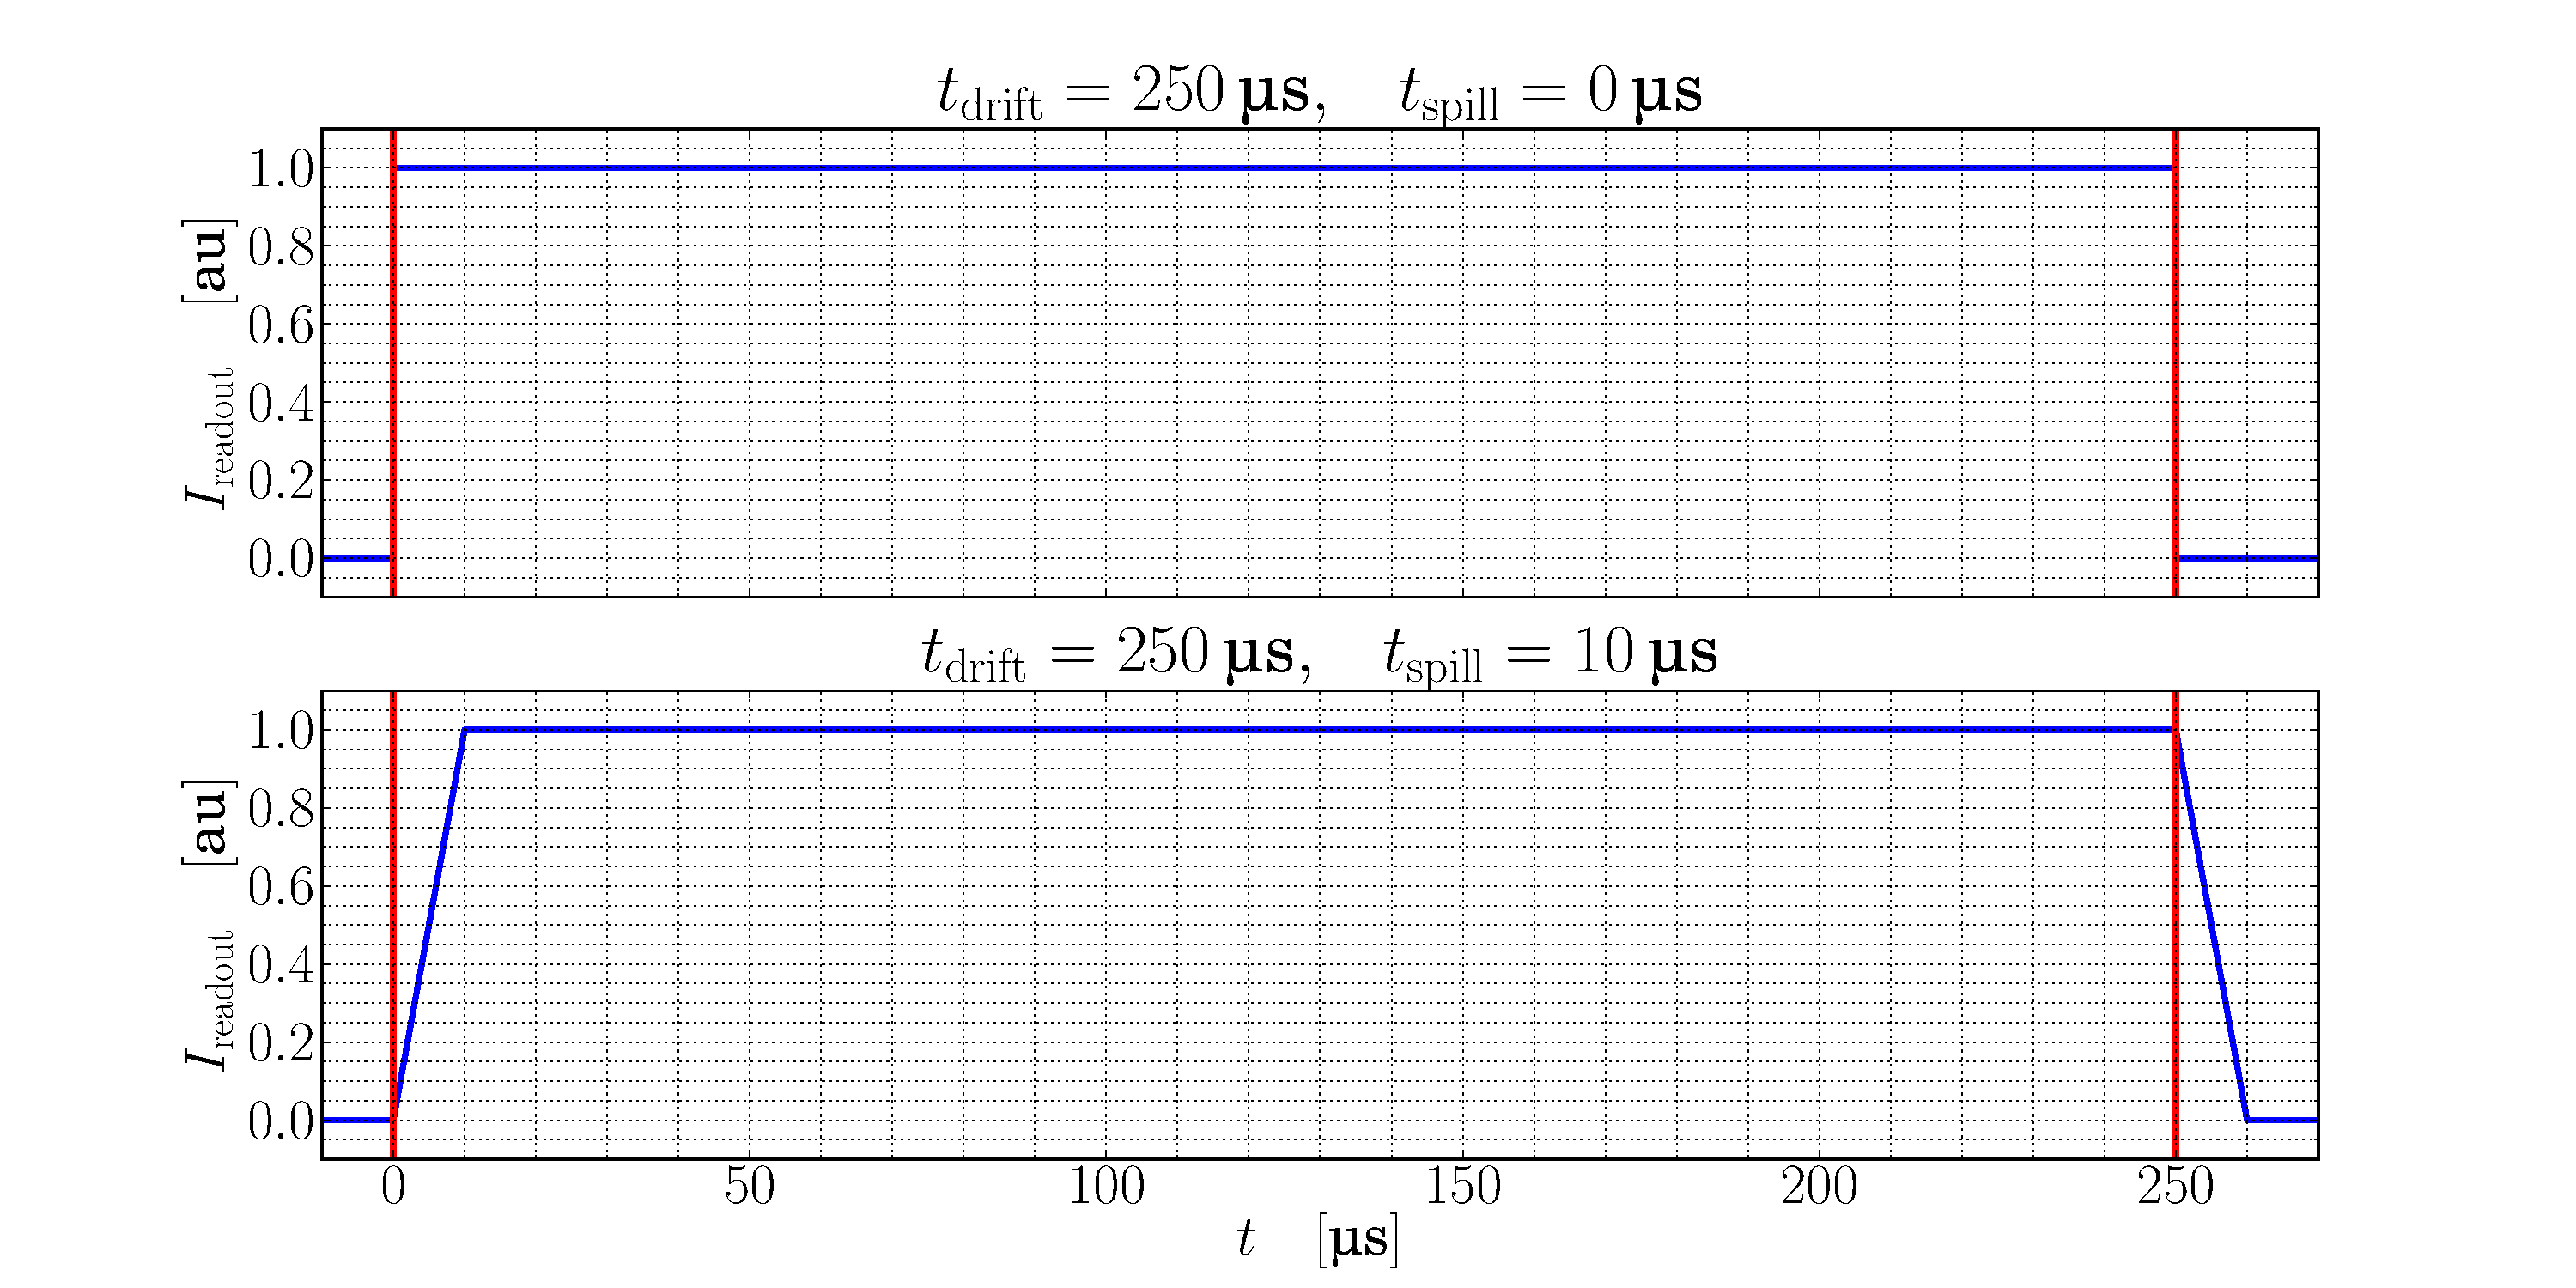
\includegraphics[width=\textwidth]{pile-up/charge_flux}
	\caption{Average current collected by the readout for one spill as a function of time.
	The current is given in arbitrary but equal units for both plots.
	The upper plot assumes the whole charge is deposited instantaneously while for the lower plot, the actual spill duration from~\cite{dune2} is used.}
	\label{fig:dune-nd_charge-flux}
\end{figure}

The basic underlying assumption is that a non-multiplexed pixel readout will yield unambiguous 3D space points of charge deposition with a given resolution, depending on the geometry of the pixel plane, time resolution of the readout electronics, and charge transport effects.
Furthermore, it is assumed that EM shower can be identified and their starting point and direction reconstructed with negligible errors and inefficiencies, i.e.\ this information is taken from the simulation truth.
A cone is calculated in the direction of the shower with its tip at the first charge deposition of the initial photon.
The opening angle and longituginal extent of the cone were optimised by looking at the distributions of the distance from the starting point and angle w.r.t. the direction of the shower.
The finite resolution of the detector is emulated by voxelising the charge deposition with the corresponding resolution in all three spatial coordinates.
This leads to problems near the tip of the cone where the transversal extent is lower than the voxel dimensions.
In particular, it can happen that most of the initial charge is shifted outside the cone.
Furthermore, multiple scattering at lower energies makes the cone model suboptimal near the tip.
Therefore, the acceptance volume for the reconstruction is taken as the union of the cone with a cylinder around the direction of the shower of the same longitudinal extent as the cone.

\begin{figure}[htb]
	\centering
	\includegraphics[width=\textwidth]{pile-up/2MW/eff_pur}
	\caption{Efficiency (accepted true over total true energy deposition) and purity (accepted true over total accepted energy deposition) distributions of a simple cone-cylinder union EM shower reconstruction algorithm.
	The distribution represents the fraction of photons produced by $\pi^0$ whose energy was reconstructed with the corresponding efficiency/purity.
	Purity is shown for four different selections of misidentified energy: total (magenta); deposited by other events only (cyan); deposited by other events only, excluding muons (red), deposited by photons and neutrons from other events only (blue).
	The simulated beam intensity is \SI{2}{\mega\watt}.}
	\label{fig:dune-nd_2MW-eff-pur}
\end{figure}

Argon Box propagates the neutrino interaction events it gets from GENIE through liquid argon, the output is a ROOT tree of neutrino interaction events.
To get a realisitc simulation of beam events in the detector, these events need to be distributed randomly in time and space.
Beam spills are simulated by drawing the number of events for each spill from a Poisson distrubition whose mean is calculated from the beam intensity and the target mass.
The resulting number of events is taken from the Argon Box ROOT tree and their vertices are placed within the \lar\ volume at coordinates drawn from a uniform distribution.

\begin{figure}[htb]
	\centering
	\includegraphics[width=\textwidth]{pile-up/2MW/energy_error}
	\caption{Fractional error on the reconstructed neutrino energy due to missed or misidentified energy depositions as a function of true neutrino energy.
	Misidentified energy is shown for three different selections: total deposited by other events (cyan); deposited by other events excluding muons (red), deposited by photons and neutrons from other events only (blue).
	The simulated beam intensity is \SI{2}{\mega\watt}.}
	\label{fig:dune-nd_2MW-energy-error}
\end{figure}

Three different argon volumes are assumed for the simulation: target, active, and fiducial volume.
The actual detector dimensions are represented by the active volume.
It is inside the target volume which is the volume within which the neutrino vertices are placed randomly.
This is done as a crude emulation of rock events, secondary particles from beam neutrino interactions outside the detector volume.
The additional target mass is \SI{1}{\metre} in all four directions transverse to the beam, and \SI{4}{\metre} in upstream beam direction.
Finally, a fiducial volume \SI{0.3}{\metre} ($\approx 2 X_{\m{0}}$) smaller than the active volume on all six faces is defined.
Without the latter, there is a significant number of photons produced by $\pi^0$ decays inside the detector but only showering outside the detector.
Table~\ref{tab:dune-nd_pile-up-params} contains a summary of all the \lar\ volume dimensions.

\begin{figure}[htb]
	\centering
	\includegraphics[width=\textwidth]{pile-up/2MW_XZ/eff_pur}
	\caption{Efficiency (accepted true over total true energy deposition) and purity (accepted true over total accepted energy deposition) distributions of a simple cone-cylinder union EM shower reconstruction algorithm.
	The distribution represents the fraction of photons produced by $\pi^0$ whose energy was reconstructed with the corresponding efficiency/purity.
	Purity is shown for four different selections of misidentified energy: total (magenta); deposited by other events only (cyan); deposited by other events only, excluding muons (red), deposited by photons and neutrons from other events only (blue).
	The simulated beam intensity is \SI{2}{\mega\watt}.
	As a primitive simulation of a wire readout, only X and Z coordinates are used for the energy reconstruction.}
	\label{fig:dune-nd_2MW-XZ-eff-pur}
\end{figure}

Another issue of concern is the influence of drift time.
This is the actual cause of event pile-up; if the detector was infinitely fast, all neutrino interactions could be separated in time.
In reality, even the \AC\ TPCs with a drift length of only \SI{0.5}{\metre}, corresponding to a full readout cycle of \SI{250}{\micro\second}, are significantly slower than the spill duration of \SI{10}{\micro\second} of the \dune\ beamline reference design.~\cite{dune2}
Figure~\ref{fig:dune-nd_charge-flux} visualises this effect.
The charge arriving at the readout is represented as an average current in arbitrary units (the same for top and bottom, though).
The magnitude of this readout current is a direct measure for event pile-up in the corresponding time slice.
For simplicity, an infinitely short spill duration was assumed for the pile-up study (top), i.e.\ the whole ionisation charge produced by one beam spill is deposited instantaneously inside the TPC volume.
As the time in between beam spills is $\order{\SI{1}{\second}}$, all this charge can be read out within one drift time.
In this case, the average current (pile-up) seen by the readout is constant over the whole readout cycle.
The realistic case with the spill duration of the reference beam is depicted in the bottom plot.
At the beginning of the readout cycle, there is no charge deposited yet, the current (pile-up) is zero.
Over the duration of the beam spill, ionisation charge accumulates inside the TPC volume while the exisiting charge is transported towards the readout by the drift field.
After the beam spill is over, the remainder of the initial drift volume (\SI{240}{\micro\second}) contains a uniform charge density.
The additional \SI{10}{\micro\second}, in front of the cathode and part of the next readout cycle, again, contain a ramped charge density with zero charge at the cathode, corresponding to the end of the spill.
In short, a spill duration shorter than but comparable to the drift time results in the shape of the ionisation current (event pile-up) seen over time to become a trapecoid rather than a square.
The integral, i.e.\ the total ionisation charge (deposited energy) is the same but part of it is shifted from the spill time slice to the beginning of the next readout cycle.
Similarly, the peak current (pile-up) is the same, as long as the spill duration is shorter than the drift time.
If the spill duration becomes longer than the drift time, the charge is distributed over more then two readout cycles and the peak current (pile-up) begins to decrease.
Therefore, the assumption of an infinitely short spill is a worst-case scenario slightly improved by the real, finite spill duration.
However, for most of the drift time (\SI{240}{\micro\second}), pile-up is the same.

\begin{figure}[htb]
	\centering
	\includegraphics[width=\textwidth]{pile-up/2MW_XZ/energy_error}
	\caption{Fractional error on the reconstructed neutrino energy due to missed or misidentified energy depositions as a function of true neutrino energy.
	Misidentified energy is shown for three different selections: total deposited by other events (cyan); deposited by other events excluding muons (red), deposited by photons and neutrons from other events only (blue).
	The simulated beam intensity is \SI{2}{\mega\watt}.
	As a primitive simulation of a wire readout, only X and Z coordinates are used for the energy reconstruction.}
	\label{fig:dune-nd_2MW-XZ-energy-error}
\end{figure}

After all events of one spill are placed inside the target volume, all $pi^0$ photons produced inside the fiducial volume are reconstructed using the cone algorithm.
All energy depositions inside the active volume are considered.
To assess the performance of the performance of the algorithm, the following quantities are computed for each photon:
\begin{itemize}
	\item[Efficiency] Ratio of correctly accepted energy deposition inside the cone-cylinder union to total true energy deposition of the photon.
		This is a measure for the performance of the reconstruction and can be used to ensure optimum tuning of the union parameters.
	\item[Purity] Ratio of correctly accepted energy deposition inside the cone-cylinder union to total accepted energy deposition inside the union.
		This is a measure for event pile-up.
		The higher the amount of charge deposition from other events inside the union, the lower the purity.
\end{itemize}
Using this general definition of purity leads to quite mediocre results.
However, there are some assumptions that can be taken even without knowing the actual reconstruction algorithm.
The incorrectly accepted energy deposition inside the cone-cylinder union can be limited to energy deposited by other events; misidentified energy from the same event does not affect the total reconstructed neutrino energy.
From results of earlier experiments~\cite{sauce}, the muon reconstruction can be assumed to be very efficient.
Assuming \SI{100}{\percent} reconstruction efficiency for muons and \SI{0}{\percent} for all other particles can therefore serve as a lower limit for the purity.
It can be calculated by ignoring misidentified muon energy depositions.
On the other hand, an upper limit for the purity can be calculated by assuming \SI{100}{\percent} reconstruction efficiency for all charged particles and \SI{0}{\percent} for neutral particles ($\pi^0$ and $\gamma$).
This is calculated by only taking into account misidentified energy deposited by neutral particles.
Assuming \SI{0}{\percent} reconstruction efficieny for neutral particles might lead to a slight underestimation of purity.
However, this effect should be more than compensated by the overestimation of the charged particle reconstruction efficiency, given the highly complex nature of reconstructing unconnected clusters from neutral particles.
Therefore, this upper purity limit should hold at least in the near future.

\begin{figure}[htb]
	\centering
	\includegraphics[width=\textwidth]{pile-up/10MW/eff_pur}
	\caption{Efficiency (accepted true over total true energy deposition) and purity (accepted true over total accepted energy deposition) distributions of a simple cone-cylinder union EM shower reconstruction algorithm.
	The distribution represents the fraction of photons produced by $\pi^0$ whose energy was reconstructed with the corresponding efficiency/purity.
	Purity is shown for four different selections of misidentified energy: total (magenta); deposited by other events only (cyan); deposited by other events only, excluding muons (red), deposited by photons and neutrons from other events only (blue).
	The simulated beam intensity is \SI{10}{\mega\watt}.}
	\label{fig:dune-nd_10MW-eff-pur}
\end{figure}

The results of the pile-up study are shown in Figures~\ref{fig:dune-nd_2MW-eff-pur} through~\ref{fig:dune-nd_10MW-energy-error}.
Figures~\ref{fig:dune-nd_2MW-eff-pur} and~\ref{fig:dune-nd_2MW-energy-error} assume optimised beam intensity of \SI{2}{\mega\watt}.
Efficiency and purity distributions are plotted in Figure~\ref{fig:dune-nd_2MW-eff-pur} as the fraction of $\pi^0$ photons reconstructed with the respective efficiency/purity.
It can be seen, that purity significantly improves under the assumptions described above.
In particular, taking the mentioned lower and upper limits for pile-up, \SIrange{50}{60}{\percent} of the photons experience no pile-up at all.
While these distributions give a general idea of pile-up, there usefulness for an assessment from a physics point of view is limited.
Therefore, the actual impact on the reconstructed neutrino energy as a function of the true neutrino energy was calculated and plotted in Figure~\ref{fig:dune-nd_2MW-energy-error}.
The y-axis represents the fractional error on the reconstructed neutrino energy and the colors correspond to the same selections as for the purity/efficiency plot in Figure~\ref{fig:dune-nd_2MW-eff-pur}.
However, only misidentified energy from other events affects the total reconstructed energy of the neutrino which is why the magenta selection, including misidentified energy from the same event, is not applicable to this calculation.
It can be seen, that the effect of missed energy starts at a few~\si{\percent} for the lower neutrino energies and the quickly goes down to stabilise around \SI{1}{\percent}.
This indicates that the cone-cylinder union algorithm, eventhough quite primitive, performs reasonably well.
The error due to misidentified energy starts at around \SI{10}{\percent} and then, settles between \SIrange{1}{2}{\percent}.

\begin{figure}[htb]
	\centering
	\includegraphics[width=\textwidth]{pile-up/10MW/energy_error}
	\caption{Fractional error on the reconstructed neutrino energy due to missed or misidentified energy depositions as a function of true neutrino energy.
	Misidentified energy is shown for three different selections: total deposited by other events (cyan); deposited by other events excluding muons (red), deposited by photons and neutrons from other events only (blue).
	The simulated beam intensity is \SI{10}{\mega\watt}.}
	\label{fig:dune-nd_10MW-energy-error}
\end{figure}

To get a rough idea of the performance of a 2D wire readout in the same environment, the same study was performed ingoring the Y coordinate completely, leaving everything else untouched.
Of course, this is a gross underestimation of the capabilities of existing reconstruction algorithms for 2D charge readout data.
In particular, contemporary experiments use at least three 2D projections whereas only one was used here.
Eventhough, doing this comparison serves to show that the simple cone-cylinder union reconstruction algorithm breaks down for two dimensions as can be seen in Figures~\ref{fig:dune-nd_2MW-XZ-eff-pur} and~\ref{fig:dune-nd_2MW-XZ-energy-error}.
The fraction of events not suffering from pile-up is below \SI{10}{\percent} while the error on energy reconstruction has increased to \SIrange{5}{10}{\percent} at high energies and event \SIrange{20}{40}{\percent} at low energies.
Efficiency and energy error due to missed energy are comparable eventhough, the cone and cylinder dimensions are no longer correct for photons not parallel to the XZ plane.

Finally, as a cross-check, the (3D) pile-up study was performed for a hypotheticel \SI{10}{\mega\watt} beam.
As expected, pile-up increases drastically while efficiency does not change much as can be seen in Figures~\ref{fig:dune-nd_10MW-eff-pur} and~\ref{fig:dune-nd_10MW-energy-error}.

In summary, this study shows that even a very primitive EM shower reconstruction algorithm, employing a cone-cylinder union selection, performs well in the high-multiplicity environment of the \dune\ ND, when fed with unambiguous 3D spatial coordinates of energy depositions.
It clearly fails when reduced to two dimensions or presented with a much higher beam intensity.
\chapter{Conclusion\label{chap:conclusion}}
The sum of this work demonstrates all the prerequisites for building the first ArgonCube module prototypes.
Several high impact papers have resulted, and will continue to result from these studies.
The pixel readout implemented and characterised is the first of its kind in LAr, and can potentially abolish a major limitation to TPC design.
The TPC used for the pixel studies also demonstrates a novel light readout utilising SiPMs and WLS fibres in a LArTPC for the first time.
The 3D reconstruction we implement into LArSoft is the first truly 3D reconstruction ever used for LAr experiments.
Its implementation in LArSoft makes the technology more accessible for design studies of future experiments.
\renewcommand{\Chapter}{{Acknowledgements}}
\chapter*{\Chapter\label{chap:acknowledgements}}
\chaptermark{\Chapter}
\addcontentsline{toc}{chapter}{\Chapter}

\todo[inline]{acknowledgements}

So long, and thanks for all the fish.

\printbibliography

\appendix

\chapter{Milestones\label{chap:milestones}}
\begin{tabu} to \linewidth {ll}
	\textbf{2014/2015} &	HV\cite{breakdown_16,latex} \\
	\textbf{Summer 2016} &	AC VIPER pixel \\
	\textbf{Autumn 2016} &	hit finding \\
	\textbf{Winter 2016/2017} &	AC VIPER low noise \\
	\textbf{Spring 2017} &	Start writing and data analysis \\
	\textbf{Autumn 2017} &	Finish text \\
	\textbf{Winter 2017} &	Exam
\end{tabu}

%\includepdf[pages={{},1}]{erklaerung}

\end{document}